% !TeX program = xelatex
\documentclass[a4paper,10pt]{article}
\usepackage{amsmath,amsthm}
\usepackage{tikz}

\usepackage{fontspec,unicode-math}
\setmainfont{texgyrepagella}[
  Extension=.otf,
  UprightFont=*-regular,
  BoldFont=*-bold,
  ItalicFont=*-italic,
  BoldItalicFont=*-bolditalic
]
\setmathfont{texgyrepagella-math.otf}

\setlength{\textwidth}{390pt}
\setlength{\oddsidemargin}{\dimexpr(\paperwidth-\textwidth)/2-1in\relax}
\setlength{\evensidemargin}{\oddsidemargin}
\setlength{\emergencystretch}{3em}

\numberwithin{equation}{section}

\makeatletter
\renewcommand{\@openbib@code}{%
  \setlength{\itemindent}{\leftmargin}%
  \setlength{\leftmargin}{0pt}%
}
\makeatother

\newcommand{\MM}{\overline{\mathcal{M}}}
\newcommand{\EE}{\mathbb{E}}
\newcommand{\dd}{\mathrm{d}}

\DeclareMathOperator{\Cin}{\mathrm{Cin}}

\newtheoremstyle{paperplain}
  {\topsep}{\topsep}{\itshape}{}{\bfseries}{}{.5em}
  {\thmname{#1}\thmnumber{ #2}\thmnote{ (#3)}}
\newtheoremstyle{paperremark}
  {\topsep}{\topsep}{\normalfont}{}{\bfseries}{}{.5em}
  {\thmname{#1}\thmnumber{ #2}\thmnote{ (#3)}}

\theoremstyle{paperplain}
\newtheorem{thm}{Theorem}[section]
\newtheorem{dfn}[thm]{Definition}
\newtheorem{lmm}[thm]{Lemma}
\newtheorem{prp}[thm]{Proposition}
\newtheorem{crl}[thm]{Corollary}

\theoremstyle{paperremark}
\newtheorem{rmk}{Remark}[section]
\newtheorem{exm}{Example}[section]
\theoremstyle{paperplain}

\newenvironment{prf}{\noindent \textbf{Proof: }}{\hfill $\mdlgwhtsquare$\par\addvspace{0.5\baselineskip}}
\newenvironment{prfn}[1]{\vskip 1em \noindent \textbf{Proof of #1: }}{\hfill $\mdlgwhtsquare$\par\addvspace{0.5\baselineskip}}


\begin{document}

\title{On Large Genus Asymptotics of \\
Pure Hodge Integrals}
\author{Si-Qi Liu}
\date{}
\maketitle

\begin{abstract}
We study large-genus asymptotics of pure Hodge integrals on the
moduli space of stable curves in four regimes. For powers of the
first Hodge class, we determine the absolute leading constant and
the first two corrections. For a fixed product of Hodge classes
inserted against this background, we compute the normalized expansion
through the third inverse power of the genus. We also obtain an explicit two-term
asymptotic formula for the top Hodge class and determine the
relative growth of every fixed defect from it. The first pair of
results follows from uniform stable-graph estimates, resummation
of self-loops and finite core calculations using Weil--Petersson
intersection asymptotics. The second pair uses exact top-Hodge
intersection formulas, Bessel analysis and transport identities
from the intermediate long-wave (ILW) equation. Common complex domains, bounds for complete
graph and kernel sums, and a comparison of intersection
backgrounds justify the asymptotic operations.
\end{abstract}


\tableofcontents

\section{Introduction}
\label{sec:introduction}

Intersections of Hodge classes measure how the bundle of holomorphic
differentials varies over the moduli space of curves. Their
large-genus behavior depends on how the Chern indices vary with
the rank. The four results are grouped into two broad index
settings. One covers powers of the first Hodge class and fixed-index
insertions against that background; the other covers the top class
and indices at a fixed distance from it. The results give explicit
constants and
correction terms, together with the scaling that relates the top
class to each fixed defect.

Let $g,n$ be nonnegative integers with $2g-2+n>0$.  Denote by
$\MM_{g,n}$ the proper Deligne--Mumford stack over $\mathbb C$ of
stable curves of genus $g$ with $n$ marked points, and write $\MM_g$
when $n=0$ and $g\geq2$.  We work in its rational Chow ring
$A^*(\MM_{g,n};\mathbb Q)$, where degree means complex codimension.

The Hodge bundle $\EE$ has rank $g$ and fiber $H^0(C,\omega_C)$ at
$[C;p_1,\ldots,p_n]$, where $\omega_C$ is the dualizing sheaf of the
curve $C$.  Its Chern classes are the Hodge classes
\[\lambda_j=c_j(\EE)\in A^j(\MM_{g,n};\mathbb Q),
\qquad 1\leq j\leq g.\]
We also set $\lambda_0=1$ and $\lambda_j=0$ for every integer $j>g$.

The stack has complex dimension $3g-3+n$.  Integration selects the
component of that codimension and takes the degree of the resulting
zero-cycle, including stabilizer weights.  Scalar
coefficients may be extended when necessary.  For a positive integer
$\ell$, we study the \emph{pure Hodge integrals}
\begin{equation}
\int_{\MM_{g,n}}\lambda_{j_1}\cdots \lambda_{j_\ell},\quad j_1, \dots, j_\ell \in \{1, \dots, g\},
\label{eq:phi-1}
\end{equation}
as $g$ tends to infinity.

The integral in \eqref{eq:phi-1} vanishes unless
\[j_1+\cdots+j_\ell=3g-3+n.\]
For integers $0\leq m<n$ with $2g-2+m>0$, let
$\pi_{n,m}:\MM_{g,n}\to\MM_{g,m}$ forget the last $n-m$ markings
and stabilize.  The Hodge bundle on the source is pulled back from the
target.  When the degree condition above holds, the corresponding
product on the target has degree $3g-3+n>3g-3+m$, so it vanishes,
as does its pullback.  Hence \eqref{eq:phi-1} vanishes for $g\geq2$,
$n\geq1$ (take $m=0$), and for $g=1$, $n\geq2$ (take $m=1$).
In genus zero there are no positive-degree Hodge classes.  The only
remaining marked case is
\[\int_{\MM_{1,1}}\lambda_1=\frac{1}{24},\]
and the large-genus problem therefore reduces to the unmarked integrals
\begin{equation}
\int_{\MM_g}\lambda_{j_1}\cdots \lambda_{j_\ell},
\quad j_1, \dots, j_\ell \in \{1, \dots, g\},
\label{eq:phi-2}
\end{equation}
where $g\ge 2$.

For $g\geq2$ and an integer $h$ with $0\leq h\leq g$, set
\[a_g=\int_{\MM_g}\lambda_1^{3g-3},\quad b_g(h)=\int_{\MM_g}\lambda_{g-h} \lambda_1^{2g-3+h},
\quad b_g=b_g(0).\]
For a homogeneous polynomial $P(\lambda)$ of Hodge classes of degree
$d$, with $0\leq d\leq3g-3$, define
\[\langle P(\lambda) \rangle_g=\frac{1}{a_g}\int_{\MM_g} P(\lambda)\lambda_1^{3g-3-d}.\]

The geometric starting point is Mumford's
Grothendieck--Riemann--Roch description of the Hodge bundle
\cite[\S 5]{Mum83}, as recalled by
Faber--Pandharipande \cite[\S 1.1]{FP00}. It connects Hodge classes
to boundary geometry and permits two different approaches to
their asymptotics.

For Weil--Petersson volumes, Mirzakhani--Zograf established
fixed-marking expansions to every fixed order
\cite[Theorem 1.2]{MZ15}. We use the absolute leading normalization
proved by Liu--Xu \cite[Corollary 1.2]{LX26} and by Wang et al.\
\cite[Corollary 1.2]{W26}, together with the uniform vertex
estimates of Hide--Macera--Thomas \cite[Theorem 4.2]{HMT25}.
We also use Mirzakhani's comparisons, recalled in \cite[Lemma 14]{SW25},
and Shen--Wu's all-type bound \cite[Lemma 18]{SW25}.
Turning these inputs into pure Hodge asymptotics requires control
of the entire stable-graph sum: arbitrarily many self-loops
contribute at leading order.

The first two results determine the absolute asymptotics of $a_g$
and the effect of any fixed list of Hodge insertions.

\begin{thm}
\label{thm:lambda-one}
For real $x\geq0$, define
\[\Cin(x)=\int_0^x \frac{1-\cos t}{t}\dd t, \quad
\mbox{and } N_g=\frac{(2g-3)!(3g-3)!(4\pi^2)^{2g-3}}{\sqrt{g}(24\pi^2)^{3g-3}}.\]
As $g\to \infty$, we have
\begin{equation}
a_g=\frac{e^{\Cin(2\pi)}}{\sqrt{\pi}}N_g
\left(1+\frac{9}{8}g^{-1}+\left(\frac{257}{128}+\frac{1}{8\pi^2}\right)g^{-2}+O(g^{-3})\right).
\label{eq:111}
\end{equation}
\end{thm}

\begin{thm}
\label{thm:fixed-insertions}
Fix $\ell$ and the positive indices $j_1,\ldots,j_\ell$, and put
$P(\lambda)=\lambda_{j_1}\cdots\lambda_{j_\ell}$.  For this list of
indices, define
\[F(j)=\prod_{k=1}^\ell j_k!, \quad G(j)=\sum_{k=1}^\ell j_k(j_k-1)(j_k-2).\]
Then, as $g\to\infty$, we have
\begin{equation}
\langle P(\lambda) \rangle_g=\frac{1}{F(j)}\left(1+\frac{4\pi^2-42}{9g^2}G(j)+
\frac{4\pi^2-40}{3g^3}G(j)+O(g^{-4})\right).
\label{eq:P111}
\end{equation}
\end{thm}

The next two results concern indices that grow with the genus.
The inserted class is $\lambda_g$, or $\lambda_{g-h}$ with $h$
fixed while $g$ increases. Their scale is governed by the first
positive zero of a Bessel function.

\begin{thm}
\label{thm:top-hodge}
Let $g_2=2g-3$, $J_n(z)$ be the $n$-th Bessel function of the first kind, $z_{0,1}$ be the first
positive zero of $J_0(z)$, and $\rho=6z_{0,1}J_1(z_{0,1})$.
Set
\[b=-\frac{1}{4}+\frac{1}{6z_{0,1}^2}+\frac{\pi^2}{6}J_1(z_{0,1})^2.\]
As $g\to\infty$, we have
\begin{equation}
b_g=\frac{1}{J_1(z_{0,1})}\frac{2}{(2\pi)^{2g}}\frac{(g_2!)^2}{\rho^{g_2}\sqrt{2\pi g_2}}\left(
1+\frac{b}{g_2}+O(g_2^{-2})\right).
\label{eq:g111}
\end{equation}
\end{thm}

\begin{thm}
\label{thm:fixed-defect}
With $\rho$ as above, for a fixed integer $h\geq0$, we have
\begin{equation}
\frac{b_g(h)}{b_g}\sim \frac{1}{h!}\left(\frac{24g^2}{\rho^2}\right)^h,\quad g\to\infty.
\label{eq:gh11}
\end{equation}
\end{thm}

For the fixed insertion list in
Theorem~\ref{thm:fixed-insertions}, the normalized product
approaches the reciprocal factorial product, with no term of order
$g^{-1}$. The first correction depends only on the cubic sum
$G(j)$. In Theorem~\ref{thm:fixed-defect}, the defect is fixed as
the genus increases. Each unit of defect contributes two powers
of $g$; the factor $1/h!$ comes from ordered transport integrals.
The last theorem asserts asymptotic equivalence, without a relative
error rate.

Sections~3--5 prove Theorems~\ref{thm:lambda-one}
and~\ref{thm:fixed-insertions} by a stable-graph expansion.
The boundary identity of Andersen et al.\
\cite[Lemma 3.10]{ABCDGLW23} converts the geometric formulas into
products of Weil--Petersson vertex integrals. Section~3 first
resums the self-loops, proves an absolute tail bound for all graphs,
and reduces each fixed asymptotic order to finitely many cores
with summable remainders. Section~4 evaluates the terms needed
for the second correction in Theorem~\ref{thm:lambda-one}.
Section~5 introduces labeled sources for the insertions and
controls the resulting decorated graph sums.

Appendix~A supplies the finite calculations used in this route.
They include the descendant coefficients of Wang et al.\
\cite[Lemma 7.2 and Appendix C.1]{W26}, correlated loop moments
and the core contributions. Wang et al.\ give a more general
absolute expansion to all orders, including the unmarked case
\cite[Theorem~1.1 and (11.6)--(11.7)]{W26v5}.
Here we reconstruct only the second absolute volume coefficient
needed for our argument from the exact recursions of
Mirzakhani--Zograf \cite[\S 2]{MZ15}. Its agreement with the
conditional resurgent prediction of Eynard et al.\
\cite[\S 6.1, (6.10)]{EGGLS24} is an a posteriori check;
the reconstruction itself is unconditional.

Theorem~\ref{thm:top-hodge} has an independent proof in Section~6.
The $\lambda_g$ formula of Faber--Pandharipande
\cite[Theorem 1]{FP03} gives exact vertex integrals, and the
restriction of the top class eliminates every graph with a cycle.
The genus-zero inverse relation recalled by Kaufmann--Manin--Zagier
\cite[(0.8)]{KMZ96v1} and the Bessel analysis of Manin--Zograf
\cite[\S 6, (17) and Proof 6.3]{MaZ00} provide the analytic
background. Uniform bounds for all stable vertex types control
the whole tree sum. A saddle calculation and the elliptic-leaf
contribution then give the displayed correction.

For Theorem~\ref{thm:fixed-defect}, Sections~7--8 use Buryak's relation
between the linear Hodge potential and the ILW equation
\cite[Theorem 1.1]{Bur15}. Section~7 derives exact transport and
Borel identities, including the free-energy integration constants.
Section~8 identifies the principal singularity at each defect and
evaluates its transport constant. The common complex domains and
uniform kernel and primitive estimates are proved in Appendix~B.
Both dominant singularities enter the coefficient transfer,
following the method of Flajolet--Odlyzko \cite[\S 2]{FO90}.
A nef intersection argument controls the complete change of
background needed to return to $b_g(h)$.

Section~2 collects the geometric identities used by both routes.
After that section, readers interested primarily in
Theorems~\ref{thm:top-hodge} and~\ref{thm:fixed-defect}
may proceed directly to Sections~6--8; these sections do not use
the Weil--Petersson correction coefficients.

\subsection*{Acknowledgments}

I thank Di Yang and Yunhui Wu for helpful discussions.

\subsection*{AI disclosure}

Claude Opus 5.5 discovered the normalization $N_g$ in
Theorem~\ref{thm:lambda-one} while analyzing the public
\texttt{hodge\_data} dataset~\cite{LiuData26}, but could not
identify the constants at the successive orders of the asymptotic
expansion.
GPT-6-Astra identified the constants but did not provide a proof.
GPT-6.1-Sol supplied the proof and discovered and proved
Theorems~\ref{thm:fixed-insertions}, \ref{thm:top-hodge}
and~\ref{thm:fixed-defect}.

GPT-6.1-Sol also wrote most of the manuscript. I wrote the initial
draft of the Introduction, established the writing standards,
designed the multi-subagent writing workflow, and supervised
GPT-6.1-Sol throughout the writing of the paper.

The scholarly credit for this work should go to GPT-6.1-Sol.
I release this paper solely for knowledge sharing and claim
neither scholarly credit nor priority for this work.

The results have not been formally verified in Lean and may
contain errors. Readers should exercise caution and examine
the arguments carefully.


\section{Notation and geometric identities}
\label{sec:s02}

The identities in this section prepare two operations used throughout
the proofs: expanding boundary exponentials into stable graphs, and
replacing products of kappa classes by additional cotangent insertions.
We first fix the factorial conversion and recall GRR.  Normalization at
nodes then determines the Hodge class on each graph, including the
allocation of a fixed defect.  Finally, we combine the boundary and
forgetting formulas, with a separate degree argument for rational-tail
corrections.  All these identities hold at finite genus; estimates for
summing their asymptotic expansions will be established separately.

\subsection{Intersection conventions and normalization}
\label{subsec:s02:01}

If $\theta$ is a class with only positive-degree components, its
exponential means the formal sum
$e^\theta=\sum_{k\geq0}\theta^k/k!$, where $k$ ranges over the
nonnegative integers.  On $\MM_{g,n}$ this sum is truncated in degrees
above $3g-3+n$.  The following elementary identity will restore the
factorials when we return from exponential integrals to powers.

\begin{lmm}[Exponentials and powers]
\label{lmm:s02:exp-to-power}
Let $w$ be an integer with $0\leq w\leq3g-3+n$, let
$Q\in A^w(\MM_{g,n};\mathbb Q)$ be homogeneous, and let
$L\in A^1(\MM_{g,n};\mathbb Q)$ be a divisor class.  For every scalar
$c$,
\begin{equation}
\label{eq:s02:exp-to-power}
\int_{\MM_{g,n}}Qe^{cL}
=\frac{c^{3g-3+n-w}}{(3g-3+n-w)!}
  \int_{\MM_{g,n}}QL^{3g-3+n-w}.
\end{equation}
\end{lmm}

\begin{prf}
In the exponential expansion the term $Qc^kL^k/k!$ has degree $w+k$.
The integral therefore retains exactly the term with
$k=3g-3+n-w$.
\end{prf}

For example, if $g\geq2$ and $h$ is an integer with $0\leq h\leq g$,
\begin{equation}
\label{eq:s02:hodge-factorials}
a_g=(3g-3)!\int_{\MM_g}e^{\lambda_1},
\qquad
b_g(h)=(g_2+h)!\int_{\MM_g}\lambda_{g-h}e^{\lambda_1}.
\end{equation}
These are exact identities at finite genus.

The parameter conventions for subsequent asymptotic statements are as
follows.
\begin{center}
\begin{tabular}{ll}
Parameter & Convention as $g\to\infty$ \\
\hline
$j_1,\ldots,j_\ell$ and $\ell$ & fixed for low-index Hodge insertions, \\
$h$ & fixed, nonnegative, for $\lambda_{g-h}$, \\
expansion order & fixed for each stated expansion, \\
$n$ & fixed only when the statement so specifies.
\end{tabular}
\end{center}
Implicit constants in error terms may depend on these fixed data.
In graph sums, vertex valences and the number of nodes may grow with
$g$; summation of error terms will require estimates uniform over the
stated indexing set.  Formal truncation in a graded ring and such
uniform asymptotic estimates serve different purposes.

\subsection{Tautological classes and the GRR formula}
\label{subsec:s02:02}

View $\pi=\pi_{n+1,n}:\MM_{g,n+1}\to\MM_{g,n}$ as the universal
stable curve.  Let $s_i$ be its $i$th marking section for
$1\leq i\leq n$, and let $\omega_\pi$ be its relative dualizing
sheaf.  The cotangent line
bundle and its first Chern class are
\begin{equation}
\label{eq:s02:psi-definition}
L_i=s_i^*\omega_\pi,
\qquad
\psi_i=c_1(L_i)\in A^1(\MM_{g,n};\mathbb Q)
\quad(1\leq i\leq n).
\end{equation}
The fiber of $L_i$ at $[C;p_1,\ldots,p_n]$ is $T_{p_i}^*C$.

The logarithmic $\kappa$-classes are defined using the last cotangent
class $\psi_{n+1}$ on $\MM_{g,n+1}$:
\begin{equation}
\label{eq:s02:kappa-definition}
\kappa_a=\pi_*(\psi_{n+1}^{a+1})
\in A^a(\MM_{g,n};\mathbb Q)
\quad(a\geq0),
\end{equation}
where $a$ ranges over the nonnegative integers.

To fix the factorial normalization of Chern characters, let
$x_1,\ldots,x_g$ be formal Chern roots of $\EE$, each of degree one.
They are used under the splitting principle; the symmetric expressions
below descend to the Chow ring.  For an integer $a\geq1$ and a formal
variable $t$, set
\begin{equation}
\label{eq:s02:chern-definitions}
\mathrm{ch}_a=\mathrm{ch}_a(\EE)
=\frac{1}{a!}\sum_{\nu=1}^g x_\nu^a,
\qquad
c_t(\EE)=\sum_{j=0}^g\lambda_jt^j
=\prod_{\nu=1}^g(1+tx_\nu).
\end{equation}
Thus $\mathrm{ch}_a$ and $\kappa_a$ have degree $a$,
$\mathrm{ch}_1=\lambda_1$, and the coefficient of $t^j$ in
$c_t(\EE)$ has degree $j$.

Let $\delta\in A^1(\MM_{g,n};\mathbb Q)$ be the total boundary
divisor class: every divisor of singular stable curves occurs with
coefficient one.  Let $\widetilde\Delta_{g,n}$ parametrize a stable
$n$-pointed curve with a chosen node and an ordering $(+,-)$ of its two
branches, and let $\xi:\widetilde\Delta_{g,n}\to\MM_{g,n}$ be the
map that forgets these choices.  On the normalization at the chosen
node, the two branches give marked points.  Denote the first Chern
classes of their cotangent lines by $\psi_+$ and $\psi_-$,
respectively.  Each boundary divisor is generically covered twice by this ordered
source, so the stack pushforward satisfies
\begin{equation}
\label{eq:s02:ordered-boundary}
\delta=\frac12\xi_*1.
\end{equation}
For a formal variable $z$, define the Bernoulli numbers
$B_m$, indexed by integers $m\geq0$, by
\begin{equation}
\label{eq:s02:bernoulli-convention}
\frac{z}{e^z-1}=\sum_{m=0}^{\infty}B_m\frac{z^m}{m!};
\qquad B_2=\frac16.
\end{equation}

Mumford's calculation \cite[\S 5, (5.2)--(5.3)]{Mum83} gives the
following result.  We use the formulation in
\cite[\S 1.1, Theorem (Mumford)]{FP00}, with the Bernoulli convention
\eqref{eq:s02:bernoulli-convention} and the logarithmic convention
\eqref{eq:s02:kappa-definition}.

\begin{thm}[Mumford's GRR formula]
\label{thm:s02:grr}
For each integer $a\geq1$, the following identities hold in the
rational Chow ring of $\MM_{g,n}$:
\begin{equation}
\label{eq:s02:grr}
\begin{split}
\mathrm{ch}_{2a}&=0,\\
\mathrm{ch}_{2a-1}
&=\frac{B_{2a}}{(2a)!}
\left(
\kappa_{2a-1}-\sum_{i=1}^n\psi_i^{2a-1}
+\frac12\xi_*\!\left(
\sum_{k=0}^{2a-2}(-1)^k\psi_+^k\psi_-^{2a-2-k}
\right)\right).
\end{split}
\end{equation}
\end{thm}

\begin{prf}
We apply the cited Mumford theorem and check the logarithmic
kappa and ordered-branch conventions. The $\kappa$-class in
\cite{FP00} is nonlogarithmic.  For every integer $a\geq0$, its
conversion to our convention is
\begin{equation}
\label{eq:s02:kappa-conversion}
\pi_*c_1(\omega_\pi)^{a+1}
=\kappa_a-\sum_{i=1}^n\psi_i^a.
\end{equation}
Indeed, on the universal curve $\MM_{g,n+1}$, denote the image
divisor of $s_i$ by $D_i$ for $1\leq i\leq n$.
The class $\psi_{n+1}$ is
$c_1(\omega_\pi(\sum_{i=1}^nD_i))$.  The divisors $D_i$ are
disjoint; on $D_i$, the relative dualizing sheaf restricts to $L_i$
and the normal bundle is $L_i^\vee$.  The binomial expansion therefore
adds, for each marking $i$, the class
\[
\psi_i^a\sum_{k=1}^{a+1}(-1)^{k-1}\binom{a+1}{k}
=\psi_i^a
\]
to $\pi_*c_1(\omega_\pi)^{a+1}$.  This proves
\eqref{eq:s02:kappa-conversion} and explains the minus sign in
\eqref{eq:s02:grr}; the same marking correction is encoded in
\cite[\S 1.3, (16)]{FP00}.  The factor $1/2$ in
\eqref{eq:s02:grr} is exactly the ordered-branch convention
\eqref{eq:s02:ordered-boundary}.  At $a=1$ the formula becomes
\begin{equation}
\label{eq:s02:lambda-one-grr}
12\lambda_1=\kappa_1+\delta-\sum_{i=1}^n\psi_i.
\end{equation}
In particular, on $\MM_g$ for $g\geq2$,
$12\lambda_1=\kappa_1+\delta$.
\end{prf}

The vanishing of even Chern characters now gives a useful algebraic
form of every Hodge insertion.

\begin{lmm}[Chern polynomial]
\label{lmm:s02:chern-exponential}
For the formal variable $t$ of \eqref{eq:s02:chern-definitions},
\begin{equation}
\label{eq:s02:chern-exponential}
c_t(\EE)=\exp\left(
\lambda_1t+
\sum_{\substack{a\geq3\\a\ \mathrm{odd}}}
(a-1)!\,\mathrm{ch}_a t^a\right)
\end{equation}
as an identity of formal series with coefficients in
$A^*(\MM_{g,n};\mathbb Q)$.  In particular,
\begin{equation}
\label{eq:s02:lambda-two-three}
\lambda_2=\frac{\lambda_1^2}{2},
\qquad
\lambda_3=\frac{\lambda_1^3}{6}+2\mathrm{ch}_3.
\end{equation}
\end{lmm}

\begin{prf}
Taking the formal logarithm of the root product gives
\[
\log c_t(\EE)
=\sum_{a=1}^{\infty}\frac{(-1)^{a-1}}{a}
\left(\sum_{\nu=1}^g x_\nu^a\right)t^a
=\sum_{a=1}^{\infty}(-1)^{a-1}(a-1)!\,
\mathrm{ch}_a t^a,
\]
where $a$ runs over the positive integers.  The even terms vanish by
Theorem~\ref{thm:s02:grr}, and the $a=1$ term is $\lambda_1t$.
Exponentiating proves \eqref{eq:s02:chern-exponential}.  Its
coefficients of $t^2$ and $t^3$ are exactly
\eqref{eq:s02:lambda-two-three}.
\end{prf}

\subsection{Gluing maps and restrictions of Hodge classes}
\label{subsec:s02:03}

We recall the stable-graph terminology of Graber--Pandharipande
\cite[Appendix A.1]{GP03} for later use, including legs among our
flags as explained below.

A stable graph $\Gamma$ of type $(g,n)$ is a finite connected graph
with a nonnegative integer genus $g_v$ at each vertex $v$.  Its flags
form a finite set $H(\Gamma)$ with an incidence map to the vertex set
$V(\Gamma)$ and an involution.  The two-element orbits of the
involution are the edges $E(\Gamma)$; its fixed points are the legs,
labeled $1,\ldots,n$.

In the cited convention, $H$ contains only paired half-edges, its
involution has no fixed points, and $L$ is a separate set of legs.
Our $H(\Gamma)$ combines those two sets and encodes legs as fixed
points.  Write $n_v$ for the number of flags incident
to $v$, counting both flags of a self-loop.  Stability and the genus
condition mean
\begin{equation}
\label{eq:s02:graph-genus}
\begin{gathered}
2g_v-2+n_v>0\quad(v\in V(\Gamma)),\\
b_1(\Gamma)=|E(\Gamma)|-|V(\Gamma)|+1,\qquad
g=\sum_{v\in V(\Gamma)}g_v+b_1(\Gamma).
\end{gathered}
\end{equation}
Here $b_1(\Gamma)$ is the first Betti number of the graph.  Counting
flags also gives
\begin{equation}
\label{eq:s02:graph-stability-sum}
\sum_{v\in V(\Gamma)}(2g_v-2+n_v)=2g-2+n.
\end{equation}
An automorphism preserves incidence, the involution, vertex genera and
each leg label; its finite group is denoted by
$\operatorname{Aut}\Gamma$.  Let $\mathcal G_{g,n}$ be the set of
isomorphism classes of such graphs.

For a representative with its vertices and flags distinguished, set
\begin{equation}
\label{eq:s02:gluing-map}
\MM_\Gamma=\prod_{v\in V(\Gamma)}\MM_{g_v,n_v},
\qquad
\xi_\Gamma:\MM_\Gamma\longrightarrow\MM_{g,n}.
\end{equation}
The markings of each factor are labeled by its incident flags, and
$\xi_\Gamma$ glues the two markings belonging to each edge.  We work
on this product before taking its quotient by
$\operatorname{Aut}\Gamma$.  Thus the gluing pushforward in a graph
sum carries the factor $1/|\operatorname{Aut}\Gamma|$.  The product
has dimension $3g-3+n-|E(\Gamma)|$, so $|E(\Gamma)|\leq3g-3+n$
and $\mathcal G_{g,n}$ is finite.  Let $\EE_v$ be the Hodge bundle
pulled back from the $v$th factor, and write $\lambda_j^{(v)}$ and
$\kappa_a^{(v)}$ for its Hodge classes and that factor's logarithmic
kappa classes.  A flag $f$ similarly defines a cotangent class
$\psi_f$ on the product.

Choose orientations for the edges, and let $H_1(\Gamma;\mathbb C)$
denote the complex cycle space: the kernel of the oriented incidence
map $\mathbb C^{E(\Gamma)}\to\mathbb C^{V(\Gamma)}$.  Its dimension
is $b_1(\Gamma)$.

Normalization describes the Hodge bundle by residues at the chosen
nodes.  Keeping the cycle space in the quotient makes the role of the
graph labels explicit.  The one-node sequences are recalled in
\cite[\S 1.3, (17)--(18)]{FP00}; the partial-normalization argument
below is also given in \cite[proof of Proposition 4.4, (4.2)--(4.3)]{LX26b}.

\begin{lmm}[Normalization of the Hodge bundle]
\label{lmm:s02:hodge-normalization}
On $\MM_\Gamma$ there is an exact sequence of vector bundles
\begin{equation}
\label{eq:s02:hodge-normalization}
0\longrightarrow\bigoplus_{v\in V(\Gamma)}\EE_v
\longrightarrow\xi_\Gamma^*\EE
\longrightarrow H_1(\Gamma;\mathbb C)\otimes\mathcal O_{\MM_\Gamma}
\longrightarrow0.
\end{equation}
Consequently,
\begin{equation}
\label{eq:s02:hodge-factorization}
\xi_\Gamma^*c_t(\EE)
=\prod_{v\in V(\Gamma)}c_t(\EE_v).
\end{equation}
\end{lmm}

\begin{prf}
Normalize only the nodes prescribed by $E(\Gamma)$, leaving any
additional nodes inside the vertex curves unchanged.  A dualizing
differential on the glued curve becomes a differential on each vertex
curve with at most simple poles at the gluing markings.  The residues
on the two branches of an edge are opposite, and their sum at each
vertex is zero.  With the chosen edge orientations, these
conditions identify the residue vectors with the kernel of the
incidence map
$\mathbb C^{E(\Gamma)}\to\mathbb C^{V(\Gamma)}$, namely
$H_1(\Gamma;\mathbb C)$.

Every such vector of residues is realized.  Indeed, on a connected
vertex curve the only obstruction to prescribed simple-pole residues
is their sum, by duality with the constant functions.  The kernel of
the residue map consists precisely of the vertex Hodge differentials.
This argument works in families: partial normalization, the
structure-sheaf exact sequence and relative duality give
\eqref{eq:s02:hodge-normalization}; connectedness of each vertex
family makes the incidence map constant.  Its kernel has constant
dimension $b_1(\Gamma)$, including over further degenerations of the
vertex curves.  The quotient is therefore a trivial bundle on the
labeled product, and the Whitney formula proves
\eqref{eq:s02:hodge-factorization}.
\end{prf}

The triviality here concerns the underlying bundle on $\MM_\Gamma$.
The action of $\operatorname{Aut}\Gamma$ on the cycle space can be
nontrivial: reversing a self-loop changes the sign of its residue.
No equivariantly trivial quotient is asserted on the graph quotient.

\begin{crl}[Allocation of the Hodge defect]
\label{crl:s02:defect-allocation}
For an integer $h$ with $0\leq h\leq g$,
\begin{equation}
\label{eq:s02:defect-allocation}
\xi_\Gamma^*\lambda_{g-h}
=\sum_{\substack{0\leq h_v\leq g_v\ (v\in V(\Gamma))\\
\sum_{v\in V(\Gamma)}h_v=h-b_1(\Gamma)}}
\prod_{v\in V(\Gamma)}\lambda_{g_v-h_v}^{(v)},
\end{equation}
where the summation variables $h_v$ are integers.  The sum is empty
if $b_1(\Gamma)>h$.  In particular, $\xi_\Gamma^*\lambda_g$ is zero
unless $\Gamma$ is a tree, and on a tree it equals
$\prod_{v\in V(\Gamma)}\lambda_{g_v}^{(v)}$.
\end{crl}

\begin{prf}
Take the coefficient of $t^{g-h}$ in
\eqref{eq:s02:hodge-factorization}.  Choosing degree $g_v-h_v$ at
vertex $v$ gives total degree
$g-b_1(\Gamma)-\sum_v h_v$, which is $g-h$ exactly under the stated
constraint.
\end{prf}

Thus a nonseparating one-node graph uses one unit of defect before any
vertex defect is assigned.  This will explain both the tree restriction
for the top class and the change from $h$ to $h-1$ at a nonseparating
node in the fixed-defect problem.

Under gluing, logarithmic kappa and leg cotangent classes satisfy
\begin{equation}
\label{eq:s02:tautological-gluing}
\xi_\Gamma^*\kappa_a=\sum_{v\in V(\Gamma)}\kappa_a^{(v)}
\quad(a\geq0),
\qquad
\xi_\Gamma^*\psi_i=\psi_i\quad(1\leq i\leq n),
\end{equation}
where the last class is on the factor carrying leg $i$.  For the first
identity, use the logarithmic-dualizing description in the argument for
\eqref{eq:s02:kappa-conversion}.  On partial normalization the
logarithmic dualizing line restricts to the corresponding line on each
vertex curve, with the gluing branches counted as markings.  Pushing
its $(a+1)$st power along the vertex families gives the sum in
\eqref{eq:s02:tautological-gluing}.  The second identity follows because
gluing at other markings preserves the cotangent line at leg $i$.

\subsection{Boundary exponentials and forgetting markings}
\label{subsec:s02:04}

We first expand the boundary exponential using the normal line of a
node.  We then recall the forgetting formulas and invert their cycle
sum.  A degree lemma isolates the rational-tail corrections, so that
the final exponential specialization can also be used with existing
cotangent and kappa insertions.

For formal variables $x,y$ and a scalar parameter $a$, define the
symmetric edge kernel
\begin{equation}
\label{eq:s02:edge-kernel}
K_a(x,y)=\sum_{r=1}^{\infty}\frac{a^r(-x-y)^{r-1}}{r!}
=\frac{1-e^{-a(x+y)}}{x+y}
=\int_0^a e^{-t(x+y)}\,\dd t.
\end{equation}
Here $r$ runs over the positive integers, and the integral is formal
termwise integration in $t$.  The numerator of the fraction is
divisible by $x+y$, so no inversion of a cotangent class is involved.

\begin{prp}[Boundary exponential]
\label{prp:s02:boundary-exponential}
Let $a,c$ be scalar parameters, and let $d_1,\ldots,d_n$ be
nonnegative integers.  Then
\begin{equation}
\label{eq:s02:boundary-exponential}
\begin{split}
&e^{a\delta+c\kappa_1}\prod_{i=1}^n\psi_i^{d_i}\\
&=\sum_{\Gamma\in\mathcal G_{g,n}}
\frac{1}{|\operatorname{Aut}\Gamma|}\,
(\xi_\Gamma)_*\left[
\prod_{v\in V(\Gamma)}e^{c\kappa_1^{(v)}}
\prod_{i=1}^n\psi_i^{d_i}
\prod_{\{f,f'\}\in E(\Gamma)}K_a(\psi_f,\psi_{f'})
\right].
\end{split}
\end{equation}
All classes in brackets lie on $\MM_\Gamma$; a leg class is on its
incident factor.  Both sides are truncated by codimension.  The graph
with no edges contributes the original vertex expression.
\end{prp}

\begin{prf}
The smoothing parameter of the node for $\{f,f'\}$ belongs to the
tensor product of its two tangent lines.  Its normal line therefore
has first Chern class $-\psi_f-\psi_{f'}$.  In a product of boundary
divisors, repeating this node $r$ times contributes
$(-\psi_f-\psi_{f'})^{r-1}$ after the gluing pushforward.

\smallskip\noindent Distinct nodes intersect as the corresponding boundary branches.
Grouping the terms of the exponential by their graph of distinct
nodes gives at each edge the series
$\sum_{r\geq1}a^r(-\psi_f-\psi_{f'})^{r-1}/r!$, which is
\eqref{eq:s02:edge-kernel}.  The factorial of the exponential cancels
the orderings of the chosen divisor factors; passing from distinguished
graph labels to graph isomorphism classes leaves
$1/|\operatorname{Aut}\Gamma|$.

\smallskip\noindent These are algebraic self-intersection and pushforward calculations,
valid in rational Chow on the moduli stack.  Finally, the projection
formula and \eqref{eq:s02:tautological-gluing} supply the vertex
exponentials and leg factors in \eqref{eq:s02:boundary-exponential}.
\end{prf}

\begin{rmk}[Boundary source]
\label{rmk:s02:boundary-source}
We use the constant edge series $a$ and a vertex series linear with
coefficient $c$ in Andersen et al.'s formula
\cite[Lemma 3.10, (3.18)--(3.22)]{ABCDGLW23}.
Their weighted one-edge pushforward is our $\delta$.

The cited statement is in cohomology.  The proof above uses algebraic
normal-line self-intersection and pushforward, giving the stated
identity in rational Chow.
\end{rmk}

\begin{exm}[One-edge weights]
\label{exm:s02:one-edge-weights}
On $\MM_{1,1}$, the loop graph with vertex type $(0,3)$ and one leg
has two automorphisms, exchanging its loop flags.  Its contribution
to the bare boundary exponential is $(a/2)(\xi_\Gamma)_*1$.
On $\MM_{0,4}$, the separating edge with leg sets $\{1,2\}$ and
$\{3,4\}$ has trivial automorphism group and contributes
$a(\xi_\Gamma)_*1$.

A separating-edge swap must preserve genera and every leg label;
the unmarked equal-genus case therefore has weight $1/2$.
Ordered separating splittings always require a prefactor $1/2$,
since unequal sides occur twice.  This agrees with
$\delta=\frac12\xi_*1$ in \eqref{eq:s02:ordered-boundary}.
\end{exm}

\paragraph{Forgetting maps.}
To express kappa insertions by additional cotangent markings, we will
use the following forgetting maps.
For an integer $m\geq1$, write
$\pi_m=\pi_{n+m,n}:\MM_{g,n+m}\to\MM_{g,n}$, with
$\pi_0$ the identity.  In a pullback formula, classes inside
$\pi_m^*$ are on the base, and classes outside it are intrinsic to
the source.

\paragraph{One-point comparisons.}
For $1\leq i\leq n$, let
$D_{0,\{i,n+1\}}$ be the divisor whose rational tail carries exactly
the markings $i,n+1$.  The one-point identities used below are
\begin{equation}
\label{eq:s02:one-point-comparison}
\pi_1^*\psi_i=\psi_i-D_{0,\{i,n+1\}},\qquad
\pi_1^*\kappa_a=\kappa_a-\psi_{n+1}^a
\quad(1\leq i\leq n,\ a\geq0).
\end{equation}
\begin{prf}
The natural map from the pulled-back old cotangent line to the
source cotangent line is an isomorphism away from this three-pointed
tail and vanishes to order one along its divisor. This gives the
first identity.

For the kappa comparison, consider the universal curve over
$\MM_{g,n+1}$ and its stabilization to the pulled-back universal
curve over $\MM_{g,n}$.  On the former, let $D$ be the new section
divisor and let $\mathcal L$ be the pullback of the old logarithmic
dualizing line.  The contracted rational components have degree zero
for the dualizing line with only the old markings; stabilization
therefore identifies that line with $\mathcal L$.  The new
logarithmic dualizing line is $\mathcal L(D)$.  On $D$, the class
$c_1(\mathcal L)$ restricts to $\psi_{n+1}$, while the section's
self-intersection is $-\psi_{n+1}$.  The projection formula and flat
base change identify the pushforward of $c_1(\mathcal L)^{a+1}$
with $\pi_1^*\kappa_a$.  Expanding $c_1(\mathcal L(D))^{a+1}$ adds
\[
\psi_{n+1}^a\sum_{k=1}^{a+1}(-1)^{k-1}\binom{a+1}{k}
=\psi_{n+1}^a.
\]
This proves the kappa comparison in Chow without appealing to
injectivity of the cycle map.
\end{prf}

\begin{rmk}[Comparison source]
\label{rmk:s02:comparison-source}
The kappa identity is \cite[(2.10)]{KMZ96v1} in the logarithmic
convention; the proof above establishes it in Chow.
\end{rmk}

\begin{lmm}[Rational-tail degree]
\label{lmm:s02:rational-tail-degree}
Fix $m\geq1$ and integers $r_1,\ldots,r_m\geq1$, and set
$W=\prod_{k=1}^m\psi_{n+k}^{r_k}$ on $\MM_{g,n+m}$.  Then
\begin{equation}
\label{eq:s02:tail-comparisons}
\begin{split}
W\pi_m^*\psi_i&=W\psi_i\quad(1\leq i\leq n),\\
W\pi_m^*\kappa_1
&=W\left(\kappa_1-\sum_{k=1}^m\psi_{n+k}\right).
\end{split}
\end{equation}
The same replacements hold in any polynomial or codimension-truncated
formal series in the old cotangent classes and $\kappa_1$, after
multiplication by $W$.
\end{lmm}

\begin{prf}
Before multiplication by $W$, iterating
\eqref{eq:s02:one-point-comparison} expresses the comparison errors
in \eqref{eq:s02:tail-comparisons} as linear combinations of
rational-tail divisors contracted by $\pi_m$.  For an old cotangent
class these tails carry that old marking; the remaining boundary
terms in the kappa comparison carry only new markings.  Pulling back a comparison
divisor at an intermediate forgetting step produces divisors of this
same kind.  Comparing an intermediate new cotangent class with its
class on the final source also produces only these divisors; this
gives the surviving sum of new cotangent classes in the second line.

Such a tail has $k$ new markings and $\epsilon$ old markings, where
$k\geq1$ and $\epsilon\in\{0,1\}$.  Its moduli factor is
$\MM_{0,k+\epsilon+1}$.  With one old marking its dimension is
$k-1$; with none it is $k-2$.  Only stable factors occur.  On this
factor, the new cotangent powers from $W$ have total degree at least
$k$ and hence vanish.  The projection formula shows that $W$
annihilates the divisor class and the ideal generated by all these
comparison divisors.  This proves the two equalities.  Multiplication
modulo that ideal gives the polynomial statement; codimension
truncation gives the formal-series statement.
\end{prf}

In particular, for scalar parameters $c,t_1,\ldots,t_n$ the lemma gives
\begin{equation}
\label{eq:s02:tail-exponential}
W\pi_m^*e^{c\kappa_1+\sum_{i=1}^nt_i\psi_i}
=W e^{c\kappa_1-c\sum_{k=1}^m\psi_{n+k}+\sum_{i=1}^nt_i\psi_i}.
\end{equation}
The term $-c\sum_k\psi_{n+k}$ remains.  This statement requires a
positive cotangent power at every forgotten marking, as in the lemma.

Let $[m]=\{1,\ldots,m\}$ and let $\mathfrak S_m$ be its permutation
group.  For $\sigma\in\mathfrak S_m$, denote by
$\operatorname{Cyc}(\sigma)$ its set of cycles, viewed as subsets of
$[m]$.  A set partition $\mathcal P$ of $[m]$ consists of unordered
nonempty blocks.  When writing its blocks as $C_1,\ldots,C_k$, with
$k=|\mathcal P|$, any ordering may be chosen.

\begin{lmm}[Forgetting and partition inversion]
\label{lmm:s02:forgetting-inversion}
For $m\geq1$ and nonnegative integers $a_1,\ldots,a_m$,
\begin{equation}
\label{eq:s02:forgetting-permutations}
(\pi_m)_*\prod_{i=1}^m\psi_{n+i}^{a_i+1}
=\sum_{\sigma\in\mathfrak S_m}
\prod_{C\in\operatorname{Cyc}(\sigma)}\kappa_{\sum_{i\in C}a_i}.
\end{equation}
Its inverse is
\begin{equation}
\label{eq:s02:partition-inversion}
\prod_{i=1}^m\kappa_{a_i}
=\sum_{\mathcal P\text{ a partition of }[m]}
(-1)^{m-|\mathcal P|}(\pi_{|\mathcal P|})_*
\prod_{k=1}^{|\mathcal P|}
\psi_{n+k}^{\,1+\sum_{i\in C_k}a_i}.
\end{equation}
The pushforward is independent of the chosen ordering of the blocks.
\end{lmm}

\begin{prf}
The geometric inputs are one-point forgetting and the logarithmic
comparison \eqref{eq:s02:one-point-comparison}.  The old cotangent
pullback corrections are killed by the positive power at the point
being forgotten.  Thus the push-pull computation recorded in
\cite[(2.9)--(2.11)]{KMZ96v1} applies in Chow as well as cohomology.
It gives a recursion for the left side of
\eqref{eq:s02:forgetting-permutations}: the last label either supplies
its own kappa factor, or its degree is added at one of the other
labels.  These alternatives correspond exactly to the last label
being a singleton cycle or being inserted after a specified label in
a cycle.  Starting with $m=1$ proves the permutation formula.

To verify the inverse, substitute the permutation formula into its
right side and group by the resulting blocks of original labels.  A
block formed from $k$ intermediate blocks acquires the cycle factor
$(k-1)!$.  The signed generating series for one intermediate nonempty
block of labeled elements is $1-e^{-z}$, for a formal variable $z$.
Consequently, the generating series for each resulting block is
\[
\sum_{k=1}^{\infty}\frac{(1-e^{-z})^k}{k}
=-\log(e^{-z})=z.
\]
Here division by $k!$ for unordered intermediate blocks combines with
$(k-1)!$ to give $1/k$.  Only singleton resulting blocks survive,
with coefficient one, proving \eqref{eq:s02:partition-inversion}.
\end{prf}

\begin{rmk}[KMZ source]
\label{rmk:s02:forgetting-source}
The formulas are recalled from Kaufmann--Manin--Zagier
\cite[Theorem 2.2, (2.6), and Lemma 2.2.1, (2.8)]{KMZ96v1}.
They credit Arbarello--Cornalba for the geometric cycle formula and
note its earlier unpublished derivation by Faber--Zagier.

Their $\omega_n(a_1,\ldots,a_m)$ in (2.4) is the left side of
\eqref{eq:s02:forgetting-permutations}, and $\omega_n(a)=\kappa_a$.
Their ordered-block inverse has a factor $1/k!$; unordered partitions
give \eqref{eq:s02:partition-inversion}.
\end{rmk}

For instance, for nonnegative integers $a,c$,
\begin{equation}
\label{eq:s02:two-kappas}
\kappa_a\kappa_c
=(\pi_2)_*(\psi_{n+1}^{a+1}\psi_{n+2}^{c+1})
-(\pi_1)_*\psi_{n+1}^{a+c+1}.
\end{equation}
The inverse has no block factorials; the factorials $(|C|-1)!$ occur
only when cycles with the same underlying block are counted in the
forward permutation sum.

\begin{crl}[Exponential kappa specialization]
\label{crl:s02:kappa-exponential}
For a scalar parameter $s$,
\begin{equation}
\label{eq:s02:kappa-exponential}
e^{s\kappa_1}
=\sum_{m=0}^{\infty}\frac{1}{m!}(\pi_m)_*
\prod_{i=1}^m\psi_{n+i}(1-e^{-s\psi_{n+i}}).
\end{equation}
The empty product is one.  At $s=1$ this is the desired expansion of
$e^{\kappa_1}$ by additional cotangent insertions.  At fixed $(g,n)$
the right side is finite after codimension truncation.
\end{crl}

\begin{prf}
Expand $e^{s\kappa_1}$ and apply
\eqref{eq:s02:partition-inversion} to each power of $\kappa_1$.
If a partition has $m$ blocks of sizes $r_1,\ldots,r_m\geq1$, its
contribution, after cancelling the factorial for the original labels,
has coefficient
\[
\frac{1}{m!}\prod_{i=1}^m
\frac{(-1)^{r_i-1}s^{r_i}}{r_i!}.
\]
The corresponding new marking carries $\psi_{n+i}^{r_i+1}$.
For $1\leq i\leq m$, summing its block size gives
\[
\sum_{r=1}^{\infty}\frac{(-1)^{r-1}s^r}{r!}\psi_{n+i}^{r+1}
=\psi_{n+i}(1-e^{-s\psi_{n+i}}).
\]
This proves \eqref{eq:s02:kappa-exponential}, including all block
and marking factorials.  Each new factor has minimum degree two;
forgetting $m$ markings lowers codimension by $m$, so its pushforward
has minimum degree $m$.  Thus terms with $m>3g-3+n$ vanish.
\end{prf}

The projection formula allows multiplication by a Hodge insertion and
old cotangent factors.  Hodge classes pull back unchanged.  Each new
factor has degree at least two, so
Lemma~\ref{lmm:s02:rational-tail-degree} replaces the old cotangent
pullbacks by their classes on the source.  An additional kappa
background requires exactly \eqref{eq:s02:tail-exponential}.
These finite-genus identities do not supply the uniform bounds needed
when the summed data grow with genus.


\section{Uniform asymptotics for stable graph sums}
\label{sec:s03}

The stable graphs of Subsection~\ref{subsec:s02:03} and the boundary
expansion \eqref{eq:s02:boundary-exponential} supply the geometric
starting point for the first two asymptotic problems. The unmarked
specialization of \eqref{eq:s02:lambda-one-grr}, together with the
degree conversion \eqref{eq:s02:exp-to-power}, turns the background
powers of $\lambda_1$ into an exponential involving $\kappa_1$ and
$\delta$. The boundary expansion then separates the corresponding
intersection numbers into vertex integrals.

These identities hold at each fixed genus. Their asymptotic use requires
bounds on the whole graph sum as its vertex number, valences and loop
counts grow. Every fixed number of self-loops on a vertex of large genus
can contribute at leading order, so these loops must be summed before
the remaining corrections are organized.

Subsection~\ref{subsec:s03:01} puts the Weil--Petersson inputs in a
common normalization. Subsection~\ref{subsec:s03:02} gives the vertex
representation and loop contribution. Subsection~\ref{subsec:s03:03}
controls absolute tails over all stable graphs;
Subsection~\ref{subsec:s03:04} contracts the large-vertex loops and
proves summable remainders for the finite cores. Expansion and insertion
orders remain fixed while the graph data may grow with genus.

The next section uses these tools to compute the correction coefficients
and prove Theorem~\ref{thm:lambda-one}. The marked expansion and Cauchy
bounds also provide inputs for the proof of
Theorem~\ref{thm:fixed-insertions} in Section~5.

\subsection{Weil–Petersson inputs in a common convention}
\label{subsec:s03:01}

We use Mirzakhani's length polynomial \cite[Theorem~4.4]{Mir07}.
Its logarithmic intersection normalization is that of Mirzakhani and
Zograf \cite[Section~2]{MZ15}. Put $\alpha=2\pi^2$.
For a stable pair $(G,n)$ and real lengths
$\mathbf y=(y_1,\ldots,y_n)\in\mathbb R_{\geq0}^n$, define
\begin{equation}
\label{eq:s03:wp-definition}
V_{G,n}(\mathbf y)
=\int_{\MM_{G,n}}\exp\left(\alpha\kappa_1+
  \frac12\sum_{i=1}^ny_i^2\psi_i\right),
\qquad V_{G,n}=V_{G,n}(\mathbf0).
\end{equation}
For a tuple $\mathbf d=(d_1,\ldots,d_n)$ of nonnegative integers, write
$|\mathbf d|=\sum_i d_i$ and set
\begin{equation}
\label{eq:s03:descendants}
[\tau_{\mathbf d}]_{G,n}
=\prod_{i=1}^n4^{d_i}(2d_i+1)!!
  \int_{\MM_{G,n}}e^{\alpha\kappa_1}\prod_{i=1}^n\psi_i^{d_i}.
\end{equation}
This bracket is zero when $|\mathbf d|>3G-3+n$; the empty tuple gives
$V_{G,0}$. Expanding the exponential, and using
$2^d d!(2d+1)!!=(2d+1)!$, gives the finite identity
\begin{equation}
\label{eq:s03:length-polynomial}
V_{G,n}(2\mathbf y)
=\sum_{\mathbf d\geq0}[\tau_{\mathbf d}]_{G,n}
  \prod_{i=1}^n\frac{y_i^{2d_i}}{(2d_i+1)!}.
\end{equation}
The low-complexity values in this convention are, for $y\geq0$,
\begin{equation}
\label{eq:s03:low-types}
V_{0,3}=1,\qquad
V_{1,1}(y)=\frac{\pi^2}{12}+\frac{y^2}{48}.
\end{equation}

The following inputs have different roles. Fixed-marking expansions
identify coefficients; bounds over all stable types control the graph
tail; explicit remainder bounds permit the retained valences to grow.
Euler's gamma function satisfies $\Gamma(k)=(k-1)!$ for a positive
integer $k$.
For the uniform inputs fix an integer $c_{\mathrm H}>600$ which also
exceeds the constant in \cite[Lemma~2.6]{HMT25}.

\begin{prp}[WP inputs]
\label{prp:s03:wp-inputs}
The volumes and brackets above have the following properties.

\textup{(i)} For fixed integers $n,K\geq0$ there are coefficients
$c_r(n)$, independent of $G$, such that
\begin{equation}
\label{eq:s03:fixed-n-volume}
V_{G,n}
=\frac{(2G-3+n)!(4\pi^2)^{2G-3+n}}{\sqrt{\pi G}}
 \left(1+\sum_{r=1}^K\frac{c_r(n)}{G^r}
 +O_{n,K}(G^{-K-1})\right).
\end{equation}
Each $c_r(n)$ is a polynomial in $n$ of degree $2r$, and
\begin{equation}
\label{eq:s03:c-one}
c_1(n)=-\frac{n^2}{2\pi^2}
-\left(\frac14-\frac{5}{2\pi^2}\right)n
+\frac7{12}-\frac{17}{6\pi^2}.
\end{equation}

\textup{(ii)} There is an absolute constant $C$ such that, for every
stable pair and $k=2G-2+n\geq1$,
\begin{equation}
\label{eq:s03:all-type-input}
V_{G,n}\leq C(4\pi^2)^{k-1}\frac{\Gamma(k)}{\sqrt{k}},
\qquad
0\leq[\tau_{\mathbf d}]_{G,n}\leq V_{G,n}\quad(n\geq1).
\end{equation}

\textup{(iii)} In each of the following three cases the indicated
quantity $T_{G,n}$ has coherent expansions
\begin{equation}
\label{eq:s03:hmt-form}
T_{G,n}=1+\sum_{r=1}^K\eta_rG^{-r}+\varepsilon_K
\qquad(K\geq0).
\end{equation}
The coefficients $\eta_r$ refer separately to the quantity in that case;
they depend on its discrete indices but not on $G$ or $K$.
For $r\geq1$ the bounds are as follows.

For the descendant ratio, let $n\geq1$, $D=|\mathbf d|$, and put
$T_{G,n}=[\tau_{\mathbf d}]_{G,n}/V_{G,n}$. If
$G>(n+K+1)(c_{\mathrm H}(K+1))^{c_{\mathrm H}}$, then
\begin{equation}
\label{eq:s03:hmt-descendant}
\begin{split}
|\varepsilon_K|&\leq
 \frac{(c_{\mathrm H}(K+1))^{c_{\mathrm H}(K+1)}
       (n+K+1)^{K+1}}{G^{K+1}}
 \sum_{m=0}^{2K+2}\frac{D^m}{m!},\\
|\eta_r|&\leq(c_{\mathrm H}r)^{c_{\mathrm H}r}(n+r)^r
 \sum_{m=0}^{2r}\frac{D^m}{m!}.
\end{split}
\end{equation}
For the inverse cusp ratio
$T_{G,n}=4\pi^2(2G-2+n)V_{G,n}/V_{G,n+1}$, if
$G>500(n+K+2)(c_{\mathrm H}(K+1))^{c_{\mathrm H}}$, then
\begin{equation}
\label{eq:s03:hmt-cusp}
\begin{split}
|\varepsilon_K|&\leq
 \frac{500(c_{\mathrm H}(K+1))^{c_{\mathrm H}(K+1)}
       (n+K+2)^{K+1}}{G^{K+1}},\\
|\eta_r|&\leq500(c_{\mathrm H}r)^{c_{\mathrm H}r}(n+r+1)^r.
\end{split}
\end{equation}
For the genus-exchange ratio $T_{G,n}=V_{G-1,n+2}/V_{G,n}$, if
$G>(n+K+1)(c_{\mathrm H}(K+1))^{c_{\mathrm H}}$, then
\begin{equation}
\label{eq:s03:hmt-genus}
\begin{split}
|\varepsilon_K|&\leq
 \frac{(c_{\mathrm H}(K+1))^{c_{\mathrm H}(K+1)}
       (n+K+1)^{K+1}}{G^{K+1}},\\
|\eta_r|&\leq(c_{\mathrm H}r)^{c_{\mathrm H}r}(n+r)^r.
\end{split}
\end{equation}
In the last two cases $n\geq0$ and all intermediate types are stable.
\end{prp}
\begin{prf}
Mirzakhani--Zograf prove the fixed-$n$ expansion and give
\eqref{eq:s03:c-one} in \cite[Theorem~1.2 and Remark~1.3]{MZ15}.
Their leading constant is determined as $1/\sqrt\pi$ by Liu--Xu
\cite[Corollary~1.2]{LX26}; Wang et al.
\cite[Corollary~1.2]{W26} give an independent determination.
These statements include the unmarked leading term.

The volume bound for $k\geq2$ is Shen--Wu
\cite[Lemma~18]{SW25}. The two types with $k=1$ are precisely
$(0,3)$ and $(1,1)$, so \eqref{eq:s03:low-types} includes them after
increasing $C$. For the bracket bound use Wang et al.
\cite[Lemma~6.1, (6.7)]{W26} at parameter $Y=0$. Their
normalization in (4.4), (4.6) and (6.1) multiplies every bracket of a
fixed type by the same factor $4^{-(3G-3+n)}$. Thus their profile ratio
is exactly the ratio in \eqref{eq:s03:all-type-input}.

Part~\textup{(iii)} is Hide--Macera--Thomas
\cite[Theorem~4.2, A1, A3, A4]{HMT25}, with their integer $c$ written
as $c_{\mathrm H}$. For nonnegative integers $a_1,\ldots,a_n$,
the coefficient at $\prod_i d_i^{a_i}$ in the A1 majorant is
\[
\frac{(c_{\mathrm H}(K+1))^{c_{\mathrm H}(K+1)}(n+K+1)^{K+1}}
     {\prod_i a_i!}
\qquad\left(\sum_i a_i\leq2K+2\right).
\]
For every integer $m\geq0$, the multinomial identity
\[
\sum_{\sum_i a_i=m}\prod_i\frac{d_i^{a_i}}{a_i!}=\frac{D^m}{m!}
\]
gives \eqref{eq:s03:hmt-descendant} and the analogous coefficient
bound. A3 and A4 give the other two displays directly.
\end{prf}

\begin{rmk}[Normalization and ranges]
Wolpert's unmarked class identity is
$[\omega_{\mathrm{WP}}]=2\pi^2\kappa_1$
\cite[Section~5.1, p.~138]{Wol86}; the marked logarithmic convention
is the one in \cite[Section~2]{MZ15}. Mirzakhani's
\cite[Theorem~4.4 and the discussion on p.~4]{Mir07} must be read
with its elliptic-involution convention: its $(1,1)$ length polynomial
is twice \eqref{eq:s03:low-types}. We use the whole stack polynomial,
including its $y^2$ coefficient. The finite exception does not alter the
large-$G$ inputs and was checked separately in the all-type bound.

The fixed-$n$ error in \eqref{eq:s03:fixed-n-volume} is not uniform
in growing $n$. That uniformity is supplied by
\eqref{eq:s03:hmt-descendant}--\eqref{eq:s03:hmt-genus}.
For fixed $K$, their thresholds allow $n=O(\log g)$ and
$G=g-O(\log g)$. We will retain their polynomial dependence on $n,D$
until after summation, rather than absorbing it into powers of $\log g$.
\end{rmk}

\subsection{The boundary deformation and the loop contribution}
\label{subsec:s03:02}

For $g\geq2$ and $u\in\mathbb C$, put
\begin{equation}
\label{eq:s03:deformation}
F_g=\frac{(2g-3)!(4\pi^2)^{2g-3}}{\sqrt g},
\qquad
Z_g(u)=\int_{\MM_g}e^{\alpha\kappa_1+\alpha u\delta}.
\end{equation}
At fixed genus $Z_g$ is a polynomial in $u$. For a stable vertex type
and $\mathbf t=(t_1,\ldots,t_n)\in\mathbb C^n$, define
\begin{equation}
\label{eq:s03:vertex-function}
W^{\rm WP}_{G,n}(\mathbf t)
=\int_{\MM_{G,n}}e^{\alpha\kappa_1-\sum_i t_i\psi_i}
=\sum_{\mathbf d\geq0}[\tau_{\mathbf d}]_{G,n}
  \prod_{i=1}^n\frac{(-t_i/2)^{d_i}}{(2d_i+1)!}.
\end{equation}
The second equality follows from \eqref{eq:s03:descendants}; its sum
is finite. The superscript distinguishes this function from the
top-Hodge vertex functions used later.

\begin{lmm}[Exact deformation]
\label{lmm:s03:exact-deformation}
One has
\begin{equation}
\label{eq:s03:normalization-links}
Z_g(0)=V_{g,0},\qquad
\frac{Z_g(1)}{F_g}=\frac{a_g}{N_g}.
\end{equation}
Moreover,
\begin{equation}
\label{eq:s03:integrated-graph-formula}
Z_g(u)=\sum_{\Gamma\in\mathcal G_{g,0}}
 \frac{(\alpha u)^{|E(\Gamma)|}}{|\operatorname{Aut}\Gamma|}
 \int_{[0,1]^{E(\Gamma)}}
 \prod_{v\in V(\Gamma)}
 W^{\rm WP}_{g_v,n_v}
       \bigl((\alpha u s_e)_{f\text{ at }v,\ f\in e}\bigr)
 \,\prod_{e\in E(\Gamma)}\dd s_e.
\end{equation}
The two flags of an edge share its variable $s_e$. The term with no
edges has integral $V_{g,0}$, and every empty product is one.
\end{lmm}
\begin{prf}
The first equality in \eqref{eq:s03:normalization-links} is immediate.
For the second, \eqref{eq:s02:lambda-one-grr} gives
$\alpha(\kappa_1+\delta)=24\pi^2\lambda_1$ on $\MM_g$.
Apply the degree conversion \eqref{eq:s02:exp-to-power} and the
definitions of $F_g,N_g$.

In Proposition~\ref{prp:s02:boundary-exponential} take the boundary
coefficient to be $\alpha u$ and the kappa coefficient to be $\alpha$.
For formal variables $x,y$ its edge kernel is
$K_{\alpha u}(x,y)=\alpha u\int_0^1e^{-\alpha u s(x+y)}\dd s$.
Integrate the resulting class identity, then apply the projection
formula on each labeled vertex product. This yields
\eqref{eq:s03:integrated-graph-formula}, including at $u=0$; no division
by $u$ is involved.
\end{prf}

Define the entire half-edge and loop functions by
\begin{equation}
\label{eq:s03:loop-functions}
f(t)=\sum_{d=0}^{\infty}\frac{(-t/2)^d}{(2d+1)!},
\qquad
S(u)=\frac12\int_0^{\alpha u}f(t)^2\,\dd t.
\end{equation}
The integral may be taken along the straight segment, or along any path
with the same endpoints. The series for $f$ gives, for $t\in\mathbb C$,
\begin{equation}
\label{eq:s03:sine-function}
f(t)=\frac{\sin\sqrt{t/2}}{\sqrt{t/2}},
\end{equation}
where the quotient means its power series at zero, with value one there.
For real $u\geq0$ one also has
\begin{equation}
\label{eq:s03:cin-identity}
S(u)=\Cin(2\pi\sqrt u).
\end{equation}
To check this identity, substitute $t=2x^2$ into the
integral for $S$ and use $2\sin^2x=1-\cos(2x)$. For complex $u$ we use
the entire function in \eqref{eq:s03:loop-functions}; the right side of
\eqref{eq:s03:cin-identity} then denotes its continuation in powers of
$u$, with no choice of square root.

\begin{exm}[A fixed number of loops]
The graph with one vertex and $p\geq0$ self-loops has vertex type
$(g-p,2p)$ and automorphism order $2^p p!$. For fixed $p$, the inputs
of Proposition~\ref{prp:s03:wp-inputs} and the factorial series in
\eqref{eq:s03:vertex-function} imply, uniformly on compact parameter
sets,
\[
\frac{W^{\rm WP}_{g-p,2p}(\mathbf t)}{V_{g,0}}
\longrightarrow\prod_{i=1}^{2p}f(t_i).
\]
Indeed, finitely many genus-exchange ratios tend to one, each fixed
descendant ratio tends to one, and
\eqref{eq:s03:all-type-input} dominates the degree sum.
Its graph contribution in \eqref{eq:s03:integrated-graph-formula},
divided by $V_{g,0}$, therefore tends to $S(u)^p/p!$.

Thus the candidate leading sum is $\sum_{p\geq0}S(u)^p/p!=e^{S(u)}$.
The next two subsections justify summing this limit over all graphs;
the fixed-$p$ computation alone does not do so.
\end{exm}

\subsection{A uniform vertex bound and concentration on a large vertex}
\label{subsec:s03:03}

Write $Z_\Gamma(u)$ for the summand of
\eqref{eq:s03:integrated-graph-formula} indexed by $\Gamma$.
We first bound every vertex, then sum over labeled pairings. A short
factorial-series estimate will control the resulting Gaussian integral,
including graphs with arbitrarily many vertices or large valences.

\begin{lmm}[Uniform vertex bound]
\label{lmm:s03:vertex-bound}
For each $T\geq0$ there are constants $C,B>0$, independent of the
stable type $(G,n)$, such that, for $|t_i|\leq T$ and $k=2G-2+n$,
\begin{equation}
\label{eq:s03:vertex-bound}
|W^{\rm WP}_{G,n}(\mathbf t)|
\leq CB^n(4\pi^2)^{k-1}\frac{\Gamma(k)}{\sqrt{k}}.
\end{equation}
One may take $B=e^{\sqrt{T/2}}$.
\end{lmm}
\begin{prf}
For $n\geq1$, \eqref{eq:s03:vertex-function} and
\eqref{eq:s03:all-type-input} give
\[
|W^{\rm WP}_{G,n}(\mathbf t)|
\leq V_{G,n}\prod_{i=1}^n
 \sum_{d\geq0}\frac{(|t_i|/2)^d}{(2d+1)!}
\leq V_{G,n}e^{n\sqrt{T/2}}.
\]
For $n=0$ the vertex function is $V_{G,0}$. The volume bound in
\eqref{eq:s03:all-type-input} now proves the assertion, including
the two complexity-one types.
\end{prf}

\begin{rmk}[Real-length comparison]
Replacing $-t_i$ by $|t_i|$ in the finite descendant sum gives a
length polynomial. Its lengths are $\sqrt{2|t_i|}$.
Bounding its brackets by $V_{G,n}$ then gives the infinite product.
The real-length estimate
\cite[Lemma~14(1)]{SW25} gives the same exponential bound.
The coefficientwise bracket bound is stronger than a bound on values
of a volume polynomial and is what also permits degree moments below.
\end{rmk}

In the counting estimates of this subsection only, put $H=2g-2$.
The complexity of a vertex is the positive integer $k_v=2g_v-2+n_v$.
By \eqref{eq:s02:graph-stability-sum}, their sum is $H$.
A vertex with complexity greater than $H/2$ will be called the large
vertex. It is unique if it exists; in that case let $q$ be the sum
of the complexities at the other vertices.

The next lemma keeps the bound $n_v\leq k_v+2$. Replacing all valence
sums by an unrestricted exponential at this stage would lose the
control needed when the vertex number grows.

\begin{lmm}[Pairing majorant]
\label{lmm:s03:pairing-majorant}
Fix a compact set $\mathcal K\subset\mathbb C$. There are constants
$C_0,\sigma>0$, depending only on $\mathcal K$, with the following
property. Let $X$ be the absolute value of a centered real Gaussian
variable of variance $\sigma^2$, and write $\mathbb E$ for expectation.
Its density on $x\geq0$ is
$\sqrt{2/\pi}\,\sigma^{-1}e^{-x^2/(2\sigma^2)}$.
Define, for integers $m\geq0$ and $k\geq1$,
\begin{equation}
\label{eq:s03:counting-polynomials}
P_m(x)=\sum_{r=0}^m\frac{x^r}{r!},\qquad
U_k(x)=\Gamma(k)P_{k+2}(x).
\end{equation}
For any restriction on the vertex-complexity list, the sum of
$\sup_{u\in\mathcal K}|Z_\Gamma(u)|/F_g$ over the corresponding
graphs is bounded by the same restriction in
\begin{equation}
\label{eq:s03:gaussian-majorant}
\frac1{\Gamma(H)}\mathbb E
 \sum_{m=1}^H\frac{C_0^m}{m!}
 \sum_{\substack{k_1+\cdots+k_m=H\\k_i\geq1}}
 \prod_{i=1}^m U_{k_i}(X).
\end{equation}
The bound remains valid when the absolute value is taken inside
the edge integrals defining each $Z_\Gamma$.
\end{lmm}
\begin{prf}
Choose $T\geq\sup_{u\in\mathcal K}|\alpha u|$ and use
Lemma~\ref{lmm:s03:vertex-bound}. Label the $m$ vertices and the
$n_i$ incident flags at vertex $i$. After summing over ordered type
lists, division by $m!\prod_i n_i!$ gives precisely
$1/|\operatorname{Aut}\Gamma|$. Indeed, the number of these labeled
realizations of a graph is $m!\prod_i n_i!/|\operatorname{Aut}\Gamma|$
by orbit-stabilizer. Summing ordered lists is essential when types
repeat. Stack stabilizers inside a vertex integral have already been
included in its volume and do not enter this graph-labeling count.

If there are $2E$ flags, with an integer $E\geq0$, there are
$(2E-1)!!$ pairings, with one empty pairing when $E=0$.
Choose $\sigma^2\geq B^2\max(1,T)$. Then
\[
B^{2E}T^E(2E-1)!!\leq\mathbb E X^{2E}.
\]
Dropping connectivity, parity and genus-integrality conditions only
increases this positive sum. For given $k_i,n_i$, the putative genus
is $(k_i+2-n_i)/2$, so it is enough to sum $0\leq n_i\leq k_i+2$.
Adding odd total flag numbers also only increases the Gaussian
majorant. The valence sums give the polynomials $P_{k_i+2}$.

It remains to control the factors outside these polynomials. Their
power of $4\pi^2$, after division by $F_g$, is $(4\pi^2)^{1-m}$.
Moreover, since some $k_i\geq H/m$ and all $k_i\geq1$,
\[
\frac{\sqrt g}{\prod_i\sqrt{k_i}}
\leq\sqrt{\frac{gm}{H}}\leq\sqrt m\qquad(g\geq2).
\]
Absorb this factor and the per-vertex constants into $C_0^m$.
This proves \eqref{eq:s03:gaussian-majorant}. All the bounds apply
to absolute integrands uniformly on $\mathcal K$, giving both versions.
\end{prf}

We will evaluate the small-complexity generating series at $2/H$
and $3/H$. The latter value is larger than $e/H$, which will make
the coefficient bound for graphs without a large vertex decay.

\begin{lmm}[Short factorial series]
\label{lmm:s03:short-series}
There is $\epsilon_0>0$ such that, for $c\in\{2,3\}$ and every
fixed integer $M\geq1$, there is $C_M$ with
\begin{equation}
\label{eq:s03:short-series}
T_{M,c}(H,x):=\sum_{M\leq k\leq H/2}U_k(x)(c/H)^k
\leq C_MH^{-M}(1+x)^{M+2}
\end{equation}
for integers $H\geq2$ and $0\leq x\leq\epsilon_0H$.
The same constants work when $\epsilon_0$ is decreased.
\end{lmm}
\begin{prf}
Choose $\eta>0$ so that $3e^2\eta<1/2$. We split the integers $k$
into three ranges; all constants below are independent of $H,x$.

If $k+2\leq x/2$, successive terms of $P_{k+2}(x)$, read backwards
from its last term, have ratio at most $1/2$. Hence
$P_{k+2}(x)\leq2x^{k+2}/(k+2)!$. Since
$\Gamma(k)/(k+2)!\leq1$, this part of the sum is at most
$2x^2\sum_{k\geq M}(cx/H)^k$. Taking $3\epsilon_0\leq1/2$
bounds it by $4c^MH^{-M}x^{M+2}$.

If $k+2>x/2$ and $k\leq\eta H$, then
$P_{k+2}(x)\leq e^x\leq e^{2k+4}$. The positive comparison terms
$\Gamma(k)(ce^2/H)^k$ have consecutive ratio
$kce^2/H\leq1/2$ in this range. Their sum starting at $M$ is
$O_M(H^{-M})$.

Finally, for $\eta H<k\leq H/2$, Stirling's inequality gives
\[
\Gamma(k)(c/H)^k
\leq Ck^{-1/2}\left(\frac{c}{2e}\right)^k.
\]
Here $c\leq3<2e$. Multiplication by
$P_{k+2}(x)\leq e^{\epsilon_0H}$ still leaves exponential decay
if $\epsilon_0<\eta\log(2e/3)/2$. This is $O_M(H^{-M})$.
Increasing $C_M$ handles the finite initial values of $H$ and empty
ranges. All the choices are upper bounds on $\epsilon_0$, so its
later decrease does not change these constants.
\end{prf}

To prove the full tail estimate, we first discard large Gaussian
values, where the density controls the whole polynomial degree.
At the remaining values, coefficient extraction handles graphs
without a large vertex. When a large vertex exists, either one of
the other complexities reaches the prescribed tail threshold,
or several smaller complexities add up to it. We estimate these
cases separately.

\begin{prp}[Absolute graph tail]
\label{prp:s03:graph-tail}
For every compact $\mathcal K\subset\mathbb C$ and fixed integer
$M\geq1$,
\begin{equation}
\label{eq:s03:graph-tail}
\sum_{\substack{\Gamma\text{ has no large vertex}\\
 \text{or has }q\geq M}}
 \sup_{u\in\mathcal K}|Z_\Gamma(u)|
=O_{\mathcal K,M}(F_g g^{-M}).
\end{equation}
The sum over all graphs is $O_{\mathcal K}(F_g)$.
Both conclusions hold with absolute values inside all edge integrals.
\end{prp}
\begin{prf}
Use the majorant \eqref{eq:s03:gaussian-majorant}. First fix the
constants in Lemma~\ref{lmm:s03:short-series}. For any
$0<\epsilon\leq\epsilon_0$ and $x\leq\epsilon H$, it gives
\begin{equation}
\label{eq:s03:gaussian-absorption}
T_{1,c}(H,x)\leq\frac{C(1+x)^3}{H}
\leq C'(1+\epsilon x^2),\qquad c=2,3.
\end{equation}
The second inequality follows from
$(1+x)^3\leq8(1+x^3)$ and $x/H\leq\epsilon$.
Choose $\epsilon$ so small that the quadratic part of
$C_0T_{1,c}$ is at most $x^2/(8\sigma^2)$. This choice leaves a
Gaussian integrable majorant even after multiplication by $e^x$ and
any fixed power of $1+x$.

\smallskip\noindent
\emph{Large Gaussian values.}
For positive parts $k_i$ of $H$,
$\prod_i\Gamma(k_i)\leq\Gamma(H)$ and
$P_{k_i+2}(x)\leq(1+x)^{k_i+2}$.
There are at most $2^{H-1}$ ordered compositions of $H$, and
$\sum_i(k_i+2)\leq3H$. Thus the contribution of $X>\epsilon H$
in \eqref{eq:s03:gaussian-majorant} is at most the following bound,
where $\mathbf1_A$ denotes the indicator of an event $A$:
\[
C_1^H\mathbb E\bigl[(1+X)^{3H}\mathbf1_{X>\epsilon H}\bigr].
\]
For all sufficiently large $H$ and all $x\geq\epsilon H$,
$H\log C_1+3H\log(1+x)\leq x^2/(4\sigma^2)$:
use $H\leq x/\epsilon$ and $\log(1+x)/x\longrightarrow0$.
Multiplication by the Gaussian density therefore bounds this range
by $O(e^{-c_1H^2})$, for some $c_1>0$.

\smallskip\noindent
\emph{No large vertex.}
For fixed $x$, the restricted composition sum is the coefficient of
$z^H$ in the following formal series in $z$:
\[
\exp\left(C_0\sum_{1\leq k\leq H/2}U_k(x)z^k\right).
\]
All coefficients are nonnegative. Evaluating at $z=3/H$ bounds
the coefficient by
\[
(H/3)^H\exp(C_0T_{1,3}(H,x)).
\]
By \eqref{eq:s03:gaussian-absorption}, the expectation of the last
factor on $X\leq\epsilon H$ is bounded independently of $H$.
Stirling's inequality now gives
\[
\frac{(H/3)^H}{\Gamma(H)}
=O\bigl(\sqrt H(e/3)^H\bigr).
\]
Since $e<3$, this is smaller than every fixed inverse power of $H$.

\smallskip\noindent
\emph{A large vertex and $q\geq M$.}
Mark the unique large vertex. The choice cancels one factor in
$m!$. Since its complexity is $H-q>H/2$,
\[
\frac{\Gamma(H-q)}{\Gamma(H)}
=\prod_{j=1}^q(H-j)^{-1}\leq(2/H)^q,
\qquad P_{H-q+2}(x)\leq e^x.
\]
The other vertices are consequently controlled by the exponential
series with weights $C_0U_k(x)(2/H)^k$, $k\leq H/2$.
If one of them has $k\geq M$, marking such a vertex bounds this
part by
\[
C_0^2e^x T_{M,2}(H,x)\exp(C_0T_{1,2}(H,x)).
\]
Its Gaussian expectation on $X\leq\epsilon H$ is $O_M(H^{-M})$
by \eqref{eq:s03:short-series} and the absorption already arranged.

Suppose instead that every other $k<M$, but their sum is at least
$M$. On $x\leq H^{1/4}$ put $y=H/(1+x)^3$, which is at least
one for large $H$. For each $k\geq1$,
\[
U_k(x)(2/H)^ky^k
\leq2^k\Gamma(k)(1+x)^{2-2k}
\leq2^k\Gamma(k).
\]
The weighted exponential series, now with only $1\leq k<M$, is
bounded by a constant depending on $M$. Removing its weight costs
at most $y^{-M}$, because its total complexity is at least $M$.
This gives
$C_MH^{-M}e^x(1+x)^{3M}$, with bounded Gaussian integral.
For $M=1$ this subcase is empty.

On the remaining range $H^{1/4}<x\leq\epsilon H$, discard the
complexity restriction and use
$e^{x+C_0T_{1,2}(H,x)}$. The Gaussian absorption bounds its tail
by $O(e^{-c_2\sqrt H})$, again smaller than every fixed inverse
power. These cases exhaust $q\geq M$.

Finally, without any restriction on $q$, the large-vertex part is
bounded by a constant times
$\mathbb E[\mathbf1_{X\leq\epsilon H}
 e^{X+C_0T_{1,2}(H,X)}]$, which is bounded.
Combine this with the other ranges and use $H=2g-2$.
Lemma~\ref{lmm:s03:pairing-majorant} gives both absolute-value
versions of the conclusions.
\end{prf}

\subsection{Finite cores and summable remainders}
\label{subsec:s03:04}

For a graph with a large vertex, contract all $p$ self-loops at that
vertex, increasing its genus by one at each contraction. Denote the
resulting graph with its distinguished vertex by $\Gamma_{\rm c}$,
its \emph{core}.
The distinguished vertex retains its complexity. A core type records
its incidence data and the genera of the other vertices; the genus
at the distinguished vertex is then determined by the total genus.

\begin{lmm}[Finite cores]
\label{lmm:s03:finite-cores}
For each fixed $q\geq0$ there are finitely many core types,
independent of sufficiently large $g$. If the distinguished core
vertex has valence $n_0$, then
\begin{equation}
\label{eq:s03:core-parameters}
c=\frac{q+n_0}{2}\in\mathbb Z_{\geq0},\qquad
G=g-c-p,\qquad n=n_0+2p
\end{equation}
are the genus and valence of the original large vertex.
For the graph $\Gamma_p$ obtained by restoring $p$ loops,
\begin{equation}
\label{eq:s03:core-automorphisms}
|\operatorname{Aut}\Gamma_p|
=2^pp!\,|\operatorname{Aut}\Gamma_{\rm c}|.
\end{equation}
\end{lmm}
\begin{prf}
There are at most $q$ other vertices. Their valences sum to at most
$3q$, since $n_v\leq k_v+2\leq3k_v$.
Every core edge has an end at one of them, so the core has at most
$3q$ edges and $n_0\leq3q$. Their genera are also bounded in terms
of $q$. These bounds give finitely many incidence data and small
genus labels. The distinguished genus is $g-c$; comparing its
complexity $2(g-c)-2+n_0$ with $2g-2-q$ gives
\eqref{eq:s03:core-parameters}. In particular $c$ is integral.

An automorphism preserves the unique large vertex and restricts to
a core automorphism. Every core automorphism extends after the loops
are restored. The kernel consists of their permutations and the
independent flips of their two flags, of order $2^pp!$.
This proves \eqref{eq:s03:core-automorphisms}. The distinguished
vertex stays stable throughout, because its complexity is unchanged.
\end{prf}

The first truncation below uses only the all-type vertex bound. It
therefore includes legal graphs whose large-complexity vertex has
small genus; a large-genus expansion is not needed for this tail.

\begin{lmm}[Loop tail]
\label{lmm:s03:loop-tail}
Fix a core type of complexity $q$ and a compact set
$\mathcal K\subset\mathbb C$. For all its legal loop counts,
\begin{equation}
\label{eq:s03:loop-majorant}
\sup_{u\in\mathcal K}
 \frac{|Z_{\Gamma_p}(u)|}{V_{g,0}}
\leq g^{-q}\frac{C^{p+1}}{p!},
\end{equation}
with $C$ independent of $g,p$ for sufficiently large $g$.
Consequently, for every fixed $J\geq0$, the sum over legal
$p>\log g$ is $O_{\mathcal K,q,J}(g^{-J})$.
The same tail conclusion holds for $C^{p+1}(1+p)^s/p!$ with any
fixed nonnegative integer $s$.
\end{lmm}
\begin{prf}
In this proof put $H=2g-2$. The large vertex's complexity is
$H-q$, independent of $p$. Its bound
\eqref{eq:s03:vertex-bound}, divided by $F_g$, contributes
$\Gamma(H-q)/\Gamma(H)=O_q(g^{-q})$ and a bounded square-root
ratio. The small vertices and core edges give fixed constants.
The $2p$ extra flags and $p$ extra edge integrals give a factor
exponential in $p$, whereas \eqref{eq:s03:core-automorphisms}
gives $1/(2^pp!)$. Finally $V_{g,0}\asymp F_g$ by
\eqref{eq:s03:fixed-n-volume}. This proves
\eqref{eq:s03:loop-majorant} for every legal $p$, including $G=0$.

For $N=\lfloor\log g\rfloor+1$,
\[
\sum_{p\geq N}\frac{C^p}{p!}
\leq e^C\frac{C^N}{N!}
=\exp\bigl(-\log g\log\log g+O_C(\log g)\bigr).
\]
It is smaller than every fixed inverse power of $g$.
A fixed power of $1+p$ can be absorbed by increasing the exponential
base $C$, proving the last assertion.
\end{prf}

The descendant factorials give a second summability mechanism. We
record its exponential moments so that the polynomial errors in
the WP inputs can be summed without a logarithmic loss.

\begin{lmm}[Degree moments]
\label{lmm:s03:degree-moments}
For $T\geq0$, $n\geq0$, $D=\sum_i d_i$ and $\eta\geq0$,
\begin{equation}
\label{eq:s03:degree-moments}
\sum_{\mathbf d\geq0}e^{\eta D}
 \prod_{i=1}^n\frac{(T/2)^{d_i}}{(2d_i+1)!}
=f(-e^\eta T)^n
\leq\exp\left(n\sqrt{e^\eta T/2}\right).
\end{equation}
Multiplication of the summand by any fixed power of $1+D$ is
bounded by a constant times the same upper bound with $\eta$
replaced by $\eta+1$.
For fixed nonnegative integers $n_0,s,a$, positive $C,T$ and
$\eta>0$, the joint tail
\begin{equation}
\label{eq:s03:joint-degree-tail}
\sum_{p\geq0}\frac{C^p(1+p)^s}{p!}
 \sum_{\substack{\mathbf d\geq0\\|\mathbf d|>N}}
 (1+|\mathbf d|)^a
 \prod_{i=1}^{n_0+2p}\frac{(T/2)^{d_i}}{(2d_i+1)!}
\leq C' e^{-\eta N}
\end{equation}
holds for $N\geq0$, with $C'$ independent of $N$.
\end{lmm}
\begin{prf}
The equality in \eqref{eq:s03:degree-moments} follows by factoring
the nonnegative series over its $n$ indices. The elementary bound
$\sum_{d\geq0}x^{2d}/(2d+1)!\leq e^x$, for $x\geq0$, gives the
inequality. Also $(1+D)^a\leq C_a e^D$.

In the inner tail of \eqref{eq:s03:joint-degree-tail}, use
$\mathbf1_{D>N}\leq e^{\eta(D-N)}$, then apply the preceding
bound. Its dependence on $n=n_0+2p$ is exponential in $p$.
The remaining series has a fixed exponential base, a polynomial
in $p$, and denominator $p!$, so it converges. This proves the
claimed bound after taking out $e^{-\eta N}$.
\end{prf}

For a retained core we now follow an exact path of volume ratios,
apply HMT at each intermediate type, and multiply the finite
expansions. The degree moments handle the descendant errors directly.
Keeping their dependence on $p$ throughout will produce the summable
remainder required for the final exchange of sums.

\begin{prp}[Summable core expansion]
\label{prp:s03:core-expansion}
Fix a core type of complexity $q$. There are entire functions
$\gamma_{\Gamma_{\rm c},p,r}(u)$ for integers $p,r\geq0$ such
that, for every fixed $K\geq0$ and compact
$\mathcal K\subset\mathbb C$,
\begin{equation}
\label{eq:s03:core-expansion}
\frac{Z_{\Gamma_p}(u)}{V_{g,0}}
=g^{-q}\sum_{r=0}^K\frac{\gamma_{\Gamma_{\rm c},p,r}(u)}{g^r}
 +\varepsilon_{g,p,K}(u)
\end{equation}
for $0\leq p\leq\log g$ and sufficiently large $g$.
There are $C>0$ and an integer $s\geq0$, depending only on the
core, $K$ and $\mathcal K$, such that
\begin{equation}
\label{eq:s03:summable-remainder}
\begin{aligned}
\sup_{u\in\mathcal K}|\gamma_{\Gamma_{\rm c},p,r}(u)|
 &\leq\frac{C^{p+1}(1+p)^s}{p!}
       &&(0\leq r\leq K,\ p\geq0),\\
\sup_{u\in\mathcal K}|\varepsilon_{g,p,K}(u)|
 &\leq g^{-q-K-1}\frac{C^{p+1}(1+p)^s}{p!}
       &&(0\leq p\leq\log g).
\end{aligned}
\end{equation}
The coefficient functions do not depend on the truncation order.
\end{prp}
\begin{prf}
Use $c,n_0,G,n$ from \eqref{eq:s03:core-parameters} and put
$H=2g-2$ in the following factorial calculation.
Starting from $(g,0)$, perform $c+p$ genus-exchange steps to
$(G,2c+2p)=(G,n+q)$, then remove $q$ markings at fixed genus.
Telescoping gives
\begin{equation}
\label{eq:s03:core-volume-path}
\begin{split}
\frac{V_{G,n}}{V_{g,0}}
={}&\frac{\Gamma(H-q)}{(4\pi^2)^q\Gamma(H)}
 \prod_{i=0}^{c+p-1}\frac{V_{g-i-1,2i+2}}{V_{g-i,2i}}\\
&\quad\cdot\prod_{j=0}^{q-1}
 \frac{4\pi^2(2G-2+n+j)V_{G,n+j}}{V_{G,n+j+1}}.
\end{split}
\end{equation}
The explicit complexity factors in the second product run from
$H-q$ to $H-1$. Thus their factorial ratio and their power of
$4\pi^2$ have the indicated orientation. All marking counts
on this path are nonnegative.

\smallskip\noindent
\emph{Thresholds and finite products.}
For $p\leq\log g$, every genus in this path is at least
$g-c-\log g$, and its marking counts are at most
$2\log g+2c+n_0+q$. The descendant ratio at $(G,n)$ has the same
bounds. Hence all the thresholds in
Proposition~\ref{prp:s03:wp-inputs}\textup{(iii)} hold once
\[
g-c-\log g>
500(2\log g+2c+n_0+q+K+3)
       (c_{\mathrm H}(K+1))^{c_{\mathrm H}}.
\]
For each fixed core and $K$ this is true for sufficiently large $g$,
uniformly in the retained $p$. No threshold on the descendant
total degree is required.

Expand each factor of \eqref{eq:s03:core-volume-path} through
order $K$. Expanding $(g-i)^{-r}$ and $G^{-r}$ in $g^{-1}$ leaves
coefficients and remainders bounded by fixed polynomials in $p$.
The factorial ratio has a fixed-$q$ expansion beginning with a
constant times $g^{-q}$. There are $p+c+q$ other factors.

Here is a uniform bound for their multiplication. For fixed $K$,
choose a polynomial $Q_K(p)\geq1$ such that each coefficient of
order $r\leq K$ has modulus at most $Q_K(p)^r$.
A product of $N=p+c+q$ such factors is coefficientwise majorized,
as a formal series in $z$, by $(1-Q_K(p)z)^{-N}$. For integers
$N\geq1$ and $j\geq0$,
$\binom{N+j-1}{j}\leq N^j$, since every multiset has at least one
ordering as a word. Its tail at $z=1/g$, beyond degree $K$, is
therefore at most $2(NQ_K(p)/g)^{K+1}$ when
$NQ_K(p)/g\leq1/2$. This condition holds for $p\leq\log g$.
The empty product needs no estimate.

Add the source remainders by telescoping. Each actual factor is
$1+O((1+p)/g)$ by the order-zero HMT bounds. Their product is
bounded by $\exp(C(1+p)^2/g)$. The truncated factors also have
a uniformly bounded product, since
$NQ_K(p)/g$ tends to zero in this range.
Thus telescoping adds at most $g^{-K-1}$ times a fixed polynomial
in $p$. This proves the needed product error without substituting
$\log g$ for $p$.

\smallskip\noindent
\emph{Descendant sums.}
Divide the large vertex function by $V_{G,n}$ in
\eqref{eq:s03:vertex-function}. For $n=0$ this ratio is identically
one. For $n\geq1$, apply
\eqref{eq:s03:hmt-descendant} to every dimension-valid tuple.
Its error is bounded by $g^{-K-1}$ times a polynomial in $p,D$.
Lemma~\ref{lmm:s03:degree-moments} sums that polynomial against
the factorial weights and gives a bound
$g^{-K-1}C^{p+1}(1+p)^s$, uniformly on compact edge-parameter sets.
The same argument bounds every retained coefficient.

The coefficient sums may be extended to all nonnegative tuples.
Their omitted tuples have $D>3G-3+n\geq2g$ for sufficiently
large $g$, uniformly for $p\leq\log g$.
An exponential tilt as in \eqref{eq:s03:degree-moments} bounds
this extension error by $e^{-2g}C^{p+1}(1+p)^s$, with a possible
increase of $C,s$. This is smaller than the asserted remainder.
It also proves that each coefficient is entire in the edge
parameters, by locally uniform convergence of its degree series.

\smallskip\noindent
\emph{Edge integration and loop weight.}
The other vertex functions are fixed finite polynomials. Integrating
their products and the large-vertex coefficients over the unit
edge cubes preserves these compact bounds. The scalar edge factors
are exponential in $p$, and the automorphism factor supplies
$1/(2^pp!)$. Combining the volume and descendant expansions proves
\eqref{eq:s03:core-expansion}--\eqref{eq:s03:summable-remainder}.

For each fixed $p$, these are ordinary asymptotic coefficients, so
uniqueness makes them independent of $K$. Their polynomial bounds
in $p$ came from the coefficients of the finite products and the
degree moments, and hold for every $p\geq0$. This also defines
the coefficient functions for the values of $p$ that are not legal
at a particular finite genus. Their entire dependence on $u$
follows from the same compact bounds and the edge integrations.
\end{prf}

The absolute graph tail now discards all sufficiently complex cores,
and the loop tail discards their large loop counts. On the finite
remaining set of core types, the bound
\eqref{eq:s03:summable-remainder} permits summation before taking
the genus limit.

\begin{thm}[Uniform graph expansion]
\label{thm:s03:graph-expansion}
There are entire functions $\gamma_k(u)$, $k\geq0$, such that,
for every fixed integer $K\geq0$,
\begin{equation}
\label{eq:s03:graph-expansion}
\frac{Z_g(u)}{V_{g,0}}
=\sum_{k=0}^K\frac{\gamma_k(u)}{g^k}
 +O_{\mathcal K,K}(g^{-K-1}),\qquad
\gamma_0(u)=e^{S(u)},
\end{equation}
uniformly on each compact set $\mathcal K\subset\mathbb C$.
Every fixed finite derivative in $u$ may be taken termwise with
the same inverse-genus order of the remainder.
\end{thm}
\begin{prf}
Use Proposition~\ref{prp:s03:graph-tail} with $M=K+1$.
Since $V_{g,0}\asymp F_g$, the omitted graph sum divided by
$V_{g,0}$ is $O_{\mathcal K,K}(g^{-K-1})$.
For each $q\leq K$ only finitely many core types remain.
Lemma~\ref{lmm:s03:loop-tail} discards all their legal
$p>\log g$ to any required inverse-genus order.

For a remaining $q$-core apply
Proposition~\ref{prp:s03:core-expansion} through order $K-q$.
Its errors sum to $O(g^{-K-1})$, because
$\sum_{p\geq0}C^{p+1}(1+p)^s/p!<\infty$.
The coefficient bounds permit extension of their retained $p$ sums
to all $p\geq0$, with another negligible factorial tail.
Thus
\begin{equation}
\label{eq:s03:coefficient-rule}
\gamma_k(u)=
 \sum_{q=0}^k\ \sum_{\substack{\text{core types }\Gamma_{\rm c}\\
                              \text{of complexity }q}}
 \sum_{p=0}^{\infty}\gamma_{\Gamma_{\rm c},p,k-q}(u).
\end{equation}
These series converge absolutely and locally uniformly in $u$, so
their sums are entire. Their definition is independent of $K$.

At order zero the only core has one vertex and no edges.
The fixed-loop calculation gives its coefficient $S(u)^p/p!$.
Summing proves $\gamma_0=e^S$.
Finally apply Cauchy's integral formula to the remainder on a slightly
larger compact neighborhood of the set on which derivatives are
requested. This gives the derivative assertion at every fixed order.
\end{prf}

\begin{rmk}[Coefficient computation]
At each fixed order, \eqref{eq:s03:coefficient-rule} sums contributions
from finitely many cores, with an absolutely summable loop series.
Together with \eqref{eq:s03:fixed-n-volume}, it gives
$a_g/N_g=e^{\Cin(2\pi)}/\sqrt\pi+O(g^{-1})$.
Section~4 computes the two corrections in Theorem~\ref{thm:lambda-one}.
Their values are not inputs to the graph estimates.
\end{rmk}

The same argument allows a fixed number of labeled external
markings. We state the extension additively, since its leading leg
factors may vanish. For further graph insertions we give an explicit
majorant condition, including the polynomial loss it permits.

\begin{crl}[Fixed markings and weights]
\label{crl:s03:marked-extension}
Fix an integer $r\geq0$.

\textup{(i)} For $\mathbf t=(t_1,\ldots,t_r)\in\mathbb C^r$,
the normalized integral
\begin{equation}
\label{eq:s03:marked-deformation}
\frac1{V_{g,r}}\int_{\MM_{g,r}}
 e^{\alpha\kappa_1+\alpha u\delta-\sum_{i=1}^rt_i\psi_i}
\end{equation}
has an additive expansion through every fixed integer order $K\geq0$
in $g^{-1}$, with
entire coefficient functions of $(u,\mathbf t)\in\mathbb C^{r+1}$
and a remainder $O_{\mathcal K,K}(g^{-K-1})$ on each compact
$\mathcal K\subset\mathbb C^{r+1}$. Its leading coefficient is
$e^{S(u)}\prod_{i=1}^rf(t_i)$.
Every fixed mixed derivative in $u,t_1,\ldots,t_r$ may be taken
termwise. In particular $\prod_i\partial_{t_i}^{d_i}$ represents
insertion of $(-1)^{\sum_i d_i}\prod_i\psi_i^{d_i}$, for fixed
nonnegative integers $d_i$.

\textup{(ii)} For a graph in $\mathcal G_{g,r}$ use the same
vertex complexity $k_v=2g_v-2+n_v$, now of total $H=2g-2+r$ in
this counting assertion. Define its large vertex and $q$ using this
total. Fix an integer $s\geq0$. Suppose graph contributions
$D_\Gamma(u,\mathbf t)$ satisfy, with constants independent of
$g,\Gamma$,
\begin{equation}
\label{eq:s03:decoration-condition}
\sup_{(u,\mathbf t)\in\mathcal K}|D_\Gamma(u,\mathbf t)|
\leq
\frac{C(1+H)^sT^{|E(\Gamma)|}}{|\operatorname{Aut}\Gamma|}
\prod_{v\in V(\Gamma)}
 \frac{C_1B^{n_v}(4\pi^2)^{k_v-1}\Gamma(k_v)}{\sqrt{k_v}},
\end{equation}
where $B,C,C_1>0$ and $T\geq1$ may depend on $r,s,\mathcal K$.
Then, for each fixed integer $M\geq1$, the sum of these suprema
over graphs with no large vertex or with $q\geq M$ is
$O_{\mathcal K,r,s,M}(F_g g^{r+s-M})$.
\end{crl}
\begin{prf}
Proposition~\ref{prp:s02:boundary-exponential}, with the external
factor $e^{-\sum_i t_i\psi_i}$, gives the marked exact graph
formula. Leg $i$ has parameter $t_i$, and the two flags of each
edge still share $\alpha u s_e$.

For the absolute marked-graph estimate, repeat the pairing count
with total complexity $H=2g-2+r$. If vertex $i$ receives $r_i$
of the labeled legs, only its $n_i-r_i$ other flags are paired.
Its valence polynomial becomes
$P_{k_i+2}^{(r_i)}(x)=P_{k_i+2-r_i}(x)\leq P_{k_i+2}(x)$
when $r_i\leq k_i+2$, and is zero otherwise. Distributing $r$
labeled legs among $m$ vertices gives $m^r$ possibilities.
For fixed $r$ this is at most $C_r^m$ and is absorbed into the
constant in \eqref{eq:s03:gaussian-majorant}. The extra factor
$B^r$ is fixed. Thus the full Gaussian proof applies with scale
$\Gamma(2g-2+r)(4\pi^2)^{2g-3+r}/\sqrt g$.
Its ratio to $F_g$ is $O_r(g^r)$. Multiplication by $(1+H)^s$
proves \textup{(ii)}, with no additional loss for distributing
the fixed labeled legs.

For the expansion in \textup{(i)}, fix a marked core. Let $n_0$
include both its incident edge flags and its external legs at the
large vertex. Its genus is $g-c$, where
$q=2c+r-n_0$. Restoring $p$ loops gives
$G=g-c-p$, $n=n_0+2p$. Here $c\geq0$ is the sum of the other
vertex genera and the first Betti number of the core.
Start the exact volume path at $(g,r)$: $c+p$ exchanges reach
$(G,r+2c+2p)=(G,n+q)$, and $q$ marking removals reach $(G,n)$.
In particular its explicit scale is
\begin{equation}
\label{eq:s03:marked-volume-scale}
\frac{\Gamma(2g-2+r-q)}
     {(4\pi^2)^q\Gamma(2g-2+r)}.
\end{equation}
The two products are those in \eqref{eq:s03:core-volume-path},
with $2i$ replaced by $r+2i$ in the exchange product.
All types are stable with nonnegative marking counts. For fixed
$r$ their HMT thresholds still have genera $g-O(\log g)$ and
marking counts $O(\log g)$.

There are finitely many marked core types for each $q$; their
small vertices have total valence at most $3q$ and the external
labels belong to a fixed set. The proofs of the loop tail, degree
moments and summable core remainder therefore apply unchanged,
with constants allowed to depend on $r$ and the compact leg
parameters. The marked absolute tail just proved completes the
summation, since $V_{g,r}$ is comparable to its displayed factorial
scale by \eqref{eq:s03:fixed-n-volume}. The $q=0$ core
has every leg at its sole vertex, so its leading sum is
$e^{S(u)}\prod_i f(t_i)$. Local uniformity on complex compact sets
and the multivariable Cauchy formula prove all the derivative
assertions. No leading leg factor was divided out.
\end{prf}

\begin{rmk}[Zeros and weights]
Since $f(\alpha)=\sin\pi/\pi=0$, some leading coefficients in
\eqref{eq:s03:marked-deformation} vanish at the parameters needed
later. The additive expansion and its Cauchy bounds remain valid
there.

A scalar graph weight bounded by $C(1+|E(\Gamma)|)^s$ satisfies
\eqref{eq:s03:decoration-condition}. A sum over at most $s$
ordered choices of flags or edges does too, provided every selected
term has the displayed positive majorant with common constants:
there are $O_r((1+H)^s)$ choices. For insertions changing a vertex
or edge kernel, that uniform comparison must first be verified.
The concrete GRR insertions in the later argument will be checked
against this condition.
\end{rmk}


\section{Powers of the first Hodge class}
\label{sec:s04}

We now compute the two corrections in Theorem~\ref{thm:lambda-one}.
The exact graph formula~\eqref{eq:s03:integrated-graph-formula} and
the normalization~\eqref{eq:s03:normalization-links} reduce the problem
to $Z_g(1)/F_g$. Theorem~\ref{thm:s03:graph-expansion} supplies an
expansion whose coefficients can be calculated by the summable core
rule~\eqref{eq:s03:coefficient-rule}. A core of complexity $q$ starts
at order $g^{-q}$: the leading term comes from $q=0$, the first
correction from $q=0,1$, and the second from $q=0,1,2$.

We first organize the correlated degrees at the two ends of each root
self-loop. These signed moments give the pure-loop corrections and,
after the small vertices are integrated, the corrections of the other
retained cores. We explain the coefficient mechanisms here and use
Appendix~\ref{sec:appendix-a} for their longer finite verification.
The final proof combines them with the absolute graph tail. Throughout
the calculation we normalize by $F_g$; the relative coefficients of
$Z_g/V_{g,0}$ will be distinguished explicitly.

\subsection{Signed loop moments}
\label{subsec:s04:01}

An edge has one integration parameter, shared by its two flags in
\eqref{eq:s03:integrated-graph-formula}. For nonnegative integers
$a,b$ define its paired self-loop weight by
\begin{equation}\label{eq:s04:paired-weight}
 w_{ab}=\frac12\int_0^\alpha
       \frac{(-t/2)^{a+b}}{(2a+1)!(2b+1)!}\,\dd t
 =\frac{(-1)^{a+b}\pi^{2a+2b+2}}
       {(a+b+1)(2a+1)!(2b+1)!}.
\end{equation}
The factor $1/2$ accounts for exchange of the two branches of the loop.
The denominator $a+b+1$ records their common parameter; their weights do not factor
into independent endpoint weights.

For any nonnegative integer degree tuple $\mathbf d$, write
$D=|\mathbf d|$ and let
$m_a=\#\{i:d_i=a\}$ for $a=0,1,2$. Given $p\geq0$ ordered pairs
$(a_i,b_i)$, use the concatenated tuple
$\mathbf d=(a_1,b_1,\ldots,a_p,b_p)$, of length $2p$.
For a polynomial $\Phi$ in $p,D,m_0,m_1,m_2$ set
\begin{equation}\label{eq:s04:loop-functional}
 \mathcal L[\Phi]=e^{-S(1)}\sum_{p\geq0}\frac1{p!}
 \sum_{a_1,b_1,\ldots,a_p,b_p\geq0}
   \left(\prod_{i=1}^p w_{a_i b_i}\right)
       \Phi(p,D,m_0,m_1,m_2).
\end{equation}
The empty tuple has all five statistics zero. Together these symmetry
factors give $1/(2^pp!)$, exactly the automorphism factor for the
restored root loops. We also use the same series for the exponential
test functions in the next lemma.

The joint generator retains the low degrees needed at second order.
Let $v,x,z_0,z_1,z_2$ be independent complex moment parameters.

\begin{lmm}[Joint loop moments]\label{lmm:s04:loop-moments}
The functional~\eqref{eq:s04:loop-functional} is absolutely convergent
on polynomials, satisfies $\mathcal L[1]=1$, and has the entire
joint generating function
\begin{align}
 &\mathcal L\left[e^{vp+xD+\sum_{a=0}^2z_a m_a}\right]\notag\\
 &\quad=\exp\left\{\frac{e^v}{2}\int_0^\alpha
 \left[f(e^x t)+\sum_{a=0}^2(e^{z_a}-1)
               \frac{(-e^x t/2)^a}{(2a+1)!}\right]^2\dd t-S(1)\right\}.
 \label{eq:s04:joint-generator}
\end{align}
Every fixed moment is obtained by differentiating at zero. The
functional is signed, rather than a probability expectation.
\end{lmm}
\begin{prf}
For one edge the square selects its two endpoint degrees. Its
integral gives $w_{ab}$, the factors $e^x$ count their total degree,
and $e^{z_a}$ counts endpoints of degree $a$. Summing over $p$ with
$1/p!$ exponentiates this one-edge sum.

On compact sets of the moment parameters, the absolute endpoint
series are bounded by factorial series on the finite interval
$[0,\alpha]$. Their exponential sum over $p$ converges normally,
also after any fixed number of derivatives. This proves the
convergence and differentiation assertions.

At zero parameters the
one-edge term is $\tfrac12\int_0^\alpha f(t)^2\dd t=S(1)$, proving
$\mathcal L[1]=1$.
\end{prf}

\begin{exm}[Two moments]
For a local complex variable $z$ near $1$, the degree generator of
one loop is
\[
 \sum_{a,b\geq0}w_{ab}z^{a+b}
 =\frac12\int_0^\alpha f(zt)^2\dd t=\frac{S(z)}z.
\]
Taking its Euler derivative gives the corresponding logarithmic
derivative of~\eqref{eq:s04:joint-generator}. Since
$S'(1)=\alpha f(\alpha)^2/2=0$, it follows that
\begin{equation}\label{eq:s04:representative-moments}
 \mathcal L[D]=-S(1),\qquad \mathcal L[m_0]=8.
\end{equation}
For the second identity, differentiation in $z_0$ gives
$\int_0^\alpha f(t)\dd t$. With $t=2y^2$ this is
$4\int_0^\pi\sin y\dd y=8$. Both endpoints contribute to this
derivative of the square. The remaining finite differentiation rules
and moment tables are given in Subsection~\ref{subsec:a:02}.
\end{exm}

\subsection{The leading term and the first correction}
\label{subsec:s04:02}

The pure-loop correction combines an absolute volume coefficient with
a normalized descendant coefficient. To specify the latter, for a
fixed nonnegative degree tuple $\mathbf d$ of length $n$, let
$e_{n,r}(\mathbf d)$, $r\geq1$, be the coefficients of the unique
fixed-tuple expansion in inverse complexity. In particular, with the
local variable $k=2G-2+n$,
\begin{equation}\label{eq:s04:profile-coefficients}
 \frac{[\tau_{\mathbf d}]_{G,n}}{V_{G,n}}
 =1+\frac{e_{n,1}(\mathbf d)}k
     +\frac{e_{n,2}(\mathbf d)}{k^2}+O_{n,\mathbf d}(k^{-3}).
\end{equation}
The empty tuple and every zero tuple have all these coefficients zero.
The first coefficient is
\begin{equation}\label{eq:s04:first-profile}
 e_{n,1}(\mathbf d)
 =-\frac{2D^2+(2n-5)D+(n-m_0)(5-n-m_0)/2}{\pi^2}.
\end{equation}
Proposition~\ref{prp:a:profiles} evaluates the second coefficient,
retaining the degree-one and degree-two terms. For each fixed tuple,
uniqueness identifies these coefficients with the uniform inputs of
Section~\ref{sec:s03}. That section supplies the remainder bounds
for growing loop counts.

There is one core of complexity zero and three of complexity one.
We first expand the pure-loop vertex, then integrate the small vertices
of the other three cores. The root-loop moments are encoded by
$\mathcal L$.

\begin{prp}[The first correction]\label{prp:s04:first-correction}
As $g\to\infty$,
\begin{equation}\label{eq:s04:first-correction}
 \frac{Z_g(1)}{F_g}
 =\frac{e^{S(1)}}{\sqrt\pi}
       \left(1+\frac{9}{8}g^{-1}+O(g^{-2})\right).
\end{equation}
After extracting the common factor $e^{S(1)}/\sqrt\pi$, the pure-loop
part contributes $1$ at order zero and
$1/12-65/(6\pi^2)$ at order $g^{-1}$. The other order-$g^{-1}$
contributions are the three core weights listed in the proof.
\end{prp}
\begin{prf}
For this precision, Proposition~\ref{prp:s03:graph-tail} with $M=2$
discards graphs without a large vertex and all cores of complexity
at least two. On the retained cores use
Proposition~\ref{prp:s03:core-expansion} through order $1-q$.
Its summable remainders and Lemma~\ref{lmm:s03:loop-tail} give a total
normalized error $O(g^{-2})$, also after multiplication by
$V_{g,0}/F_g$. Thus the following coefficient sums
are justified over all loop counts.

For fixed $p$, the pure-loop vertex has type $(g-p,2p)$ and complexity
$2g-2$. The factorials in its volume and in $F_g$ cancel exactly,
and~\eqref{eq:s03:fixed-n-volume} gives
\begin{equation}\label{eq:s04:pure-loop-volume}
 \frac{V_{g-p,2p}}{F_g}
 =\frac1{\sqrt\pi}
  \left[1+\frac{p/2+c_1(2p)}g+O_p(g^{-2})\right].
\end{equation}
The $p/2$ term comes from $\sqrt{g/(g-p)}$. For a fixed loop-degree
tuple $\mathbf d$, the first descendant correction is
$e_{2p,1}(\mathbf d)/(2g)$: this is the first-order conversion of
$(2g-2)^{-1}$ in~\eqref{eq:s04:profile-coefficients}.
Consequently the two corrections to be averaged are
\[
 \frac p2+c_1(2p),\qquad \frac12e_{2p,1}(\mathbf d).
\]
Insert~\eqref{eq:s03:c-one} and~\eqref{eq:s04:first-profile} and
differentiate the joint generator. The finite moment calculation,
also given in Proposition~\ref{prp:a:pure-loops}, yields
\begin{align}
 \mathcal L[p/2+c_1(2p)]
    &=c_1(0)+\frac{3S(1)-2S(1)^2}{\pi^2},\notag\\
 \frac12\mathcal L[e_{2p,1}(\mathbf d)]
    &=-\frac12+\frac{2S(1)^2-3S(1)-8}{\pi^2}.
 \label{eq:s04:first-loop-averages}
\end{align}
Their sum is
$c_1(0)-1/2-8/\pi^2=1/12-65/(6\pi^2)$.
At leading order $\mathcal L[1]=1$, so the summed root loops give
$e^{S(1)}$ with the absolute WP factor $1/\sqrt\pi$.

For a complexity-one core, the leading root-volume factor from
\eqref{eq:s03:core-volume-path} is $(8\pi^2g)^{-1}$, independently
of $p$. Its root flags contribute $f$. The required small vertices,
derived in Lemma~\ref{lmm:a:small-vertices}, are
\[
 W^{\rm WP}_{0,3}=1,\qquad
 W^{\rm WP}_{1,1}(t)=\frac{\pi^2}{12}-\frac{t}{24}.
\]
The connector integrals have no loop branch factor. We have
\[
 \int_0^\alpha f(t)\dd t=8,\qquad
 \int_0^\alpha t f(t)\dd t=8\pi^2-32,
\]
the second by substituting $t=2y^2$ and integrating by parts. Hence
the elliptic tail has integrated weight
\[
 \int_0^\alpha f(t)W^{\rm WP}_{1,1}(t)\dd t
 =\frac{\pi^2+4}{3}.
\]
The weights for the rational vertex with three connectors and for
the rational vertex with a small loop are, respectively,
\[
 \frac1{3!}\left(\int_0^\alpha f(t)\dd t\right)^3=\frac{256}{3},
 \qquad \frac\alpha2\int_0^\alpha f(t)\dd t=8\pi^2.
\]
Here $3!$ and $2$ are the respective core automorphism orders.

In the diagrams the square is the large vertex, a circle contains
the small genus, and root loops are suppressed. Dividing these
integrated weights by $8\pi^2$ gives the coefficient column:
\begingroup
\newcommand{\sFourOne}[2]{\begin{tikzpicture}[x=1.1cm,baseline=-.5ex]
 \node[rectangle,fill,minimum size=3.2mm,inner sep=0pt] (v0) at (0,0) {};
 \node[circle,draw,inner sep=1.2pt] (v1) at (1,0) {$#1$};#2
 \end{tikzpicture}}
\begin{center}
\begin{tabular}{cccc}
 Diagram&Small type&$|\operatorname{Aut}\Gamma_{\rm c}|$&Coefficient\\[1mm]\hline
 \noalign{\smallskip}
 \sFourOne{1}{\draw (v0)--(v1);}
     &$(1,1)$&$1$&$1/24+1/(6\pi^2)$\\[2mm]
 \sFourOne{0}{\draw (v0)--(v1);\draw (v0) to[bend left=30] (v1);\draw (v0) to[bend right=30] (v1);}
     &$(0,3)$&$6$&$32/(3\pi^2)$\\[2mm]
 \sFourOne{0}{\draw (v0)--(v1);\draw (v1) edge[loop right] (v1);}
     &$(0,3)$&$2$&$1$
\end{tabular}
\end{center}
\endgroup
The group of order six permutes the three parallel edges, and the
group of order two exchanges the two flags of the small loop.
The list is complete by
Lemma~\ref{lmm:a:core-enumeration}.
The three coefficients sum to $25/24+65/(6\pi^2)$. Adding the
pure-loop correction gives $9/8$, proving the proposition.
\end{prf}

\begin{rmk}[Profile and volume conventions]
Mirzakhani--Zograf give the volume coefficient
\cite[Theorem~1.2 and Remark~1.3]{MZ15}.
Our signed first profile is the negative of Wang et al.'s deficit
\cite[Lemma~7.2]{W26}. Their Appendix~C.1 supplies the second
profile, including the low-degree corrections verified in
Proposition~\ref{prp:a:profiles}.
Section~\ref{sec:s03} supplies the polynomial bounds and summable
remainders needed for growing valences.
\end{rmk}

\subsection{The second correction}
\label{subsec:s04:03}

For $q=0,1,2$, let $\left.Z_g(1)/F_g\right|_q$ denote the
contribution of graphs with a large vertex and core complexity $q$.
Define constants $Q_{q,r}$, for integers $0\leq r\leq2-q$, by
\begin{equation}\label{eq:s04:absolute-groups}
 \left.\frac{Z_g(1)}{F_g}\right|_q
 =\frac{e^{S(1)}}{\sqrt\pi}\,g^{-q}
       \left(\sum_{r=0}^{2-q}\frac{Q_{q,r}}{g^r}
                       +O(g^{-(3-q)})\right).
\end{equation}
Their existence follows from the finite-core expansion and its
summable remainder, multiplied by the absolute volume expansion.
The preceding subsection gives $Q_{0,0}=1$ and
$Q_{0,1}+Q_{1,0}=9/8$. These are coefficients of $Z_g(1)/F_g$.
The functions $\gamma_r$ in Theorem~\ref{thm:s03:graph-expansion}
are the coefficients in the expansion normalized by $V_{g,0}$.

At second order the pure-loop core requires both profiles and the
absolute second volume coefficient. Complexity-one cores require
their first corrections, and complexity-two cores only their leading
small-vertex integrals. We explain these three inputs separately;
Appendix~\ref{sec:appendix-a} supplies the full finite evaluations.

\begin{prp}[The second correction]\label{prp:s04:second-correction}
The absolute groups are
\begin{align}
 Q_{0,2}&=\frac{43}{288}-\frac{469}{36\pi^2}
                                      +\frac{5665}{72\pi^4},\notag\\
 Q_{1,1}&=\frac{73}{288}-\frac{1843}{144\pi^2}
                                      -\frac{6565}{36\pi^4},\notag\\
 Q_{2,0}&=\frac{1849}{1152}+\frac{3737}{144\pi^2}
                                      +\frac{7465}{72\pi^4}.
 \label{eq:s04:second-groups}
\end{align}
In particular,
\begin{equation}\label{eq:s04:second-total}
 Q_{0,2}+Q_{1,1}+Q_{2,0}=\frac{257}{128}+\frac1{8\pi^2}.
\end{equation}
\end{prp}
\begin{prf}
For the pure-loop vertex expand the absolute volume one order further
than~\eqref{eq:s04:pure-loop-volume}. Its second coefficient is
\[
 \frac{3p^2}{8}+\frac{3p}{2}c_1(2p)+c_2(2p).
\]
Here $3p^2/8$ is the next square-root correction, and the middle
term combines the shift from $g-p$ to $g$ with the first square-root
term. Multiplication by the profile in complexity $2g-2$ gives
\begin{equation}\label{eq:s04:q-zero-mechanism}
\begin{aligned}
 Q_{0,2}=\mathcal L\biggl[&\frac{3p^2}{8}
   +\frac{3p}{2}c_1(2p)+c_2(2p)\\
 &+\frac12\left(1+\frac p2+c_1(2p)\right)e_{2p,1}(\mathbf d)
       +\frac14e_{2p,2}(\mathbf d)\biggr].
\end{aligned}
\end{equation}
The extra $1$ multiplying the first profile comes from
$(2g-2)^{-1}=(2g)^{-1}+(2g^2)^{-1}+O(g^{-3})$.
The argument $\mathbf d$ is the concatenated loop tuple of
Subsection~\ref{subsec:s04:01}. The complete second profile retains
both $m_1$ and $m_2$. Proposition~\ref{prp:a:c-two} reconstructs
$c_2(n)$ from the exact intersection recursions, and
Proposition~\ref{prp:a:pure-loops} evaluates this polynomial moment.
It gives the first row of~\eqref{eq:s04:second-groups}.

For a complexity-one core, let $n_0$ be its root valence and
$c=(n_0+1)/2$ its genus loss before root loops are restored.
Here $n_0$ is either $1$ or $3$. Append the nonnegative connector
degrees $\mathbf d_{\rm c}$, of length $n_0$, to the loop tuple.
The first absolute correction before connector integration is
\begin{equation}\label{eq:s04:q-one-mechanism}
 \frac32+\frac{p+c}{2}+c_1(2p+n_0)
       +\frac12e_{2p+n_0,1}(\mathbf d,\mathbf d_{\rm c}).
\end{equation}
The $3/2$ comes from the complexity-one factorial ratio; the next
term is the root's square-root genus correction. Average this
polynomial over its loops, then take the raw connector moments.

For a local complex degree parameter $x$ near $1$, the elliptic
connector generator is the unscaled integral
\[
 \int_0^\alpha W^{\rm WP}_{1,1}(t)f(xt)\,\dd t.
\]
Its Euler derivatives at $x=1$ give the degree moments, keeping
$W^{\rm WP}_{1,1}(t)$ fixed. There is no loop factor $1/2$ on a
connector. The rational connector uses the same integral with
$W^{\rm WP}_{0,3}=1$. Proposition~\ref{prp:a:q-one} performs these
finite integrations for the three cores, with their automorphism
orders $1,6,2$ as above. Their correction sum is the second row
of~\eqref{eq:s04:second-groups}.

For $q=2$, each core has one small vertex of complexity two or two
small vertices of complexity one. Thus only the four polynomials of
Lemma~\ref{lmm:a:small-vertices} are needed. The leading root-volume
factor is $(8\pi^2g)^{-2}$, and its flags again contribute $f$.
Root-loop resummation gives $e^{S(1)}$. Lemmas
\ref{lmm:a:core-enumeration} and~\ref{lmm:a:core-integration} supply
the complete list of thirteen cores and their exact integration rule.
Their individual integrals are listed in Subsection~\ref{subsec:a:04};
Proposition~\ref{prp:a:finite-summary} gives the third row.

The rational, $\pi^{-2}$ and $\pi^{-4}$ coefficients are, respectively,
\begin{align*}
 \frac{43}{288}+\frac{73}{288}+\frac{1849}{1152}
   &=\frac{257}{128},\\
 -\frac{469}{36}-\frac{1843}{144}+\frac{3737}{144}
   &=\frac18,\\
 \frac{5665-2\cdot6565+7465}{72}&=0.
\end{align*}
These three sums prove~\eqref{eq:s04:second-total}.
\end{prf}

\begin{exm}[A complexity-two core]
Consider the rational four-valent small vertex with two connectors
and one self-loop:
\begin{center}
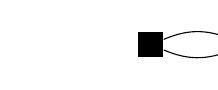
\begin{tikzpicture}[x=1.2cm]
 \node[rectangle,fill,minimum size=3.2mm,inner sep=0pt] (v0) at (0,0) {};
 \node[circle,draw,inner sep=1.2pt] (v1) at (1,0) {$0$};
 \draw (v0) to[bend left=22] (v1);
 \draw (v0) to[bend right=22] (v1);
 \draw (v1) edge[loop right] (v1);
\end{tikzpicture}
\end{center}
Its automorphism order is $2!\cdot2=4$. Write $t_1,t_2$ for the
connector variables and $s$ for the small loop variable, each in
$[0,\alpha]$. Its vertex polynomial is
$2\pi^2-t_1-t_2-2s$; the two flags of that loop both use $s$.
Integration in $s$ leaves $-\alpha(t_1+t_2)$, so its contribution
to $Q_{2,0}$ is
\begin{equation}\label{eq:s04:q-two-example}
 -\frac{\alpha}{4(8\pi^2)^2}\int_{[0,\alpha]^2}
 f(t_1)f(t_2)(t_1+t_2)\,\dd t_1\dd t_2
 =-1+\frac4{\pi^2}.
\end{equation}
The two connector moments were evaluated in the preceding subsection.
This is core $2.1$ of the appendix table. Its negative contribution
comes from the exact negative-psi polynomial.
\end{exm}

\begin{rmk}[Absolute normalization]
The $Q_{q,r}$ include the absolute WP corrections. In particular
the relative coefficient of Theorem~\ref{thm:s03:graph-expansion}
satisfies
\[
 e^{-S(1)}\gamma_1(1)=\frac98-c_1(0).
\]
At second order the conversion also includes $c_2(0)$ and the product
of the two first coefficients, as explained in
Subsection~\ref{subsec:a:02}.
\end{rmk}

\begin{rmk}[The absolute volume input]
The proof of Proposition~\ref{prp:a:c-two} uses the exact recursions
of \cite[Section~2]{MZ15} and \cite[Theorem~4.3]{HMT25}. Its
adjacent-genus comparison uses the actual fixed-marking expansion
through order three, so the unknown third volume coefficient cancels.
The result agrees with \cite[(6.10)]{EGGLS24}, derived there under
the resurgence assumption in Section~6.1 before (6.6). That conditional
prediction is a comparison after the reconstruction and is not a
proof input here.
\end{rmk}

\subsection{Proof of Theorem 1.1}
\label{subsec:s04:04}

It remains to combine the finite coefficient calculations with the
uniform estimates for the whole graph sum.

\begin{prfn}{Theorem~\ref{thm:lambda-one}}
Apply Proposition~\ref{prp:s03:graph-tail} with $M=3$ at $u=1$.
The absolute sum of graphs without a large vertex or with $q\geq3$
is $O(F_g g^{-3})$. There are only finitely many remaining core
types. First discard their legal loop counts $p>\log g$ by
Lemma~\ref{lmm:s03:loop-tail}. This tail is smaller than every fixed
inverse power after normalization, including when the large vertex's
genus is small.

For a remaining core of complexity $q\leq2$, apply
Proposition~\ref{prp:s03:core-expansion} with $K=2-q$.
All its intermediate volume types meet the uniform input thresholds
for $p\leq\log g$. There are constants $C>0$ and a fixed integer
$s\geq0$, depending on the core and expansion order, for which the
remainder after division by $V_{g,0}$ is bounded by
\[
 g^{-3}\frac{C^{p+1}(1+p)^s}{p!}.
\]
This bound sums to $O(g^{-3})$ over $p$.
The same factorial bound on the coefficient functions permits
extending each retained coefficient sum to all $p\geq0$, with a
further superpolynomially small tail. This is the extension used in
the signed moments above; no large-genus expansion has been applied
to an illegal or small-genus vertex.

Multiplication by~\eqref{eq:s03:fixed-n-volume} at $n=0$ through
order two converts the relative core expansions to the absolute
groups~\eqref{eq:s04:absolute-groups}. It preserves their summable
remainder bound and supplies the leading WP factor $1/\sqrt\pi$.
Consequently
\begin{align*}
 \frac{Z_g(1)}{F_g}=\frac{e^{S(1)}}{\sqrt\pi}
 \left[Q_{0,0}+\frac{Q_{0,1}+Q_{1,0}}g\right.\qquad\qquad\\
 \left.{}+\frac{Q_{0,2}+Q_{1,1}+Q_{2,0}}{g^2}
                  +O(g^{-3})\right].
\end{align*}
Propositions~\ref{prp:s04:first-correction}
and~\ref{prp:s04:second-correction} give the two coefficient sums.
Finally~\eqref{eq:s03:normalization-links} restores
$a_g/N_g=Z_g(1)/F_g$, and~\eqref{eq:s03:cin-identity} gives
$S(1)=\Cin(2\pi)$. Thus
\[
 a_g=\frac{e^{\Cin(2\pi)}}{\sqrt\pi}N_g
 \left[1+\frac{9}{8}g^{-1}
     +\left(\frac{257}{128}+\frac1{8\pi^2}\right)g^{-2}
     +O(g^{-3})\right],
\]
which is~\eqref{eq:111}.
\end{prfn}

\begin{samepage}
\begin{rmk}[Further coefficients]\label{rmk:s04:further-coefficients}
The same finite-core method gives further terms. For the normalized
quantity $\sqrt\pi\,e^{-\Cin(2\pi)}a_g/N_g$, the coefficients of
$g^{-3}$ and $g^{-4}$ are, respectively,
\begin{gather*}
 \frac{62909}{15360}+\frac{251}{192\pi^2}-\frac5{16\pi^4},\\
 \frac{291371}{32768}+\frac{129871}{15360\pi^2}
                    -\frac{277}{64\pi^4}+\frac{105}{64\pi^6}.
\end{gather*}
We omit the details of these calculations.
\end{rmk}
\end{samepage}


\section{Fixed degree Hodge insertions}
\label{sec:s05}

The identity $\lambda_3=\lambda_1^3/6+2\mathrm{ch}_3$ in
\eqref{eq:s02:lambda-two-three} isolates the first correction to a
fixed Hodge insertion. More generally, the Chern exponential expresses
every fixed product as powers of $\lambda_1$ multiplied by odd Chern
characters. We first show that a character of degree $a$ costs
$g^{1-a}$, with a bound on the complete decorated graph sum.
Consequently only one copy of $\mathrm{ch}_3$ can affect the terms
through $g^{-3}$.

The exact source formula below extends the boundary expansion to
labeled character insertions. Forgetting markings creates free
cotangent insertions, whose exponential factors must be retained.
The uniform estimates of Section~\ref{sec:s03} then justify the
finite-core calculation: a new free marking and a specified self-loop
supply the two contributions needed for $\mathrm{ch}_3$. The signed
loop functional of Section~\ref{sec:s04} evaluates their degree sums.
We finish by applying the Chern exponential to prove
Theorem~\ref{thm:fixed-insertions}. No second-order coefficient from
Theorem~\ref{thm:lambda-one} is needed.

\subsection{A filtration by odd Chern characters}
\label{subsec:s05:01}

We use the boundary exponential in
\cite[Lemma~3.10, (3.18)--(3.21)]{ABCDGLW23} for a general symmetric
node series. Its scalar specialization was proved in
Proposition~\ref{prp:s02:boundary-exponential}. We state the labeled
specialization and give its algebraic proof.

Fix an integer $r\geq1$ and odd integers $a_1,\ldots,a_r\geq3$,
and put $w=\sum_{i=1}^r a_i$. For an odd integer $a\geq3$ and formal variables $x,y$, define
the symmetric polynomial
\begin{equation}\label{eq:s05:node-polynomial}
 \mathcal P_a(x,y)=\sum_{c=0}^{a-1}(-1)^c x^c y^{a-1-c}.
\end{equation}
Let $\varepsilon_1,\ldots,\varepsilon_r$ be commuting formal
variables with $\varepsilon_i^2=0$. Coefficient extraction refers to
this square-free algebra. Set
\begin{equation}\label{eq:s05:source-kernel}
\begin{split}
 \mathcal E(x,y)&=\alpha+
       \sum_{i=1}^r\varepsilon_i\mathcal P_{a_i}(x,y),\\
 K_{\mathcal E}(x,y)&=
       \frac{1-e^{-(x+y)\mathcal E(x,y)}}{x+y}.
\end{split}
\end{equation}
The quotient is a formal series: its numerator is divisible by $x+y$.
All Chow series in the next identity are truncated by codimension.

\begin{lmm}[Labeled sources]\label{lmm:s05:labelled-sources}
For $g\geq2$,
\begin{align}
 &\int_{\MM_g}e^{12\alpha\lambda_1}
              \prod_{i=1}^r\mathrm{ch}_{a_i}\notag\\
 &=\left(\prod_{i=1}^r\frac{B_{a_i+1}}{(a_i+1)!}\right)
 [\varepsilon_1\cdots\varepsilon_r]
 \sum_{\Gamma\in\mathcal G_{g,0}}
 \frac1{|\operatorname{Aut}\Gamma|}\notag\\
 &\qquad\times\int_{\MM_\Gamma}
 \prod_{v\in V(\Gamma)}
  \exp\left(\alpha\kappa_1^{(v)}+
          \sum_{i=1}^r\varepsilon_i\kappa_{a_i}^{(v)}\right)
 \prod_{\substack{e\in E(\Gamma)\\e=\{f,f'\}}}
       K_{\mathcal E}(\psi_f,\psi_{f'}).
 \label{eq:s05:source-graphs}
\end{align}
\end{lmm}
\begin{prf}
On the unmarked space, \eqref{eq:s02:grr} writes each character as
$B_{a+1}/(a+1)!$ times
$\kappa_a+\tfrac12\xi_*\mathcal P_a(\psi_+,\psi_-)$.
Also $12\alpha\lambda_1=\alpha\kappa_1+\alpha\delta$.
The coefficient of the product of all the sources in the
exponential of these classes is their product, with no $r!$.

The normal line of a boundary branch has first Chern class
$-(x+y)$. Repeating that branch $k\geq1$ times in the exponential
therefore gives
\[
 \sum_{k\geq1}\frac{(-(x+y))^{k-1}\mathcal E(x,y)^k}{k!}
 =K_{\mathcal E}(x,y).
\]
Distinct nodes give the product of these factors, exactly as in the
proof of Proposition~\ref{prp:s02:boundary-exponential}. The
logarithmic dualizing line restricts to the logarithmic dualizing
line on each component, with the branches included among its
markings. Integrating its powers on the normalized universal curve
thus gives $\xi_\Gamma^*\kappa_a=\sum_v\kappa_a^{(v)}$.
The projection formula supplies the displayed vertex exponentials.

Finally, passing from labeled vertex and flag products to graph
isomorphism classes gives $1/|\operatorname{Aut}\Gamma|$.
The source labels remain distinct. Equivalently, grouping their
assignments into orbits gives the stabilizer of each decorated
graph; no permutation factor for the source labels is introduced.
All steps are self-intersection and pushforward operations in Chow,
so integration proves \eqref{eq:s05:source-graphs}.
\end{prf}

\begin{rmk}[Boundary normalization]
The cited lemma is stated in cohomology. Its normal-line proof,
spelled out above in the required specialization, is algebraic.
The source's boundary pushforward is the sum over one-edge graphs
with their automorphism factors. This equals our
$\tfrac12\xi_*$ on symmetric branch classes, already used in
\eqref{eq:s02:ordered-boundary}; no additional factor $1/2$ belongs
in \eqref{eq:s05:source-kernel}.
\end{rmk}

A source is assigned either to an edge or to a vertex. If a nonempty set
$J\subseteq[r]$ is assigned to one edge, its coefficient is
\begin{equation}\label{eq:s05:tagged-edge}
 [\textstyle\prod_{i\in J}\varepsilon_i]K_{\mathcal E}(x,y)
 =(-1)^{|J|-1}(x+y)^{|J|-1}e^{-\alpha(x+y)}
       \prod_{i\in J}\mathcal P_{a_i}(x,y).
\end{equation}
The polynomial multiplying the exponential has degree
$\sum_{i\in J}a_i-1$. An edge with no source retains
$K_\alpha(x,y)=\int_0^\alpha e^{-t(x+y)}\dd t$.

If a set $I\subseteq[r]$ is assigned to a vertex of type $(G,n)$,
use the partition inversion \eqref{eq:s02:partition-inversion}.
For each partition $\mathcal A$ of $I$, order its blocks as
$C_1,\ldots,C_m$, where $m=|\mathcal A|$; the expression is
independent of this order. For any polynomial, or
codimension-truncated series, $Q$ in the old cotangent classes,
\begin{align}
 &\int_{\MM_{G,n}}e^{\alpha\kappa_1}Q
                   \prod_{i\in I}\kappa_{a_i}\notag\\
 &=\sum_{\mathcal A\text{ a partition of }I}(-1)^{|I|-m}
   \int_{\MM_{G,n+m}}
    e^{\alpha\kappa_1-\alpha\sum_{k=1}^m\psi_{n+k}}
    Q
    \prod_{k=1}^m\psi_{n+k}^{\,1+\sum_{i\in C_k}a_i}.
 \label{eq:s05:free-markings}
\end{align}
For $I$ empty this means the original integral. Every new cotangent
power is at least four. Lemma~\ref{lmm:s02:rational-tail-degree}
therefore replaces the pullbacks of $Q$ by the intrinsic old classes
and replaces the pulled-back background by the exponential displayed
in \eqref{eq:s05:free-markings}. In particular the new factors
$e^{-\alpha\psi_{n+k}}$ survive. The inverse has the sign shown and
has no block factorials.

Each free new marking can return only one power of $g$ against the
loss $g^{-a}$ from degree conversion for a character of degree $a$.
We now justify this count for the complete graph sum, before using
it to discard any terms.

\begin{lmm}[Character filtration]\label{lmm:s05:character-filtration}
For the fixed indices above, as $g\to\infty$,
\begin{equation}\label{eq:s05:character-bound}
 \left\langle\prod_{i=1}^r\mathrm{ch}_{a_i}\right\rangle_g
       =O_{a_1,\ldots,a_r}(g^{r-w}).
\end{equation}
\end{lmm}
\begin{prf}
\emph{Uniform bounds on the original graphs.}
Estimate each term of \eqref{eq:s05:source-graphs} on its original
unmarked graph.
Let $s_v$ be the number of forgetting blocks at vertex $v$ and
$m=\sum_v s_v\leq r$. All cotangent insertions in
\eqref{eq:s05:tagged-edge} and \eqref{eq:s05:free-markings} are
fixed derivatives of vertex functions. Their total derivative order
is bounded in terms of the fixed $a_i$. Applying the multivariable
Cauchy formula on fixed discs to
Lemma~\ref{lmm:s03:vertex-bound} bounds each such derivative by the
same vertex majorant, with changed constants independent of the
stable type. Edge parameters lie in $[0,\alpha]$ or equal $\alpha$;
the discs lie in one fixed compact set. At a vertex with $s_v$ new
markings the factorial part changes by at most
\[
 \frac{\Gamma(k_v+s_v)}{\sqrt{k_v+s_v}}
 \leq(k_v+r)^{s_v}\frac{\Gamma(k_v)}{\sqrt{k_v}},
 \qquad k_v=2g_v-2+n_v\geq1.
\]
The other new factors are bounded constants depending on the indices.

In this counting paragraph put $H=2g-2$. Summing the assignments of
$m$ labeled blocks to vertices costs at most
\[
 \left(\sum_v(k_v+r)\right)^m
 \leq((r+1)H)^m,
\]
since $\sum_v k_v=H$ and $|V(\Gamma)|\leq H$.
There are only finitely many partitions of the fixed source labels.
Assigning the remaining labels to at most $r$ specified edges costs
at most $C_r(1+|E(\Gamma)|)^r$. This is absorbed into
$T^{|E(\Gamma)|}$ for a fixed $T>1$, rather than into another power
of $H$. Thus, even when absolute values are taken before the finite
source and partition sums, the complete graph term is bounded by
\begin{equation}\label{eq:s05:source-majorant}
 \frac{C(1+H)^rT^{|E(\Gamma)|}}{|\operatorname{Aut}\Gamma|}
 \prod_{v\in V(\Gamma)}
 \frac{C_1B^{n_v}(4\pi^2)^{k_v-1}\Gamma(k_v)}{\sqrt{k_v}}.
\end{equation}
All constants are independent of $g$ and $\Gamma$.

For every fixed integer $M\geq1$,
Corollary~\ref{crl:s03:marked-extension}\textup{(ii)}, applied to
these original graphs with no external legs and polynomial loss $r$,
now bounds the absolute contribution of graphs with no large vertex
or with $q\geq M$ by
\begin{equation}\label{eq:s05:source-tail}
 O_{a_1,\ldots,a_r,M}(F_g g^{r-M}).
\end{equation}

\emph{Fixed cores and all legal loop counts.}
Here $q$ and the core refer to the original unmarked graph, before
adding forgetting markings. Fix one core, a source assignment and
its partitions, and let $s$ be the number of their new markings at
the large vertex, so $0\leq s\leq r$. Its complexity after these
markings is $2g-2-q+s$, independently of the restored loop count
$p$. The all-type bound of Lemma~\ref{lmm:s03:vertex-bound} gives
the factorial ratio
$\Gamma(2g-2-q+s)/\Gamma(2g-2)=O(g^{s-q})$.
The small vertices have fixed types, and choices of specified
restored loops add only a fixed polynomial in $p$. Therefore, for
constants $C>0$ and an integer $A\geq0$ depending on these fixed
data, the absolute contribution with any legal $p$ is at most
\begin{equation}\label{eq:s05:decorated-core-bound}
 F_g g^{s-q}\frac{C^{p+1}(1+p)^A}{p!}.
\end{equation}
The all-type bound applies even when the large vertex's genus is
small. Summing over legal $p>\log g$ gives a remainder smaller
than any prescribed inverse power. Only after that truncation may
one use HMT's expansions on $p\leq\log g$, as in
Proposition~\ref{prp:s03:core-expansion}. In particular the bound
summed over all legal $p$ is $O(F_g g^{s-q})$.

Take $M=1$ in \eqref{eq:s05:source-tail}. The remaining finitely
many core assignments have $q=0$ and $s\leq r$, so their total is
$O(F_g g^r)$. Together with the tail this bounds the entire
integral in \eqref{eq:s05:source-graphs} by $O(F_g g^r)$.
Finally, for $3g-3\geq w$, degree conversion gives
\begin{equation}\label{eq:s05:character-normalization}
 \left\langle\prod_{i=1}^r\mathrm{ch}_{a_i}\right\rangle_g
 =(12\alpha)^w\frac{(3g-3-w)!}{(3g-3)!}
 \frac{\displaystyle\int_{\MM_g}e^{12\alpha\lambda_1}
                    \prod_{i=1}^r\mathrm{ch}_{a_i}}
      {Z_g(1)}.
\end{equation}
The factorial prefactor is $O(g^{-w})$.
Theorem~\ref{thm:s03:graph-expansion} gives
$Z_g(1)\sim e^{S(1)}V_{g,0}$.
Since $V_{g,0}\asymp F_g$, this proves
\eqref{eq:s05:character-bound}.
\end{prf}

The Chern exponential now reduces the theorem to one character.

\begin{crl}[Algebraic reduction]\label{crl:s05:algebraic-reduction}
For the fixed product in Theorem~\ref{thm:fixed-insertions},
\begin{equation}\label{eq:s05:algebraic-reduction}
 F(j)\langle P(\lambda)\rangle_g
 =1+2G(j)\langle\mathrm{ch}_3\rangle_g+O(g^{-4}).
\end{equation}
\end{crl}
\begin{prf}
For a homogeneous Hodge polynomial $Q$ and an integer $c\geq0$
with $\deg Q+c\leq3g-3$, the definition of the normalized bracket
gives the exact identity
$\langle\lambda_1^c Q\rangle_g=\langle Q\rangle_g$.
In \eqref{eq:s02:chern-exponential}, the term with no character of
degree at least three contributes $\lambda_1^{j_k}/j_k!$ to
$\lambda_{j_k}$. The term with one $\mathrm{ch}_3$ contributes
$2\mathrm{ch}_3\lambda_1^{j_k-3}/(j_k-3)!$ when $j_k\geq3$.
Multiplying the fixed factors and then $F(j)$ gives the coefficient
$2\sum_{k=1}^{\ell}j_k(j_k-1)(j_k-2)=2G(j)$.

Every other nonconstant term has either one odd character of degree
at least five, or at least two characters of degrees at least three.
Lemma~\ref{lmm:s05:character-filtration} makes each such normalized
term $O(g^{-4})$. There are only finitely many terms, since the
$j_k$ are fixed. Indices below three simply supply no
$\mathrm{ch}_3$ term, completing the proof.
\end{prf}

\subsection{The two leading coefficients of a single character}
\label{subsec:s05:02}

For one source of degree three, let $T_g^{\rm free}$ and
$T_g^{\rm edge}$ denote the graph sums in
\eqref{eq:s05:source-graphs} with that source assigned, respectively,
to a vertex or to an edge, omitting the Bernoulli prefactor. Thus
\begin{equation}\label{eq:s05:single-source}
 \int_{\MM_g}e^{12\alpha\lambda_1}\mathrm{ch}_3
       =-\frac1{720}(T_g^{\rm free}+T_g^{\rm edge}).
\end{equation}
A free marking gives the leading term. At the next order, terms
from free markings on the $q=1$ cores cancel against the corresponding
denominator terms.
A specified self-loop on the $q=0$ core remains. We calculate both
parts before conversion to the normalized Hodge bracket.

\begin{lmm}[One source]\label{lmm:s05:single-source}
As $g\to\infty$,
\begin{align}
 \frac{T_g^{\rm free}}{8\pi^2gZ_g(1)}
 &=f^{(4)}(\alpha)-\frac{5f^{(4)}(\alpha)}{4g}\notag\\
 &\quad-\frac{9f^{(4)}(\alpha)
          +\tfrac{15}{2}\alpha f^{(5)}(\alpha)
          +\alpha^2 f^{(6)}(\alpha)}{\pi^2g}
          +O(g^{-2}),
 \label{eq:s05:free-ratio}\\
 \frac{T_g^{\rm edge}}{Z_g(1)}
 &=-\frac12 f'(\alpha)^2+O(g^{-1}).
 \label{eq:s05:edge-ratio}
\end{align}
\end{lmm}
\begin{prf}
\emph{Truncation before expansion.}
Use \eqref{eq:s05:source-tail} with $r=1$ and $M=2$.
All graphs with no large vertex or with $q\geq2$ contribute
$O(F_g g^{-1})$ to either source sum. On the remaining cores,
\eqref{eq:s05:decorated-core-bound} discards every legal
$p>\log g$ before a large-genus expansion is used. For
$p\leq\log g$ the large genus is $g-O(\log g)$ and its valence is
$O(\log g)$. The HMT thresholds and summable remainder argument in
Proposition~\ref{prp:s03:core-expansion} therefore apply, also after
the fixed derivatives just used in the majorant proof.
Lemma~\ref{lmm:s03:degree-moments} sums their polynomial degree
errors. In this way a relative error $O(g^{-2})$ in a free-marking
term of size $F_g g$ is $O(F_g g^{-1})$ after summation. Only leading
terms are needed for the specified-edge part of size $F_g$.

\emph{The common $q=1$ terms.}
A free marking on a small vertex of a $q=1$ core has $s=0$ in
\eqref{eq:s05:decorated-core-bound}, so it is already
$O(F_g g^{-1})$.

A free marking on the large vertex instead
multiplies the leading contribution of that same core by
$8\pi^2g f^{(4)}(\alpha)$. Indeed its leading volume ratio is
$8\pi^2g$, and its differentiated leg factor is
$f^{(4)}(\alpha)$. The core, its small-vertex integrals, its
loop weights and its automorphism factor are unchanged.
This is an additive identity of leading terms for each core and
loop count, without division by a leg factor.

Consequently all $q=1$ contributions to $T_g^{\rm free}/(8\pi^2g)$ equal
$f^{(4)}(\alpha)$ times their denominator contributions at order
$g^{-1}$ and cancel on dividing by $Z_g(1)$. The unmodified
first corrections on the $q=0$ graph cancel in the same way.
We are left with the increment caused by the new marking on that
graph. A specified edge on a $q=1$ core is
$O(F_g g^{-1})$ and needs no coefficient calculation.

\emph{The free-marking increment.}
Write $G=g-p$ and $n=2p$ on the one-vertex graph, and let
$\mathbf d$ be its old degree tuple, with total $D$ and zero count
$m_0$. The first volume coefficient \eqref{eq:s03:c-one} gives
\begin{equation}\label{eq:s05:one-mark-volume}
 \frac{V_{G,n+1}}{8\pi^2G V_{G,n}}
 =1+\frac{n/2-5/4+(2-n)/\pi^2}{G}+O(G^{-2}).
\end{equation}
For fixed $n$ this follows directly by dividing
\eqref{eq:s03:fixed-n-volume}; on the retained growing valences its
coefficients and polynomial remainders have the uniform meaning
established in Section~\ref{sec:s03}. Including $G/g=1-p/g$, the
extra volume factor at order $g^{-1}$ is
$-5/4+(2-2p)/\pi^2$.

The new marking in \eqref{eq:s05:free-markings} has a factor
$\psi_{n+1}^4e^{-\alpha\psi_{n+1}}$. Its descendant degree
$d\geq4$ is therefore always positive, and $m_0$ does not change.
The first profile \eqref{eq:a:first-profile} gives the exact
polynomial difference
\begin{align}
 &e_{n+1,1}(\mathbf d,d)-e_{n,1}(\mathbf d)\notag\\
 &\quad=-\frac{4Dd+2d^2+2D+(2n-3)d-n+2}{\pi^2}.
 \label{eq:s05:profile-increment}
\end{align}
This also holds for the empty old tuple. By
\eqref{eq:a:profile-genus-conversion}, half this difference is the
increment of the coefficient of $G^{-1}$; its source expansion is
in $(2G-2+n)^{-1}$, rather than $G^{-1}$.

For a complex degree-generating variable $z$, put
$\varphi(z)=z^4f^{(4)}(\alpha z)$. Its coefficient of $z^d$
is the weight of the new degree $d$, since differentiating a term
$t^d$ four times leaves degree-counting factor $z^d$.
All these series, also with any fixed degree moment, converge
absolutely. The joint generator of Lemma~\ref{lmm:s04:loop-moments}
gives $\mathcal L[p]=S(1)$, while
\eqref{eq:s04:representative-moments} gives
$\mathcal L[D]=-S(1)$. Substituting $n=2p$ into
\eqref{eq:s05:profile-increment} yields, for each integer $d\geq4$,
\begin{equation}\label{eq:s05:averaged-increment}
 \frac12\mathcal L\left[
   e_{2p+1,1}(\mathbf d,d)-e_{2p,1}(\mathbf d)\right]
 =\frac{2S(1)-d^2+3d/2-1}{\pi^2}.
\end{equation}
The volume increment contributes
$[-5/4+(2-2S(1))/\pi^2]\varphi(1)$.
Adding \eqref{eq:s05:averaged-increment} with weights
$[z^d]\varphi(z)$ cancels $S(1)$. The first correction in the
free ratio is consequently
\begin{equation}\label{eq:s05:free-moment}
 -\frac54\varphi(1)+\frac1{\pi^2}
 \left[\varphi(1)+\left.
  \left(\frac32z\partial_z-(z\partial_z)^2\right)
                  \varphi(z)\right|_{z=1}\right].
\end{equation}
Here
\begin{align*}
 \varphi(1)&=f^{(4)}(\alpha),\\
 (z\partial_z)\varphi(z)|_{z=1}
       &=4f^{(4)}(\alpha)+\alpha f^{(5)}(\alpha),\\
 (z\partial_z)^2\varphi(z)|_{z=1}
       &=16f^{(4)}(\alpha)+9\alpha f^{(5)}(\alpha)
                                     +\alpha^2f^{(6)}(\alpha).
\end{align*}
Substitution proves \eqref{eq:s05:free-ratio}.

\emph{The specified self-loop.}
By \eqref{eq:s05:tagged-edge}, the edge coefficient is
\[
 \mathcal P_3(x,y)e^{-\alpha(x+y)},\qquad
 \mathcal P_3(x,y)=x^2-xy+y^2.
\]
There is no remaining factor $1/(x+y)$ and no integration in the
specified edge parameter.
For $p\geq1$ loops, specifying one of them changes the symmetry
factor by
\begin{equation}\label{eq:s05:specified-loop-weight}
 \frac{p}{2^pp!}=\frac1{2\,2^{p-1}(p-1)!}.
\end{equation}
The other loops sum to $e^{S(1)}$. The specified loop therefore
contributes the factor
\[
 \frac12\left(2f(\alpha)f''(\alpha)-f'(\alpha)^2\right)
       =-\frac12f'(\alpha)^2,
\]
where $f(\alpha)=0$ was used. Its branch-exchange factor $1/2$
has been counted exactly once in
\eqref{eq:s05:specified-loop-weight}. Dividing by the leading
$e^{S(1)}V_{g,0}$ cancels the other loops and the volume factor.
The already controlled remainder is $O(g^{-1})$, proving
\eqref{eq:s05:edge-ratio}.
\end{prf}

Only finitely many derivatives are now needed. For each integer
$k\geq0$ define
\begin{equation}\label{eq:s05:endpoint-derivatives}
 X_k=(8\pi^2)^k f^{(k)}(\alpha).
\end{equation}

\begin{lmm}[Endpoint derivatives]\label{lmm:s05:endpoint-derivatives}
These values satisfy
\begin{equation}\label{eq:s05:derivative-recurrence}
 X_0=0,\quad X_1=-2,\qquad
 X_{k+2}=-(4k+6)X_{k+1}-4\pi^2X_k\quad(k\geq0).
\end{equation}
The required finite list is
\begin{center}
\begin{tabular}{c|l}
$k$ & $X_k$ \\\hline
$0$ & $0$ \\
$1$ & $-2$ \\
$2$ & $12$ \\
$3$ & $8(\pi^2-15)$ \\
$4$ & $1680-160\pi^2$ \\
$5$ & $-32(\pi^4-105\pi^2+945)$ \\
$6$ & $1344(\pi^4-60\pi^2+495)$
\end{tabular}
\end{center}
\end{lmm}
\begin{prf}
The series \eqref{eq:s03:loop-functions} gives
$8tf''(t)+12f'(t)+f(t)=0$. Differentiating $k$ times gives
$8tf^{(k+2)}+(8k+12)f^{(k+1)}+f^{(k)}=0$.
At $t=\alpha=2\pi^2$ this is precisely the recurrence after the
rescaling \eqref{eq:s05:endpoint-derivatives}.
The sine formula gives $f(\alpha)=0$ and
$f'(\alpha)=-1/(4\pi^2)$, hence the two initial values.
Successive substitution gives the table.
\end{prf}

The next calculation includes the factorial conversion in the free
term. Both contributions then have the Hodge bracket normalization.

\begin{prp}[The third character]\label{prp:s05:third-character}
As $g\to\infty$,
\begin{equation}\label{eq:s05:third-character}
 \langle\mathrm{ch}_3\rangle_g
 =\frac{2\pi^2-21}{9g^2}
       +\frac{2(\pi^2-10)}{3g^3}+O(g^{-4}).
\end{equation}
\end{prp}
\begin{prf}
The factor in \eqref{eq:s05:character-normalization} is
\begin{equation}\label{eq:s05:factorial-three}
 (12\alpha)^3\frac{(3g-6)!}{(3g-3)!}
 =\frac{(8\pi^2)^3}{g^3}
             \left(1+\frac4g+O(g^{-2})\right).
\end{equation}
Combining \eqref{eq:s05:single-source} and
\eqref{eq:s05:free-ratio}, the leading coefficient of $g^{-2}$
is $-X_4/720=(2\pi^2-21)/9$.

The free-marking coefficient at order $g^{-3}$, including the
$4/g$ in \eqref{eq:s05:factorial-three}, is
\begin{equation}\label{eq:s05:free-coefficient}
 -\frac1{720}\left[
 \frac{11}{4}X_4-
 \frac{9X_4+15X_5/8+X_6/16}{\pi^2}\right]
 =\frac{29\pi^2}{45}-\frac{20}{3}.
\end{equation}

For the specified loop, \eqref{eq:s05:edge-ratio} gives
\begin{equation}\label{eq:s05:loop-coefficient}
 -\frac{(8\pi^2)^3}{720}
           \left(-\frac12f'(\alpha)^2\right)=\frac{\pi^2}{45}.
\end{equation}

Adding the last two values gives $2(\pi^2-10)/3$.
The $O(g^{-1})$ error before degree conversion, including all graph,
loop and degree tails in Lemma~\ref{lmm:s05:single-source}, becomes
$O(g^{-4})$. The unused second relative term of
\eqref{eq:s05:factorial-three} has the same order after multiplication
by the leading free term. This proves the proposition.
\end{prf}

\subsection{Proof of Theorem 1.2 and examples}
\label{subsec:s05:03}

Substituting the single-character expansion into the algebraic
reduction proves the theorem.

\begin{prfn}{Theorem~\ref{thm:fixed-insertions}}
The indices $j_1,\ldots,j_\ell$ are fixed, so all the classes and
powers in Corollary~\ref{crl:s05:algebraic-reduction} are defined
for sufficiently large $g$. By that corollary and
Proposition~\ref{prp:s05:third-character},
\[
 \langle P(\lambda)\rangle_g
 =\frac1{F(j)}\left[
 1+\frac{4\pi^2-42}{9g^2}G(j)
  +\frac{4\pi^2-40}{3g^3}G(j)+O(g^{-4})\right].
\]
The error constant may depend on the fixed list of indices.
This is \eqref{eq:P111}.
\end{prfn}

\begin{exm}[Indices at most two]
If every $j_k$ is one or two, then
\eqref{eq:s02:lambda-two-three} gives
\[
 \left\langle\prod_{k=1}^{\ell}\lambda_{j_k}\right\rangle_g
 =2^{-\#\{k:j_k=2\}}=\frac1{F(j)}
\]
exactly whenever the total degree is at most $3g-3$.
In this case $G(j)=0$, in agreement with the theorem.
\end{exm}

\begin{exm}[A single third Chern class]
The exact relation
$6\langle\lambda_3\rangle_g=1+12\langle\mathrm{ch}_3\rangle_g$
gives
\[
 \langle\lambda_3\rangle_g
 =\frac16+\frac{4\pi^2-42}{9g^2}
          +\frac{4(\pi^2-10)}{3g^3}+O(g^{-4}).
\]
These are precisely $F(j)=6$ and $G(j)=6$ in the theorem.
\end{exm}

\begin{exm}[Two fixed classes]
For $\lambda_{j_1}\lambda_{j_2}$ the correction is proportional to
$j_1(j_1-1)(j_1-2)+j_2(j_2-1)(j_2-2)$.
Selecting one $\mathrm{ch}_3$ from each factor instead gives
$\mathrm{ch}_3^2$, whose bracket is $O(g^{-4})$ by
Lemma~\ref{lmm:s05:character-filtration}. Thus through order
$g^{-3}$ only the sum of the two individual coefficients appears.
\end{exm}


\section{The top Hodge class and Bessel asymptotics}
\label{sec:s06}

This section proves Theorem~\ref{thm:top-hodge}. The top-class
restriction in Corollary~\ref{crl:s02:defect-allocation} removes
every graph with a cycle and factors $\lambda_g$ over the remaining
trees. Together with degree conversion from
Section~\ref{sec:s02}, the boundary exponential
\eqref{eq:s02:boundary-exponential} turns the integral defining $b_g$
into a sum of top-Hodge vertex integrals.

We first use the $\lambda_g$ theorem to reduce each vertex to a
one-variable coefficient. A strict modulus estimate on a Bessel
circle gives a bound uniform in all stable vertex types. This bound
controls the complete tree tail, leaving only the tree with no
edges and an elliptic leaf at the required precision. A two-term
saddle calculation and the leaf integral then determine the three
terms in the scalar $b$.

The exact genus-zero reduction, classical Bessel inverse and
critical-point data are also retained for the later fixed-defect
analysis.

\subsection{Top Hodge intersections and exact vertices}
\label{subsec:s06:01}

We use Faber--Pandharipande's multipoint theorem
\cite[Theorem~1]{FP03}, together with their earlier one-point
calculation \cite[Theorem~2, (6)]{FP00}. Set $\beta_0=1$ by
convention and, for an integer $G\geq1$, define
\begin{equation}\label{eq:s06:beta-definition}
 \beta_G=\int_{\MM_{G,1}}\lambda_G\psi_1^{2G-2}.
\end{equation}
We write $\beta_G$ for the coefficients denoted by $b_G$ in
\cite[(3), (6)]{FP00}.
In particular $\beta_0$ is not an integral on a genus-zero one-point
space.

\begin{thm}[Top Hodge intersections]\label{thm:s06:lambda-g}
For integers $G\geq1$, $N\geq1$ and nonnegative integers
$d_1,\ldots,d_N$ with $\sum_i d_i=2G-3+N$,
\begin{equation}\label{eq:s06:lambda-g}
 \int_{\MM_{G,N}}\lambda_G\prod_{i=1}^N\psi_i^{d_i}
 =\beta_G\frac{(2G-3+N)!}{\prod_{i=1}^N d_i!}.
\end{equation}
The same formula holds for $G=0$, $N\geq3$ with $\beta_0=1$.
For a formal variable $z$,
\begin{equation}\label{eq:s06:beta-series}
 \sum_{G\geq0}\beta_Gz^{2G}=\frac{z/2}{\sin(z/2)}.
\end{equation}
As $G\to\infty$,
\begin{equation}\label{eq:s06:beta-asymptotics}
 \beta_G=2(2\pi)^{-2G}(1+O(4^{-G})),\qquad
 \frac{\beta_{G-1}}{\beta_G}=(2\pi)^2(1+O(4^{-G})).
\end{equation}
There are absolute constants $c,C>0$ such that
$c(2\pi)^{-2G}\leq\beta_G\leq C(2\pi)^{-2G}$ for every $G\geq0$.
\end{thm}
\begin{prf}
The positive-genus formula is \cite[Theorem~1]{FP03}; the
stable genus-zero formula is its equation~(1). The generating
series is \cite[Theorem~2, (6)]{FP00}, whose genus-zero value is
one. For real $s>1$, write
$\zeta(s)=\sum_{k\geq1}k^{-s}$ for the Riemann zeta function.
The Bernoulli evaluation in \cite[\S 4.2, Lemma~1]{FP00}
and \cite[(25.6.2)]{DLMF} give, for $G\geq1$,
\[
 \beta_G=(1-2^{1-2G})\frac{|B_{2G}|}{(2G)!}
       =2(1-2^{1-2G})\zeta(2G)(2\pi)^{-2G}.
\]
The Dirichlet series \cite[(25.2.1)]{DLMF} implies
$\zeta(2G)=1+O(4^{-G})$ as $G\to\infty$.
This proves both asymptotics and the uniform comparison, extending
the constants to the finitely many small genera and $G=0$.
\end{prf}

For $x\in\mathbb C$, define the entire function
\begin{equation}\label{eq:s06:phi}
 \Phi(x)=\sum_{a\geq0}\frac{(-1)^a x^a}{a!(a+1)!}
        =\frac{J_1(2\sqrt x)}{\sqrt x}.
\end{equation}
The quotient and every subsequent square-root expression in Bessel
functions mean their entire power series.

For a stable pair $(G,n)$, let $\mathbf s=(s_1,\ldots,s_n)$
be a complex vector and set
\begin{equation}\label{eq:s06:vertex-definition}
 W^{\rm top}_{G,n}(\mathbf s)
  =\int_{\MM_{G,n}}\lambda_G
                   e^{\kappa_1-\sum_{i=1}^n s_i\psi_i}.
\end{equation}
The superscript distinguishes this vertex integral from other
intersection generating functions. The local coefficient order
$m=2G-3+n$ is nonnegative for every stable type.

The whole exponential specialization
\eqref{eq:s02:kappa-exponential} is especially useful here. It
replaces the background by new cotangent insertions, after which
\eqref{eq:s06:lambda-g} determines every coefficient.

\begin{prp}[Exact vertices]\label{prp:s06:exact-vertex}
For every stable pair $(G,n)$, with $m=2G-3+n$,
\begin{equation}\label{eq:s06:exact-vertex}
 W^{\rm top}_{G,n}(\mathbf s)
 =\beta_G m![x^m]\Phi(x)^{-m-1}
                       \prod_{i=1}^n J_0(2\sqrt{s_i x}).
\end{equation}
\end{prp}
\begin{prf}
Apply \eqref{eq:s02:kappa-exponential} with scalar parameter one.
A term with $k\geq0$ forgotten points has coefficient $1/k!$ and
new-point factor $\psi(1-e^{-\psi})$ at each point.
The Hodge insertion pulls back unchanged. The new powers have
minimum degree two, so Lemma~\ref{lmm:s02:rational-tail-degree}
replaces the old cotangent pullbacks by their intrinsic classes.
This is the inversion of the entire kappa background; there is no
further background exponential to pull back.

The multinomial formula contributes $\beta_G(m+k)!$ and a
factorial denominator for each descendant degree. Thus the old
marking $i$ contributes
\[
 \sum_{a\geq0}\frac{(-s_i x)^a}{(a!)^2}
       =J_0(2\sqrt{s_i x}),
\]
whereas a new marking contributes
\[
 \sum_{a\geq1}\frac{(-1)^{a-1}x^{a+1}}{a!(a+1)!}
       =x(1-\Phi(x)).
\]
After removing $x^k$ from the coefficient extraction, the vertex
integral is therefore
\[
 \beta_G[x^m]\prod_{i=1}^nJ_0(2\sqrt{s_i x})
       \sum_{k\geq0}\frac{(m+k)!}{k!}(1-\Phi(x))^k.
\]
This sum is coefficientwise finite because $1-\Phi(x)$ has zero
constant term. The binomial series makes it
$m!\Phi(x)^{-m-1}$, proving the formula.

For an unmarked vertex $G\geq2$, one has $m\geq1$. Its $k=0$
term vanishes by degree, and every nonzero term has at least one
marking, as required by the positive-genus multipoint theorem.
For $G=0$ the original stability already gives $n\geq3$.
These observations cover the ranges excluded from a literal
application of \eqref{eq:s06:lambda-g} with $N=0$.
\end{prf}

\begin{crl}[Numerical genus-zero reduction]\label{crl:s06:genus-zero}
For every stable type,
\begin{equation}\label{eq:s06:genus-zero}
 W^{\rm top}_{G,n}(\mathbf s)
 =\beta_G W^{\rm top}_{0,2G+n}(\mathbf s,0,\ldots,0).
\end{equation}
\end{crl}
\begin{prf}
The type on the right is stable since $2G+n=m+3\geq3$.
It has the same coefficient order $m$, and its additional $2G$
old-marking factors are $J_0(0)=1$ in
\eqref{eq:s06:exact-vertex}. Its one-point convention is $\beta_0=1$.
\end{prf}

\begin{rmk}[Classical inverse]
This is an equality of numerical generating functions on different
moduli spaces. The inverse of $x\mapsto x\Phi(x)$ is the classical
genus-zero kappa series of \cite[(0.8)]{KMZ96v1}, with its earlier
Zograf attribution. For a formal variable $t$ and an integer $N\geq3$,
Lagrange inversion and \eqref{eq:s06:exact-vertex} give its
$t^{N-2}$ coefficient as
\[
 \frac{W^{\rm top}_{0,N}(\mathbf0)}{(N-2)!}
 =\frac{\displaystyle\int_{\MM_{0,N}}\kappa_1^{N-3}}
        {(N-2)!(N-3)!}.
\]
This makes the conversion from raw kappa powers to exponential
integrals explicit. The inverse and critical behavior are also
analyzed in \cite[\S 6, Proof~6.3]{MaZ00}. The uniform vertex
and complete tree estimates needed here will be proved directly.
\end{rmk}

\subsection{The Bessel critical point and uniform bounds}
\label{subsec:s06:02}

Using the zero fixed in the Introduction, define
\begin{equation}\label{eq:s06:critical-data}
 x_* =\frac{z_{0,1}^2}{4},\qquad
 w(x)=x\Phi(x),\qquad
 R=w(x_*)=\frac{z_{0,1}J_1(z_{0,1})}{2}=\frac{\rho}{12}.
\end{equation}
The strict circle estimate below makes this positive point the
unique dominant point of the Cauchy integral. It also supplies a
bound that is uniform when both the genus and the valence vary.

\begin{lmm}[Critical circle]\label{lmm:s06:critical-circle}
The function $\Phi$ has no zero on $|x|\leq x_*$, and
\begin{equation}\label{eq:s06:critical-derivatives}
 w'(x)=J_0(2\sqrt x),\quad w'(x_*)=0,\quad
 w''(x_*)=-\frac{2J_1(z_{0,1})}{z_{0,1}}<0.
\end{equation}
There is a constant $a>0$ such that, for $-\pi\leq\theta\leq\pi$,
\begin{equation}\label{eq:s06:circle-bound}
 |\Phi(x_*e^{i\theta})|
       \geq\Phi(x_*)e^{a\theta^2}.
\end{equation}
In particular $R>0$.
\end{lmm}
\begin{prf}
For an integer $k\geq1$, let $z_{1,k}$ be the $k$th positive zero
of $J_1$. The product \cite[(10.21.15)]{DLMF} gives
\begin{equation}\label{eq:s06:phi-product}
 \Phi(x)=\prod_{k\geq1}\left(1-\frac{4x}{z_{1,k}^2}\right).
\end{equation}
Interlacing \cite[(10.21.2)]{DLMF} gives
$z_{0,1}<z_{1,1}$. Thus all factors are positive at $x_*$ and all
zeros of $\Phi$ lie outside its closed disk.
The derivative identities \cite[(10.6.6), (10.6.3)]{DLMF} give
\eqref{eq:s06:critical-derivatives}. Also $J_1$ is positive between
zero and $z_{1,1}$, so $J_1(z_{0,1})>0$ and $R>0$.

For $0<u<1$ one has
\[
 |1-ue^{i\theta}|^2=(1-u)^2+2u(1-\cos\theta).
\]
Consequently each factor of \eqref{eq:s06:phi-product} has modulus
at least its value at $x_*$. For the first factor, the logarithm
of the ratio divided by $\theta^2$ extends to a strictly positive
continuous function at zero and is positive elsewhere on
$[-\pi,\pi]$. Its positive minimum gives $a$ in
\eqref{eq:s06:circle-bound}; the other factors only improve the
bound. The convergent product permits passage from finite products
to $\Phi$.
\end{prf}

\begin{rmk}[Critical-value convention]
The critical value denoted $x_0$ in
\cite[\S 6, (17) and Proof~6.3]{MaZ00} is our $R$.
Our positive critical argument $x_*$ and its derivative properties
are fixed by \eqref{eq:s06:critical-data} and proved above.
\end{rmk}

\begin{lmm}[All stable vertex types]\label{lmm:s06:vertex-bound}
There is a constant $C>0$, independent of the stable type $(G,n)$,
such that for $s_i\in[0,1]$ and $m=2G-3+n$,
\begin{equation}\label{eq:s06:vertex-bound}
 |W^{\rm top}_{G,n}(\mathbf s)|
 \leq C^{n+1}\beta_G\frac{m!R^{-m}}{\sqrt{m+1}}.
\end{equation}
\end{lmm}
\begin{prf}
On $|x|=x_*$, the entire series for $J_0$ gives the bound
\[
 |J_0(2\sqrt{s x})|
 \leq\sum_{k\geq0}\frac{x_*^k}{(k!)^2}
 \qquad(0\leq s\leq1).
\]
Its right side is a fixed finite constant. Cauchy's formula and
\eqref{eq:s06:circle-bound} bound the coefficient in
\eqref{eq:s06:exact-vertex} by
\[
 C^n x_*^{-m}\Phi(x_*)^{-m-1}
 \frac1{2\pi}\int_{-\pi}^{\pi}e^{-a(m+1)\theta^2}\dd\theta
 \leq\frac{C^{n+1}R^{-m}}{\sqrt{m+1}}.
\]
Multiplication by $\beta_Gm!$ proves the assertion, also for $m=0$.
The constants depend only on the fixed circle, not on $G$ or $n$.
\end{prf}

\subsection{Stable trees and their tails}
\label{subsec:s06:03}

For a vertex $v$ of a tree, put $m_v=2g_v-3+n_v$. Let
$\mathbf s_v$ be its tuple of flag parameters: both flags belonging
to an edge $e$ use the same $s_e\in[0,1]$.
For the comparisons in this and the next subsection define the
positive scale
\begin{equation}\label{eq:s06:tree-scale}
 \mathcal T_g=\beta_g\frac{g_2!R^{-g_2}}{\sqrt{g_2+1}}.
\end{equation}
We first keep the exact automorphism factors. Only after bounding
every vertex will we replace unrooted trees by plane rooted trees
in a positive majorant. This controls the entire genus and valence
sum at each edge count.

\begin{prp}[The complete tree sum]\label{prp:s06:tree-tail}
For $g\geq2$,
\begin{equation}\label{eq:s06:tree-expansion}
 \frac{12^{g_2}b_g}{g_2!}
 =\sum_{\substack{\Gamma\in\mathcal G_{g,0}\\\Gamma\text{ a tree}}}
  \frac1{|\operatorname{Aut}\Gamma|}
  \int_{[0,1]^{E(\Gamma)}}
       \prod_{v\in V(\Gamma)}W^{\rm top}_{g_v,n_v}(\mathbf s_v)
       \prod_{e\in E(\Gamma)}\dd s_e.
\end{equation}
Every contributing tree has $E\leq g_2$ edges. There is a constant
$C>0$, independent of $g$ and $E$, such that the absolute sum of
its $E$-edge integrals is at most
\begin{equation}\label{eq:s06:edge-mass}
 \mathcal T_g C^{E+1}
 \sqrt{\frac{g_2+1}{g_2-E+1}}\,
                  \frac{(g_2-E)!}{g_2!}
 \qquad(0\leq E\leq g_2).
\end{equation}
Hence, for every fixed integer $K\geq1$, the sum over all trees
with at least $K$ edges is $O_K(\mathcal T_g g_2^{-K})$ in
absolute value.
\end{prp}
\begin{prf}
\emph{The finite-genus identity.}
The boundary exponential with both scalar coefficients one gives
edge kernel $\int_0^1e^{-s(\psi_f+\psi_{f'})}\dd s$.
By Corollary~\ref{crl:s02:defect-allocation}, the pullback of
$\lambda_g$ vanishes on every graph with a cycle and is the product
of the vertex top classes on a tree. Logarithmic kappa additivity
\eqref{eq:s02:tautological-gluing} now gives the right side of
\eqref{eq:s06:tree-expansion}, with the original graph
$1/|\operatorname{Aut}\Gamma|$.
On the left, $\kappa_1+\delta=12\lambda_1$ and degree conversion
gives $\int\lambda_ge^{12\lambda_1}=12^{g_2}b_g/g_2!$.
For a tree, the genus condition and flag count imply
\begin{equation}\label{eq:s06:tree-degree}
 \sum_v m_v=\sum_v(2g_v-3+n_v)=g_2-E.
\end{equation}
All $m_v$ are nonnegative, proving $E\leq g_2$.

\emph{A majorant for every tree and genus assignment.}
The comparison for $\beta_G$ in Theorem~\ref{thm:s06:lambda-g}
uses $\sum_v g_v=g$ to give
$\prod_v\beta_{g_v}\leq C^{E+1}\beta_g$, including rational and
elliptic vertices. Apply Lemma~\ref{lmm:s06:vertex-bound} to
every factor. Since $\sum_v n_v=2E$ and there are $E+1$ vertices,
all its exponential constants are bounded by $C^{E+1}$ after
increasing $C$. The edge domains have measure one. After removing
$\beta_gR^{-g_2}$, the remaining majorant is thus a constant to
power $E+1$ times
$\prod_v m_v!/\sqrt{m_v+1}$.

Every unrooted genus-labeled tree has a plane rooted realization,
and its original weight is at most one. A plane rooted tree with
$E$ edges is encoded by a walk of $2E$ up/down steps, so there are
at most $4^E$ shapes. For a fixed shape and the $m_v$, the genus
labels are determined by $2g_v=m_v+3-n_v$. The beta factors have
already been bounded uniformly; dropping parity and stability restrictions
therefore only enlarges the positive sum over nonnegative $m_v$.
This introduces no factorial in the vertex count.

For every integer $M\geq0$,
\begin{equation}\label{eq:s06:factorial-convolution}
 \sum_{k=0}^M k!(M-k)!\leq3M!.
\end{equation}
Indeed the two endpoint terms give $2M!$ when $M\geq1$, while
$\binom{M}{k}\geq M$ for $1\leq k\leq M-1$; the case $M=0$
is immediate.

Iterating the convolution for $E+1$ vertices gives
$3^EM!$ for total $M=\sum_v m_v$. Also
$\prod_v(m_v+1)\geq M+1$. With $M=g_2-E$, these estimates and
the shape count prove \eqref{eq:s06:edge-mass}.

\emph{Summing every edge count.}
For $0\leq E\leq g_2$, direct multiplication gives
\[
 (E+1)(g_2-E+1)-(g_2+1)=E(g_2-E)\geq0.
\]
The square root in \eqref{eq:s06:edge-mass} is therefore at most
$\sqrt{E+1}$. Moreover
\[
 \frac{(g_2-E)!}{g_2!}\leq\left(\frac e{g_2}\right)^E.
\]
For example, integrate $\log t$ from $g_2-E$ to $g_2$ to bound
the logarithm of the falling factorial below by
$E(\log g_2-1)$. For sufficiently large $g$, $Ce/g_2\leq1/2$.
Thus the sum of \eqref{eq:s06:edge-mass} over $E\geq K$ is at most
\[
 C\mathcal T_g\left(\frac{Ce}{g_2}\right)^K
       \sum_{j\geq0}2^{-j}\sqrt{K+j+1}
 =O_K(\mathcal T_g g_2^{-K}).
\]
This bounds the complete tree sum, including all small-genus and
large-valence configurations.
\end{prf}

A one-edge tree has positive genus at each endpoint. Its two
orientations give the exact expression
\begin{equation}\label{eq:s06:one-edge}
 \frac12\sum_{G=1}^{g-1}\int_0^1
       W^{\rm top}_{G,1}(s)W^{\rm top}_{g-G,1}(s)\dd s.
\end{equation}
The factor $1/2$ also gives the correct automorphism weight when the
two genera agree. The next bound isolates the elliptic endpoints
without a fixed-split approximation.

\begin{lmm}[Nonelliptic one-edge tail]\label{lmm:s06:nonelliptic-tail}
The absolute contribution to \eqref{eq:s06:one-edge} of all splits
with $2\leq G\leq g-2$ is $O(\mathcal T_g g_2^{-3})$.
\end{lmm}
\begin{prf}
At an endpoint of genus $G\geq2$, the coefficient order is
$2G-2\geq2$. The two orders sum to $M=g_2-1$.
Applying the all-type vertex and beta bounds as above, using
$(m+1)(M-m+1)\geq M+1$, bounds the relative contribution by
\[
 C\sqrt{\frac{g_2+1}{M+1}}\,
       \frac{M!}{g_2!}
       \sum_{m=2}^{M-2}\binom{M}{m}^{-1}.
\]
Allowing odd $m$ only enlarges the sum. For $M\geq6$ it is at most
\[
 \frac2{\binom M2}+\frac{M-5}{\binom M3}=O(M^{-2}).
\]
Since $M!/g_2!=1/g_2$, the asserted bound follows. The finitely
many smaller totals are absorbed in the constant.
\end{prf}

\begin{exm}[Genus two]
Here $g_2=1$. The tree with no edges has value $\beta_2$, and the only
one-edge tree consists of two elliptic vertices with weight $1/2$.
The series \eqref{eq:s06:beta-series} gives
$\beta_1=1/24$ and $\beta_2=7/5760$. Thus
\[
 b_2=\frac{\beta_2+\beta_1^2/2}{12}=\frac1{5760}.
\]
This checks both the stack symmetry factor and the conversion by
$12^{g_2}$.
\end{exm}

\subsection{The first correction and proof of Theorem 1.3}
\label{subsec:s06:04}

The tree bound leaves two calculations. The tree with no edges requires a
two-term coefficient expansion; an elliptic leaf needs only its
additive leading-amplitude version. We prove both versions on the
same Cauchy circle. In particular the error estimate does not require
division by an amplitude that might vanish at the saddle.

\begin{lmm}[Circular saddle]\label{lmm:s06:saddle}
Let $P$ be analytic on a neighborhood of the closed disk
$|x|\leq x_*$. As the positive integer $m\to\infty$,
\begin{equation}\label{eq:s06:additive-saddle}
 [x^m]\Phi(x)^{-m-1}P(x)
 =\frac{R^{-m}}{J_1(z_{0,1})\sqrt{2\pi m}}
             \left(P(x_*)+O_P(m^{-1})\right).
\end{equation}
The error is uniform for amplitudes analytic and uniformly bounded
on one fixed neighborhood of that disk. For $P=1$,
\begin{equation}\label{eq:s06:two-term-saddle}
 [x^m]\Phi(x)^{-m-1}
 =\frac{R^{-m}}{J_1(z_{0,1})\sqrt{2\pi m}}
 \left[1+\frac{-1/4+1/(24x_*)}{m}+O(m^{-2})\right].
\end{equation}
\end{lmm}
\begin{prf}
\emph{The integral and its outer arc.}
For $-\pi\leq\theta\leq\pi$ put $x_\theta=x_*e^{i\theta}$
and
$\mathcal A_P(\theta)=e^{i\theta}R P(x_\theta)/w(x_\theta)$.
Cauchy's formula is exactly
\begin{equation}\label{eq:s06:cauchy}
 [x^m]\Phi(x)^{-m-1}P(x)
 =\frac{R^{-m}}{2\pi\Phi(x_*)}
 \int_{-\pi}^{\pi}
 \left(\frac{w(x_\theta)}R\right)^{-m}
                         \mathcal A_P(\theta)\dd\theta.
\end{equation}
Analyticity on a neighborhood of the closed disk justifies this
coefficient integral and bounds its amplitude on the whole circle. By
\eqref{eq:s06:circle-bound}, the part with
$|\theta|\geq m^{-2/5}$ is
$O_P(R^{-m}e^{-a m^{1/5}})$, after decreasing $a>0$ if needed.
It is negligible at every algebraic order relative to the leading
$R^{-m}/\sqrt m$ scale.

\emph{Local Taylor terms.}
Near zero define
$\mathcal H(\theta)=\log(w(x_\theta)/R)$ by the branch with
$\mathcal H(0)=0$. The series of $w$ satisfies $xw''+w=0$.
Together with $w(x_*)=R$ and $w'(x_*)=0$, differentiation gives
\begin{align*}
 \mathcal H(\theta)
 &=\frac{x_*}{2}\theta^2+\frac{i x_*}{3}\theta^3\\
 &\quad-\left(\frac{x_*^2}{12}+\frac{x_*}{8}\right)\theta^4
   -\frac{i x_*(7x_*+2)}{60}\theta^5+O(\theta^6),\\
 \mathcal A_1(\theta)
 &=1+i\theta-\frac{x_*+1}{2}\theta^2
                    -\frac{i(5x_*+1)}6\theta^3+O(\theta^4).
\end{align*}
Set $t=\sqrt m\,\theta$.
Define the three polynomials
\begin{align*}
 \mathcal Q_1(t)&=it-\frac{i x_*}{3}t^3,\\
 \mathcal Q_2(t)&=-\frac{x_*+1}{2}t^2
       +\left(\frac{x_*^2}{12}+\frac{11x_*}{24}\right)t^4
       -\frac{x_*^2}{18}t^6,\\
 \mathcal Q_3(t)&=i\biggl[-\frac{5x_*+1}{6}t^3
       +\left(\frac{11x_*^2}{30}+\frac{13x_*}{40}\right)t^5\\
 &\hspace{30mm}
       -\left(\frac{x_*^3}{36}+\frac{7x_*^2}{72}\right)t^7
       +\frac{x_*^3}{162}t^9\biggr].
\end{align*}

For $|t|\leq m^{1/10}$ the product of the Taylor expansions is
\begin{align}
 &e^{-m\mathcal H(t/\sqrt m)}\mathcal A_1(t/\sqrt m)\notag\\
 &\quad=e^{-x_*t^2/2}
 \left[1+\frac{\mathcal Q_1(t)}{\sqrt m}
         +\frac{\mathcal Q_2(t)}m
         +\frac{\mathcal Q_3(t)}{m^{3/2}}\right]\notag\\
 &\qquad\quad
   +O\left(m^{-2}(1+|t|^{12})e^{-x_*t^2/4}\right).
 \label{eq:s06:local-saddle}
\end{align}
For completeness, the Taylor remainders in the phase and amplitude
are $O(m^{-2}|t|^6)$ and $O(m^{-2}|t|^4)$ after rescaling.
The retained cubic exponential has size
$O(m^{-1/2}|t|^3)$. On this interval its ratio to $t^2$ tends
uniformly to zero, as do the higher phase terms. Exponential
Taylor's remainder is consequently bounded by $m^{-2}$ times a
polynomial of degree at most twelve, with the extra exponential
absorbed into $e^{-x_*t^2/4}$. This proves the integrable uniform
error in \eqref{eq:s06:local-saddle}.

\emph{Symmetry and the first correction.}
Both $\mathcal Q_1$ and $\mathcal Q_3$ are odd. Their integrals
against the even Gaussian over the symmetric interval vanish
exactly. The normalized Gaussian moments of $t^2,t^4,t^6$ are
$1/x_*$, $3/x_*^2$, $15/x_*^3$. They give
\[
 -\frac{x_*+1}{2x_*}
 +3\left(\frac1{12}+\frac{11}{24x_*}\right)
 -\frac{15}{18x_*}
 =-\frac14+\frac1{24x_*}.
\]
The Gaussian tails beyond $|t|=m^{1/10}$ are exponentially small,
and the error in \eqref{eq:s06:local-saddle} integrates to
$O(m^{-2})$. Finally
$\Phi(x_*)\sqrt{x_*}=J_1(z_{0,1})$ converts the prefactor in
\eqref{eq:s06:cauchy} to that in
\eqref{eq:s06:two-term-saddle}.

For general $P$, expand $\mathcal A_P$ through its quadratic term.
The term of order $m^{-1/2}$ is still odd; the remaining integral
is $P(x_*)$ plus an additive $O_P(m^{-1})$.
The same outer-arc bound applies. Cauchy bounds for derivatives on
a fixed neighborhood of the closed disk make these constants
uniform for the asserted families. This proves
\eqref{eq:s06:additive-saddle}, including when $P(x_*)=0$.
\end{prf}

The elliptic endpoint has an exact one-point value, so only its
opposite vertex must be estimated. The two placements of that
endpoint will remove the orientation half in the ordered split.

\begin{lmm}[Elliptic leaf]\label{lmm:s06:elliptic-leaf}
For $g\geq3$, the contribution to \eqref{eq:s06:one-edge} with
an elliptic endpoint is
\begin{equation}\label{eq:s06:elliptic-exact}
 \beta_1\beta_{g-1}(g_2-1)!
 [x^{g_2-1}]\Phi(x)^{-g_2}\Phi(x).
\end{equation}
Relative to
$\beta_g g_2!R^{-g_2}/(J_1(z_{0,1})\sqrt{2\pi g_2})$,
it equals
\begin{equation}\label{eq:s06:elliptic-relative}
 \frac{\pi^2J_1(z_{0,1})^2}{6g_2}+O(g_2^{-2}).
\end{equation}
\end{lmm}
\begin{prf}
The two ordered placements in \eqref{eq:s06:one-edge} cancel
its factor $1/2$. The small vertex is
$W^{\rm top}_{1,1}(s)=\beta_1=1/24$ by
\eqref{eq:s06:exact-vertex}. The entire series gives
\[
 \int_0^1J_0(2\sqrt{s x})\dd s
    =\sum_{a\geq0}\frac{(-x)^a}{a!(a+1)!}=\Phi(x).
\]
The other vertex has coefficient order $g_2-1$, proving
\eqref{eq:s06:elliptic-exact}.

Apply \eqref{eq:s06:additive-saddle} with $m=g_2-1$ and
$P=\Phi$. After division by the displayed scale its leading
coefficient is
\[
 \frac{\beta_1}{g_2}\frac{\beta_{g-1}}{\beta_g}
     R\Phi(x_*)\sqrt{\frac{g_2}{g_2-1}}.
\]
The ratio has an $O(g_2^{-2})$ error. Using
\eqref{eq:s06:beta-asymptotics} and
$R\Phi(x_*)=J_1(z_{0,1})^2$ gives
\eqref{eq:s06:elliptic-relative}.
\end{prf}

We now combine the uniform tree estimates with the two retained
contributions. The scale \eqref{eq:s06:tree-scale} differs by a
bounded positive factor from the leading saddle scale, so the
absolute tree estimates have exactly the relative strength needed
for the theorem.

\begin{prfn}{Theorem~\ref{thm:top-hodge}}
In \eqref{eq:s06:tree-expansion}, all trees with at least two edges
give $O(\mathcal T_g g_2^{-2})$ by
Proposition~\ref{prp:s06:tree-tail}. The nonelliptic one-edge sum
is $O(\mathcal T_g g_2^{-3})$ by
Lemma~\ref{lmm:s06:nonelliptic-tail}. The tree with no edges, by
\eqref{eq:s06:exact-vertex} and
\eqref{eq:s06:two-term-saddle} at coefficient order $g_2$, is
\[
 \frac{\beta_g g_2!R^{-g_2}}
      {J_1(z_{0,1})\sqrt{2\pi g_2}}
 \left[1+\frac{-1/4+1/(6z_{0,1}^2)}{g_2}
                 +O(g_2^{-2})\right].
\]
Lemma~\ref{lmm:s06:elliptic-leaf} supplies the remaining one-edge
term. Therefore
\begin{equation}\label{eq:s06:combined-expansion}
 \frac{12^{g_2}b_g}{g_2!}
 =\frac{\beta_g g_2!R^{-g_2}}
      {J_1(z_{0,1})\sqrt{2\pi g_2}}
       \left(1+\frac b{g_2}+O(g_2^{-2})\right).
\end{equation}
The $-1/4$ and $1/(6z_{0,1}^2)$ in the Introduction's scalar $b$
come from the saddle of the tree with no edges; its
$\pi^2J_1(z_{0,1})^2/6$ comes from the elliptic leaf.
Finally multiply by $g_2!/12^{g_2}$, use $12R=\rho$ and
\eqref{eq:s06:beta-asymptotics}. The exponentially small beta
error is absorbed into the remainder, giving
\[
 b_g=\frac1{J_1(z_{0,1})}\frac2{(2\pi)^{2g}}
 \frac{(g_2!)^2}{\rho^{g_2}\sqrt{2\pi g_2}}
       \left(1+\frac b{g_2}+O(g_2^{-2})\right).
\]
This is \eqref{eq:g111}.
\end{prfn}

\begin{samepage}
\begin{rmk}[Further coefficients]\label{rmk:s06:further-coefficients}
Continuing the same tree and saddle calculation, the coefficients
of $g_2^{-2}$ and $g_2^{-3}$ in the relative expansion of
\eqref{eq:g111} are, respectively,
\[
 \frac{b^2}{2}+b+\frac14-\frac{2b+2/3}{z_{0,1}^2}
\]
and
\[
 \begin{aligned}
 &\frac{b^3}{6}+\frac{16b^2}{5}+\frac{47b}{20}+\frac{103}{240}\\
 &\quad+\frac{192b^2-592b-187}{120z_{0,1}^2}
       +\frac{152(3b+1)}{45z_{0,1}^4}.
 \end{aligned}
\]
We omit the details.
\end{rmk}
\end{samepage}


\section{Linear Hodge potentials and transport at fixed defect}
\label{sec:s07}

This section constructs the exact equations needed for the fixed-defect
asymptotics in Theorem~\ref{thm:fixed-defect}. Unlike the top-class
restriction used in Section~\ref{sec:s06}, a class $\lambda_{g-h}$ with
$h>0$ need not eliminate graphs with cycles. We instead assemble the
linear Hodge integrals into a potential and use Buryak's first ILW flow
to relate successive values of $h$.

The first two subsections fix the variables in that flow and identify a
specialization of its times with the logarithmic $\kappa_1$ background.
The same specialization produces the inverse of the Bessel function
$w$ from Section~\ref{subsec:s06:02}. We then determine the integration
constants from the string and dilaton equations, including the
genus-one logarithmic term, and integrate the resulting equations along
their characteristics.

Finally, one factorial normalization converts every defect layer into a
Borel series. We derive its linear and quadratic kernels, with their
full coefficient and parity checks. These are exact identities of
formal series, together with coefficientwise characteristic integrals.
Their analytic continuation and singularity estimates, and hence the
proof of Theorem~\ref{thm:fixed-defect}, remain for the next section.

\subsection{The linear Hodge potential and the first ILW flow}
\label{subsec:s07:01}

We use Buryak's genus weights and transformation
\cite[Theorem~1.1, (1.1)--(1.2)]{Bur15}; a shorter proof of the
ILW result is given in \cite[Theorem~1.1 and Section~2]{Bur16}.
Let $\mathbf t=(t_0,t_1,\ldots)$ be formal descendant times, and put
$x=t_0$. With formal parameters $\hbar$ and $\varepsilon$, define the
linear Hodge potential by
\begin{equation}\label{eq:s07:hodge-potential}
 \begin{aligned}
 \mathcal F(\hbar,\varepsilon;\mathbf t)
 ={}&\sum_{\substack{g,n\geq0\\2g-2+n>0}}
   \sum_{j=0}^g\frac{\hbar^g\varepsilon^j}{n!}
   \sum_{d_1,\ldots,d_n\geq0}\\
 &\quad\times
   \left(\int_{\MM_{g,n}}\lambda_j
                    \prod_{i=1}^n\psi_i^{d_i}\right)
   \prod_{i=1}^n t_{d_i}.
 \end{aligned}
\end{equation}
Only the dimension-matching terms contribute. Reindex the genus and
Hodge degree by
\begin{equation}\label{eq:s07:defect-variables}
 z=\hbar\varepsilon,\qquad \eta=\varepsilon^{-1},\qquad
 \mathcal F=\sum_{g\geq h\geq0}z^g\eta^h
                         \mathcal F_{g,h}(\mathbf t).
\end{equation}
Thus $\mathcal F_{g,h}$ contains $\lambda_{g-h}$. This is a reindexing
of the monomials $\hbar^g\varepsilon^j$, rather than a specialization
of $\varepsilon$.

Define the transformed potential and its second derivative by
\begin{equation}\label{eq:s07:miura}
 \begin{aligned}
 \mathcal G
 &=\sum_{k\geq0}\frac{(-1)^kz^k}{2^{2k}(2k+1)!}
                         \partial_x^{2k}\mathcal F
 =\frac{\sin(\sqrt z\,\partial_x/2)}{\sqrt z\,\partial_x/2}
                         \mathcal F,\\
 U&=\partial_x^2\mathcal G.
 \end{aligned}
\end{equation}
The quotient of operators means its displayed formal power series;
no square-root choice is involved. Write
$\mathcal G=\sum_{g\geq h\geq0}z^g\eta^h\mathcal G_{g,h}$, and, for
integers $k\geq1$, set
\begin{equation}\label{eq:s07:ilw-coefficients}
 c_k=\frac{|B_{2k}|}{(2k)!}.
\end{equation}

\begin{thm}[Buryak]\label{thm:s07:ilw}
The field $U$ satisfies the first ILW flow
\begin{equation}\label{eq:s07:ilw}
 \partial_{t_1}U=U\partial_xU
        +\eta\sum_{k\geq1}c_k z^k\partial_x^{2k+1}U.
\end{equation}
The change of potential is invertible, with inverse
\begin{equation}\label{eq:s07:inverse-miura}
 \mathcal F=\sum_{k\geq0}\beta_k z^k\partial_x^{2k}\mathcal G.
\end{equation}
\end{thm}
\begin{prf}
In the notation of \cite[Theorem~1.1 and (1.1)--(1.2)]{Bur15}, our
$\mathcal F$ is $F^{\mathrm{Hodge}}$, our $\mathcal G$ is
$\widetilde F^{\mathrm{Hodge}}$, and $U$ is its field $u$.
The coefficient of the derivative of order $2k+1$ there is
$\hbar^k\varepsilon^{k-1}|B_{2k}|/(2k)!$.
Equation~\eqref{eq:s07:defect-variables} makes it $\eta z^k c_k$,
which gives \eqref{eq:s07:ilw}. The inverse follows by multiplying the
sine series in \eqref{eq:s07:miura} by the series
\eqref{eq:s06:beta-series}; the constant term of both is one.
\end{prf}

The top Hodge sector supplies the dispersionless field. To describe
it, let $v=v(\mathbf t)$ be the formal solution with zero constant
term of
\begin{equation}\label{eq:s07:genus-zero-inverse}
 \begin{aligned}
 v&=\sum_{d\geq0}t_d\frac{v^d}{d!},\\
 W(u)&=(1-t_1)u-\sum_{d\geq2}t_d\frac{u^d}{d!},\qquad W(v)=x.
 \end{aligned}
\end{equation}
Here $u$ is a local formal variable, and the coefficients are expanded
at $\mathbf t=0$.

\begin{lmm}[The top sector]\label{lmm:s07:top-sector}
One has $\partial_x^2\mathcal F_{0,0}=v$ and, for every $g\geq1$,
\begin{equation}\label{eq:s07:top-sector}
 \mathcal F_{g,0}=\beta_g\partial_x^{2g}\mathcal F_{0,0},
 \qquad \mathcal G_{g,0}=0.
\end{equation}
In particular, $U|_{\eta=0}=v$.
\end{lmm}
\begin{prf}
The genus-zero formula
$\int_{\MM_{0,N}}\prod_i\psi_i^{d_i}
=(N-3)!/\prod_i d_i!$ when $\sum_i d_i=N-3$ follows by induction
from the string equation, starting with $\MM_{0,3}$.
After two derivatives in $x$, it gives the Lagrange expansion of the
solution in \eqref{eq:s07:genus-zero-inverse}. For positive genus,
\eqref{eq:s06:lambda-g} gives the same multinomial coefficient as
the genus-zero integral with $2g$ additional zero-degree markings,
multiplied by $\beta_g$. This proves the first identity in
\eqref{eq:s07:top-sector} coefficient by coefficient, including the
zero coefficients forced by stability or dimension.

Consequently the $\eta^0$ part of $\mathcal F$ is the inverse-sine
operator in \eqref{eq:s07:inverse-miura} applied to
$\mathcal F_{0,0}$. Applying the sine operator cancels it. Thus the
only $\eta^0$ term of $\mathcal G$ is $\mathcal F_{0,0}$.
\end{prf}

\begin{lmm}[The string equations]\label{lmm:s07:string}
The raw potential has the string equation
\begin{equation}\label{eq:s07:string}
 \partial_x\mathcal F
 =\sum_{d\geq0}t_{d+1}\partial_{t_d}\mathcal F
                 +\frac{x^2}{2}+\frac z{24}.
\end{equation}
For $\mathcal G$, the same equation holds with string term $x^2/2$
alone. In particular, both $\mathcal F_{g,h}$ and $\mathcal G_{g,h}$
have the homogeneous string equation for $g\geq h\geq1$.
\end{lmm}
\begin{prf}
Forgetting a zero-degree marking gives the usual string
identity on each stable target. The exceptional targets contribute
$\int_{\MM_{0,3}}1=1$ and
$\int_{\MM_{1,1}}\lambda_1=\beta_1=1/24$.
The operator in \eqref{eq:s07:miura} commutes with the homogeneous
string operator, and takes $x^2/2$ to $x^2/2-z/24$, canceling the
constant $z/24$.
\end{prf}

The second derivative in the ILW flow
does not by itself fix the constants of the free energy; we determine
them below from these geometric equations.

\subsection{A specialization producing the kappa background}
\label{subsec:s07:02}

Introduce a formal parameter $\theta$ and specialize the times to
\begin{equation}\label{eq:s07:times}
 t_0=x,\qquad t_1=-\theta,\qquad
 t_d=\frac{(-1)^{d-2}}{(d-1)!}\quad(d\geq2).
\end{equation}
We denote the resulting coefficients by
$\mathcal F_{g,h}(\theta;x)$ and $\mathcal G_{g,h}(\theta;x)$.
For each coefficient of $x$ and $\theta$, dimension leaves only
finitely many choices of the times with index at least two.
The specialization is therefore defined formally before any analytic
continuation is considered.

For $g\geq h\geq0$ and $n\geq0$ with $2g-2+n>0$, put
\begin{equation}\label{eq:s07:kappa-integrals}
 T_{g,h,n}=\int_{\MM_{g,n}}\lambda_{g-h}e^{\kappa_1}.
\end{equation}
The exponential is truncated to the degree of the integral. The next
identity explains the particular factorials and signs in
\eqref{eq:s07:times}.

\begin{prp}[Forgetting specialization]\label{prp:s07:specialization}
For every stable target in \eqref{eq:s07:kappa-integrals},
\begin{equation}\label{eq:s07:specialization}
 \partial_x^n\mathcal F_{g,h}(0;0)=T_{g,h,n}.
\end{equation}
Under \eqref{eq:s07:times}, $v$ becomes the inverse germ $v_\theta$
defined by
\begin{equation}\label{eq:s07:specialized-inverse}
 w_\theta(u)=w(u)+\theta u,\qquad
 w_\theta(v_\theta(x))=x,\qquad v_\theta(0)=0.
\end{equation}
Its coefficients belong to $\mathbb Q[(1+\theta)^{-1}]$.
\end{prp}
\begin{prf}
At $\theta=0$, each additional marking contributes
\begin{equation}\label{eq:s07:new-marking}
 \sum_{d\geq2}\frac{(-1)^{d-2}\psi^d}{(d-1)!}
                    =\psi(1-e^{-\psi}).
\end{equation}
The $n$ derivatives retain $n$ labeled zero-degree markings. The
factor $1/m!$ for the $m$ additional markings is exactly the factor
in \eqref{eq:s02:kappa-exponential} with parameter one. The Hodge
class pulls back under forgetting, so the projection formula gives
\eqref{eq:s07:specialization}. Each added marking uses at least
two powers of its cotangent class, whereas its addition increases
dimension by one; thus this sum is finite for fixed $g,h,n$.

For the inverse, insert \eqref{eq:s07:times} in
\eqref{eq:s07:genus-zero-inverse}. The coefficient of $u^d$ in
$W$ for $d\geq2$ is $(-1)^{d-1}/(d!(d-1)!)$, which is precisely
the coefficient in $w(u)=u\Phi(u)$. The linear coefficient is
$1+\theta$, proving \eqref{eq:s07:specialized-inverse}.
Formal inversion only divides by powers of that coefficient.
\end{prf}

For each fixed real $\theta\geq0$, the inverse function theorem
also makes $v_\theta$ an analytic germ at $x=0$, since
$w_\theta'(0)=1+\theta$. This local observation does not assert a
common global inverse domain. At $\theta=0$, the unmarked positive
genus integrals needed later are
\begin{equation}\label{eq:s07:unmarked}
 T_{g,h,0}
 =\frac1{(g_2+h)!}\int_{\MM_g}\lambda_{g-h}\kappa_1^{g_2+h}
       \qquad(g\geq2,\ 0\leq h\leq g).
\end{equation}
Returning from this $\kappa_1$ background to $b_g(h)$ requires control
of the boundary term in $12\lambda_1=\kappa_1+\delta$; this comparison
is part of the next section. The raw potential $\mathcal F$,
recovered by \eqref{eq:s07:inverse-miura}, has the direct intersection
interpretation \eqref{eq:s07:specialization}.

\subsection{Exact recursions and their integration constants}
\label{subsec:s07:03}

We first recover enough of the free energy to justify integrating the
field equation. The string equation removes the zero-degree time, and
the dilaton equation then sums the degree-one time. At each fixed genus
and positive defect, this leaves finitely many higher times. Their expression in
inverse-function coordinates will also give the condition at the
infinite end of a characteristic.

For integers $d\geq1$ and $k\geq1$, define the shifted times and
inverse-function jets by
\begin{equation}\label{eq:s07:jets}
 \mathcal I_d=\sum_{a\geq0}t_{d+a}\frac{v^a}{a!},\qquad
 W_k=W^{(k)}(v),\qquad
 W_1=1-\mathcal I_1,\quad W_k=-\mathcal I_k\ (k\geq2).
\end{equation}
The symbol $W$ here is the full-time series in
\eqref{eq:s07:genus-zero-inverse}; after specialization it is
$w_\theta$. A rational expression in the jets means an expression in
finitely many $W_k$, with denominators powers of $W_1$.

\begin{lmm}[Finite jet expressions]\label{lmm:s07:finite-jets}
For $g\geq2$ and $1\leq h\leq g$,
\begin{equation}\label{eq:s07:finite-jets}
 \mathcal F_{g,h}
 =\sum_{n\geq1}\frac1{n!}
   \sum_{\substack{d_1,\ldots,d_n\geq2\\
                   \sum_i(d_i-1)=2g-3+h}}
   \left(\int_{\MM_{g,n}}\lambda_{g-h}
                                  \prod_{i=1}^n\psi_i^{d_i}\right)
   \frac{\prod_{i=1}^n\mathcal I_{d_i}}
        {(1-\mathcal I_1)^{2g-2+n}}.
\end{equation}
The sum is finite. In genus one the positive-defect term is
\begin{equation}\label{eq:s07:genus-one-seed}
 \mathcal F_{1,1}=\mathcal G_{1,1}
                         =-\frac1{24}\log W_1.
\end{equation}
For every $g\geq h\geq1$, both
$\partial_x\mathcal F_{g,h}$ and
$\partial_x\mathcal G_{g,h}$ are rational expressions in the jets.
Every term has a denominator of degree at least two in $W_1$, and
vanishes when $W_k=0$ for all $k\geq2$.
\end{lmm}
\begin{prf}
For $h\geq1$ the string equation is homogeneous, by
Lemma~\ref{lmm:s07:string}. Its characteristic with parameter $a$
sends the times to
$\sum_{k\geq0}t_{d+k}a^k/k!-\mathbf1_{d=0}a$; here
$\mathbf1_{d=0}$ is one for $d=0$ and zero otherwise.
At $a=v$, its zero-degree time is zero by
\eqref{eq:s07:genus-zero-inverse}, and its remaining times are
$\mathcal I_d$. Hence $\mathcal F_{g,h}$ can be evaluated at these
times with no zero-degree insertions.

On a stable target, forgetting a degree-one marking gives the dilaton
factor $2g-2+n$. Geometrically, this is
$\pi_*\psi_{n+1}=(2g-2+n)[\MM_{g,n}]$; the cotangent pullback
corrections restrict to zero after multiplication by $\psi_{n+1}$
on the three-pointed rational tail. Summing $r\geq0$ such markings
with weight $\mathcal I_1^r/r!$ gives
$(1-\mathcal I_1)^{-(2g-2+n)}$. Dimension imposes
$\sum_i(d_i-1)=2g-3+h$ on the remaining markings. Each summand on
the left is at least one, so $n\leq2g-3+h$ and the sum is finite.
There is no $n=0$ term for $g\geq2$, since it would require
$g-h=3g-3$.

For $g=h=1$, dimension with no zero-degree insertions permits only
degree-one markings. On $\MM_{1,1}$, evaluation of a differential at
the marked point identifies the Hodge and cotangent lines, also on
the irreducible nodal fiber. Thus
$\int_{\MM_{1,1}}\psi_1=\beta_1=1/24$.

Starting with this one-point value, the dilaton equation gives
$\int_{\MM_{1,r}}\prod_{i=1}^r\psi_i=(r-1)!/24$ for $r\geq1$.
Its exponential generating function is
$-\log(1-\mathcal I_1)/24$, proving
\eqref{eq:s07:genus-one-seed}. The sine transformation has no
other term with $g=h=1$.

Finally, implicit differentiation gives
\begin{equation}\label{eq:s07:jet-x}
 \partial_xv=W_1^{-1},\qquad
 \partial_xW_k=\frac{W_{k+1}}{W_1}\quad(k\geq1).
\end{equation}
Applying a positive number of $x$ derivatives to
\eqref{eq:s07:finite-jets} produces rational expressions with the
stated denominators and at least one higher jet in every numerator.
The same holds for the logarithmic seed after its first derivative.
Since
\[
 \mathcal G_{g,h}
 =\sum_{k=0}^{g-h}\frac{(-1)^k}{2^{2k}(2k+1)!}
                           \partial_x^{2k}\mathcal F_{g-k,h},
\]
it also holds for $\partial_x\mathcal G_{g,h}$.
\end{prf}

Define, for $g\geq h\geq1$,
\begin{equation}\label{eq:s07:transport-definitions}
 L_{g,h}=\partial_x\mathcal G_{g,h},\qquad
 \mathscr D=\partial_{t_1}-v\partial_x.
\end{equation}
The notation $L_{g,h}(\theta;x)$ denotes specialization at
\eqref{eq:s07:times}. In particular,
$L_{1,1}=-W_2/(24W_1^2)$.
The identities for the transport operator on the jets are
\begin{equation}\label{eq:s07:jet-transport}
 \mathscr Dv=0,\qquad
 \mathscr DW_1=-1,\qquad \mathscr DW_k=0\quad(k\geq2).
\end{equation}
They follow by differentiating $W(v)=x$ in $t_1$ and using
$\partial_{t_1}W(u)=-u$. After specialization,
$\mathscr D=-\partial_\theta-v_\theta(x)\partial_x$.

We now integrate the field equation once in $x$. The finite jet
description fixes its possible constant, and its decay under
$W_1\mapsto W_1+\sigma$ fixes the subsequent characteristic integral.

\begin{prp}[Exact transport]\label{prp:s07:transport}
For every $g\geq1$,
\begin{equation}\label{eq:s07:transport-one}
 \mathscr DL_{g,1}=c_g\partial_x^{2g}v.
\end{equation}
For $g\geq h\geq2$,
\begin{equation}\label{eq:s07:transport-higher}
 \begin{aligned}
 \mathscr DL_{g,h}
 ={}&\sum_{k=1}^{g-h+1}c_k\partial_x^{2k+1}L_{g-k,h-1}\\
 &+\frac12\sum_{i=1}^{h-1}
   \sum_{\substack{g'+g''=g\\g'\geq i,\ g''\geq h-i}}
       (\partial_xL_{g',i})(\partial_xL_{g'',h-i}).
 \end{aligned}
\end{equation}
\end{prp}
\begin{prf}
Extract the coefficient of $z^g\eta^h$ in
\eqref{eq:s07:ilw}, using $U|_{\eta=0}=v$. The terms involving
$v$ give $\partial_x(\mathscr DL_{g,h})$ after the product rule.
The dispersive part gives the derivative of the linear term displayed
in \eqref{eq:s07:transport-one} or
\eqref{eq:s07:transport-higher}. The two positive-defect factors
in $U\partial_xU$ give the derivative of the ordered quadratic sum
with factor $1/2$. Thus the asserted equations hold up to an
$x$-independent expression.

That expression is a rational function of finitely many jets, by
Lemma~\ref{lmm:s07:finite-jets} and
\eqref{eq:s07:jet-transport}. The kernel of $\partial_x$ on this
ring consists of numerical constants. Indeed, in
\[
 \partial_x=\frac1{W_1}\sum_{k\geq1}W_{k+1}\partial_{W_k},
\]
the coefficient of the highest jet forces independence of the
preceding jet; descending induction leaves only a constant.

The jets are independent formal coordinates, as is seen at $x=0$
by varying $t_1,t_2,\ldots$. Setting all $W_k$ with $k\geq2$ to
zero makes both sides of the asserted equations zero, so the
constant is zero. This proves
\eqref{eq:s07:transport-one}--\eqref{eq:s07:transport-higher}.
\end{prf}

\begin{crl}[Characteristic recovery]\label{crl:s07:characteristic-recovery}
For integers $g\geq h\geq1$, real $\theta\geq0$ and $x$ in a sufficiently small complex
neighborhood of zero, set
$X_\sigma=x+\sigma v_\theta(x)$ for $\sigma\geq0$.
On the inverse branch obtained by keeping $v_\theta(x)$ fixed,
\begin{equation}\label{eq:s07:characteristic}
 v_{\theta+\sigma}(X_\sigma)=v_\theta(x),\qquad
 L_{g,h}(\theta+\sigma;X_\sigma)=O_{g,h,\theta,x}(\sigma^{-2}).
\end{equation}
The corresponding integral formulas are
\begin{equation}\label{eq:s07:characteristic-one}
 L_{g,1}(\theta;x)
 =c_g\int_0^\infty
       (\partial_x^{2g}v_{\theta+\sigma})(X_\sigma)\,\dd\sigma
\end{equation}
and, for $g\geq h\geq2$,
\begin{equation}\label{eq:s07:characteristic-higher}
 \begin{aligned}
 L_{g,h}(\theta;x)=\int_0^\infty
 \Biggl[&\sum_{k=1}^{g-h+1}c_k\partial_x^{2k+1}L_{g-k,h-1}\\
 &+\frac12\sum_{i=1}^{h-1}
   \sum_{\substack{g'+g''=g\\g'\geq i,\ g''\geq h-i}}
     (\partial_xL_{g',i})(\partial_xL_{g'',h-i})
 \Biggr](\theta+\sigma;X_\sigma)\,\dd\sigma.
 \end{aligned}
\end{equation}
All derivatives inside the brackets are taken before evaluation on
the characteristic. The integrals converge at each fixed $g,h$ and
also express identities of formal Taylor series at $x=\theta=0$.
\end{crl}
\begin{prf}
Along the stated curve, the inverse equation reads
$w_{\theta+\sigma}(v_\theta(x))=x+\sigma v_\theta(x)$.
The first jet becomes $w_\theta'(v_\theta(x))+\sigma$, and the
higher jets stay fixed. For $x$ sufficiently close to zero the
first jet has positive real part, so this defines the branch for
all $\sigma\geq0$.

The finite jet expressions give the decay in
\eqref{eq:s07:characteristic}. The source in
\eqref{eq:s07:transport-one} is $O(\sigma^{-3})$, since
$2g\geq2$; the linear and quadratic sources in
\eqref{eq:s07:transport-higher} decay at least as fast.

The derivative along the characteristic is $-\mathscr D$.
Integrating from $\sigma=0$ to infinity and using the zero limit
therefore gives \eqref{eq:s07:characteristic-one} and
\eqref{eq:s07:characteristic-higher}. Each integrand is a finite
sum of rational functions of $W_1+\sigma$ with integrable powers.
The calculation is consequently also valid coefficientwise in the
formal jets, and in their specialized Taylor series.
\end{prf}

The first layer can be evaluated without a recursion. For an
auxiliary formal variable $y$, define the normalized logarithmic
difference quotient
\begin{equation}\label{eq:s07:logarithmic-kernel}
 \Lambda_\theta(x,y)
 =\log\frac{v_\theta(x+y)-v_\theta(x)}
                  {y\,\partial_xv_\theta(x)}.
\end{equation}
Its argument has constant term one. The normalization removes only
a term independent of $y$ and makes the formal logarithm unambiguous.

\begin{lmm}[The first-layer kernel]\label{lmm:s07:first-kernel}
For every $g\geq1$,
\begin{equation}\label{eq:s07:first-kernel}
 L_{g,1}(\theta;x)
 =c_g(2g-1)![y^{2g-1}]\Lambda_\theta(x,y).
\end{equation}
\end{lmm}
\begin{prf}
Fix $v=v_\theta(x)$, and use a local formal variable $u$ to put
$A(u)=(w_\theta(v+u)-w_\theta(v))/u$.
The constant term of $A$ is $W_1$. Lagrange inversion at
$X_\sigma$ gives
\[
 (\partial_x^{2g}v_{\theta+\sigma})(X_\sigma)
 =(2g-1)![u^{2g-1}](A(u)+\sigma)^{-2g}.
\]
Integration in \eqref{eq:s07:characteristic-one} yields
$c_g(2g-2)![u^{2g-1}]A(u)^{-(2g-1)}$.
If $V(y)=v_\theta(x+y)-v$, then $y=V A(V)$.
Lagrange--B\"urmann inversion applied to $-\log A(V)$ gives,
for each integer $N\geq1$,
\[
 [y^N]\log\frac{V(y)}y
                 =\frac1N[u^N]A(u)^{-N}.
\]
The same positive-degree coefficients occur in
\eqref{eq:s07:logarithmic-kernel}. Taking $N=2g-1$ proves the
claim. In particular $g=1$ gives $-W_2/(24W_1^2)$, in agreement
with the independently determined genus-one seed.
\end{prf}

\subsection{One Borel normalization for all fixed defects}
\label{subsec:s07:04}

For each integer $h\geq1$, define
\begin{equation}\label{eq:s07:borel}
 \mathcal L_h(\theta;x,y)
 =\sum_{g\geq h}(2\pi)^{2g}L_{g,h}(\theta;x)
                         \frac{y^{2g+h-2}}{(2g+h-2)!}.
\end{equation}
Here $y$ is a formal Borel variable, independent of the genus variable
$z$. All layers now use the same rule for the factorial. Their lowest
possible degree is
$3h-2$, and their parity is
\begin{equation}\label{eq:s07:borel-parity}
 \mathcal L_h(\theta;x,-y)=(-1)^h\mathcal L_h(\theta;x,y).
\end{equation}
This normalization will allow a common singularity analysis in the
next section. At present we work coefficientwise; convergence of the
whole series for $h\geq2$ is not part of the assertion.

We next define the two expressions that encode the linear and
quadratic sources. In the linear operator below, $\mathcal H$ is a
formal input whose coefficients are analytic germs in $x$.
For each integer $m\geq1$ and real $\tau\in[0,1]$, put
$a=(1-\tau)y/m$, with this notation local to the integral. Set
\begin{equation}\label{eq:s07:linear-kernel}
 \begin{aligned}
 (\mathcal K\mathcal H)(\theta;x,y)
 =\sum_{m\geq1}m\int_0^1
 \bigl[&\mathcal H(\theta;x+a,\tau y)
             -\mathcal H(\theta;x-a,\tau y)\\
       &-2a\,\partial_x\mathcal H(\theta;x,\tau y)\bigr]\,\dd\tau.
 \end{aligned}
\end{equation}
The shifts mean Taylor expansion in $a$. Subtracting the linear
Taylor term makes each coefficient a convergent sum over $m$;
the first remaining shift degree is three. For $h\geq2$, also set
\begin{equation}\label{eq:s07:quadratic-kernel}
 \begin{aligned}
 \mathcal N_h(\theta;x,y)
 =y^2\sum_{i=1}^{h-1}\int_0^1\int_0^1
 t\,&\partial_x\mathcal L_i(\theta;x,t\tau y)\\
 &\cdot\partial_x\mathcal L_{h-i}(\theta;x,t(1-\tau)y)
                                      \,\dd\tau\,\dd t.
 \end{aligned}
\end{equation}
Both integration variables in this formula are real and lie in
$[0,1]$. All $x$ derivatives in these kernels hold $\theta$ and the
Borel variable fixed.

The following verification keeps the factorials visible: the linear
source increases the Borel degree by $2k+1$, while a quadratic
product requires two additional degrees. The two Beta integrals
implement precisely those changes.

\begin{prp}[Borel transport]\label{prp:s07:borel-transport}
The first layer is
\begin{equation}\label{eq:s07:borel-one}
 \mathcal L_1(\theta;x,y)
 =\sum_{m\geq1}\frac1m
       \bigl[\Lambda_\theta(x,y/m)-\Lambda_\theta(x,-y/m)\bigr].
\end{equation}
For every $h\geq2$, the exact coefficientwise transport equation is
\begin{equation}\label{eq:s07:borel-transport}
 \begin{aligned}
 \mathcal L_h(\theta;x,y)
 ={}&\int_0^\infty\bigl[(1+y\partial_y)
                               \mathcal K\mathcal L_{h-1}
                      +\tfrac12\mathcal N_h\bigr]\\
 &\quad(\theta+\sigma;
                  x+\sigma v_\theta(x),y)\,\dd\sigma.
 \end{aligned}
\end{equation}
The derivatives and the kernels are evaluated before composition
with the characteristic. Both sources in this equation have order
at least $3h-2$ in $y$ and parity $(-1)^h$.
\end{prp}
\begin{prf}
The Bernoulli identity used already in the proof of
\eqref{eq:s06:beta-asymptotics} gives
\begin{equation}\label{eq:s07:zeta-coefficients}
 (2\pi)^{2k}c_k=2\zeta(2k)\qquad(k\geq1).
\end{equation}
Multiplying \eqref{eq:s07:first-kernel} by
$(2\pi)^{2g}y^{2g-1}/(2g-1)!$ and summing $g\geq1$ therefore
weights each odd coefficient of $\Lambda_\theta$ by
$2\sum_{m\geq1}m^{-2g}$. The difference in
\eqref{eq:s07:borel-one} supplies the factor two, and its additional
$1/m$ gives exactly $m^{-2g}$. This proves the first formula.

For fixed $\theta$ and $x$ in the inverse germ, it is also a locally
normally convergent expression for small $y$: its summand is
$O(y/m^2)$, uniformly on smaller neighborhoods.

\smallskip\noindent
\emph{The linear coefficient.}
Take one term $A(\theta;x)y^{N'}/N'!$ in a formal input, where
$N'\geq0$ is an integer and $A$ is its coefficient. Expanding
\eqref{eq:s07:linear-kernel} retains precisely the odd derivative
orders $2k+1$ with $k\geq1$. For each such order, the integral is
\[
 \int_0^1\tau^{N'}(1-\tau)^{2k+1}\,\dd\tau
                   =\frac{N'!(2k+1)!}{(N'+2k+2)!}.
\]
The factor $m$ and the shift power give
$\sum_{m\geq1}m^{-2k}=\zeta(2k)$. With
$N=N'+2k+1$, the resulting term of $\mathcal K\mathcal H$ is
\[
 2\zeta(2k)\,\partial_x^{2k+1}A\,
                              \frac{y^N}{(N+1)!}.
\]
Applying $1+y\partial_y$ changes its denominator to $N!$.
For a term of $\mathcal L_{h-1}$, write
$g'\geq h-1$ for its genus. Then
$N'=2g'+h-3$ and $N=2(g'+k)+h-2$.
Equation~\eqref{eq:s07:zeta-coefficients} changes its weight
$(2\pi)^{2g'}2\zeta(2k)$ to
$(2\pi)^{2(g'+k)}c_k$. This is precisely the linear source of
\eqref{eq:s07:characteristic-higher}, with $g=g'+k$.

\smallskip\noindent
\emph{The quadratic coefficient.}
Choose $1\leq i\leq h-1$, $g'\geq i$ and $g''\geq h-i$.
The two input degrees and the output degree are
\[
 N_1=2g'+i-2,\qquad N_2=2g''+h-i-2,\qquad
 N=N_1+N_2+2=2(g'+g'')+h-2.
\]
The integrals in \eqref{eq:s07:quadratic-kernel} give
\[
 \int_0^1\tau^{N_1}(1-\tau)^{N_2}\,\dd\tau
       =\frac{N_1!N_2!}{(N-1)!},\qquad
 \int_0^1t^{N-1}\,\dd t=\frac1N.
\]
After the two input factorials are canceled, their product is
$1/N!$. The genus weights multiply to
$(2\pi)^{2(g'+g'')}$, so $\mathcal N_h/2$ gives exactly the
ordered quadratic sum and its factor $1/2$ in
\eqref{eq:s07:characteristic-higher}.

For each output degree these computations involve finitely many
genera and derivative orders. Their only infinite scalar sums are
the convergent series $\zeta(2k)$ with $k\geq1$. The characteristic
integral then converges by Corollary~\ref{crl:s07:characteristic-recovery}.
This proves \eqref{eq:s07:borel-transport} coefficientwise without
interchanging an infinite genus sum with that integral.

Finally, the linear source raises the minimum degree
$3(h-1)-2$ by at least three. The quadratic source has minimum
degree $(3i-2)+(3(h-i)-2)+2=3h-2$.
The index calculations above give degree congruent to $h$ modulo
two in both cases, proving the parity assertion.
\end{prf}

The characteristic identities now determine every positive-defect
field from the inverse $v_\theta$. The constants incurred in passing
from $U$ to $L_{g,h}$ have been fixed geometrically. Passing from
these formal fields to their dominant Borel
singularities requires uniform complex domains and bounds for the
kernel integrals. Recovering the unmarked free energy also requires
its primitive constant. These analytic steps are the tasks of the
next section; no coefficient asymptotic has been used here.


\section{Singularity analysis and Hodge integrals at fixed defect}
\label{sec:s08}

This section proves Theorem~\ref{thm:fixed-defect}. The exact Borel
equation \eqref{eq:s07:borel-transport} reduces the problem to the
singularities of the inverse Bessel function from
Section~\ref{subsec:s06:02}. Appendix~\ref{sec:appendix-b} supplies
the common complex domains and uniform integral estimates needed to
turn that equation into coefficient asymptotics.

We proceed in four steps. First we identify the square-root term in
each defect layer and its propagation through the positive linear
branch. Next we solve the resulting ordered-integral recurrence,
which produces the factor $1/h!$, and evaluate its Bessel constant.
The inverse sine transformation then recovers the unmarked
$\kappa_1$ integrals; both dominant singularities and the free-energy
primitive enter this step. Finally, a one-node estimate and nef
intersection inequalities compare the entire $\kappa_1$ and Hodge
backgrounds. The last step has a relative $O_h(g^{-1})$ bound;
the preceding coefficient transfer yields the asymptotic equivalence
required by the theorem.

\subsection{Analytic domains of the inverse Bessel function}
\label{subsec:s08:01}

For small real $\theta\geq0$, let $x_{*,\theta}$ be the critical
branch determined by
\begin{equation}\label{eq:s08:critical-data}
 w_\theta'(x_{*,\theta})=0,\qquad x_{*,0}=x_*,\qquad
 R_\theta=w_\theta(x_{*,\theta}).
\end{equation}
The nonzero second derivative in
\eqref{eq:s06:critical-derivatives} makes this branch real analytic.
In particular $R_0=R$. The inverse branch is always the continuation
of $v_\theta(0)=0$ fixed in \eqref{eq:s07:specialized-inverse}.

\begin{lmm}[The inverse singularity]\label{lmm:s08:inverse}
The Taylor series of $v_0$ has radius of convergence $R$, extends
across every other point of its convergence circle, and satisfies
\begin{equation}\label{eq:s08:inverse-singularity}
 v_0(x)=x_*-\frac{z_{0,1}}{\sqrt2}\sqrt{1-x/R}+O(1-x/R)
                                      \quad(x\longrightarrow R).
\end{equation}
For small $\theta\geq0$ the analogous inverse expansion is
\begin{equation}\label{eq:s08:perturbed-inverse}
 v_\theta(R_\theta-S)
 =x_{*,\theta}-\sqrt{\frac{2}{-w''(x_{*,\theta})}}\sqrt S+O(S).
\end{equation}
It is uniform on each fixed sector $|\arg S|<\pi-\gamma$,
$\gamma>0$, with the square root positive for $S>0$.
\end{lmm}
\begin{prf}
Proposition~\ref{prp:b:inverse-budget} constructs a univalent inverse
image containing $|x|<R_\theta$, whose circle has its unique boundary
contact at $R_\theta$. Its Morse coordinate gives
\eqref{eq:s08:perturbed-inverse}; the nonzero square-root coefficient
precludes holomorphy at that point. Thus the radius is exactly $R$
at $\theta=0$, and the other circle points are regular.
Finally \eqref{eq:s06:critical-data} and
\eqref{eq:s06:critical-derivatives} give
$2R/(-w''(x_*))=z_{0,1}^2/2$, proving
\eqref{eq:s08:inverse-singularity} with the stated coefficient.
\end{prf}

The geometric issue for the kernels is a radius budget, rather than
univalence alone. Appendix~\ref{subsec:b:domains} uses a fixed
positive disk center in the inverse variable: at a real center $x$
the image contains the full disk of radius $R_\theta-x$, touching
the critical value only once. Kernel shifts send the two distances
$R_\theta-x-y$ and $R_\theta-x+y$ to positive combinations of
the same distances. A characteristic increases the boundary-distance
budget, and its remote part is controlled on regular inverse disks.
These facts explain why the same complex regions work at every
fixed finite set of defect layers.

\begin{crl}[Common analytic regions]\label{crl:s08:domains}
Fix an integer $H\geq1$ and a real $1/2<\nu<1$. There are
$\theta_H,r_H>0$ and $0<\gamma_H<\pi/4$ such that, for
$1\leq h\leq H$, $0\leq\theta\leq\theta_H$ and real
$-r_H\leq x<R_\theta$, the Borel function
$\mathcal L_h(\theta;x,y)$ is holomorphic for $|y|<S=R_\theta-x$
and extends to
\begin{equation}\label{eq:s08:dented-domains}
 |y|<(1+r_H)S,\qquad
 |\arg(S-y)|<\pi-\gamma_H,\qquad
 |\arg(S+y)|<\pi-\gamma_H.
\end{equation}
The extensions are joint in complex neighborhoods of the real
centers and in the parameter. The endpoint class and all fixed
derivative bounds of Proposition~\ref{prp:b:common-domains} hold
there on smaller angular regions. The kernel sums and full
characteristic integrals converge normally on compact subsets.
\end{crl}
\begin{prf}
Apply Proposition~\ref{prp:b:common-domains} with this fixed cap
$H$ and remainder exponent $\nu$. Its proof combines the
two-distance geometry with the regular-disk and endpoint estimates;
in particular it establishes convergence of the actual Borel
series, rather than assuming it for the formal identities of
Section~\ref{sec:s07}. The joint parameter neighborhoods and normal
convergence asserted here are part of that result. There is no
growing-defect uniformity in this application.
\end{prf}

\subsection{Propagation of the leading singularity}
\label{subsec:s08:02}

Fix a positive defect $h$ and $1/2<\nu<1$, using common domains for
all layers up to $h$ as in Corollary~\ref{crl:s08:domains}.
Put $S=R_\theta-x$. At $y=S$, the value of $\mathcal L_h$ below
means its continuous endpoint limit. The endpoint class of
Appendix~\ref{subsec:b:endpoints} defines unique actual coefficient
functions $P_h(\theta,x)$ by
\begin{equation}\label{eq:s08:leading-expansion}
 \begin{aligned}
 \mathcal L_h(\theta;x,y)
 ={}&\mathcal L_h(\theta;x,S)
 -\sqrt{\frac{2}{-w''(x_{*,\theta})}}
                    P_h(\theta,x)\sqrt{S-y}
 +E_h(\theta;x,y).
 \end{aligned}
\end{equation}
The remainder $E_h$ and the coefficient obey, uniformly on smaller
domains,
\begin{equation}\label{eq:s08:leading-bounds}
 \begin{aligned}
 |P_h(\theta,x)|&\leq C_h|S|^{(h-2)/2},\\
 |S^k\partial_y^k E_h(\theta;x,y)|
 &\leq C_{h,\nu,k}|S|^{(h-1)/2}|1-y/S|^{\nu-k}
                                      \quad(k=0,1,2).
 \end{aligned}
\end{equation}
All fixed higher or mixed derivatives are available after further
angular reduction, by Cauchy's formula. Uniqueness of the
square-root coefficient follows from $\nu>1/2$.
The negative-endpoint expansion is determined by
\eqref{eq:s07:borel-parity}.

\begin{lmm}[The logarithmic seed]\label{lmm:s08:seed}
On these inverse branches,
\begin{equation}\label{eq:s08:seed}
 P_1(\theta,x)=\frac1{x_{*,\theta}-v_\theta(x)}.
\end{equation}
\end{lmm}
\begin{prf}
In \eqref{eq:s07:borel-one}, only the positive $m=1$ term can
meet the critical value when $y\to S$. Its logarithm is
\[
 \log\frac{v_\theta(x+y)-v_\theta(x)}
                  {y\,\partial_xv_\theta(x)}.
\]
Insert \eqref{eq:s08:perturbed-inverse}. The numerator has
constant term $x_{*,\theta}-v_\theta(x)$ and square-root term
$-\sqrt{2/(-w''(x_{*,\theta}))}\sqrt{S-y}$.
The denominator is analytic and nonzero at the endpoint.
The square-root coefficient of the logarithm therefore gives
\eqref{eq:s08:seed}. The negative branch and $m\geq2$ terms are
analytic at this endpoint; their normal summability and the uniform
remainder follow from the first-layer argument in
Proposition~\ref{prp:b:common-domains}.
\end{prf}

The next calculation identifies the mechanism behind the higher
coefficients. The principal linear branch keeps its critical
distance fixed along its integration path. Characteristic
integration then turns its inverse-square-root derivative back
into a square root. The remaining branches have greater endpoint
regularity.

\begin{lmm}[Propagation of the principal coefficient]\label{lmm:s08:propagation}
For every fixed $h\geq2$,
\begin{equation}\label{eq:s08:theta-recurrence}
 P_h(\theta,x)
 =\frac1{x_{*,\theta}-v_\theta(x)}
                         \int_x^{R_\theta}P_{h-1}(\theta,s)\,\dd s.
\end{equation}
For complex centers the integral is continued along the straight
endpoint segment in the corresponding slit region.
\end{lmm}
\begin{prf}
\emph{The principal linear branch.}
In \eqref{eq:s07:linear-kernel}, its $m=1$ positive shift has
center $x'=x+(1-\tau)y$ and Borel argument $\tau y$.
Thus $R_\theta-x'-\tau y=S-y$ throughout the path.
Lemma~\ref{lmm:b:linear-endpoint} gives its square-root coefficient
by integrating the previous one at $y=S$; the coefficient is
\[
 -\sqrt{\frac{2}{-w''(x_{*,\theta})}}
            \int_0^1P_{h-1}(\theta,x+(1-\tau)S)\,\dd\tau.
\]
The endpoint bound for $P_{h-1}$ has exponent $(h-3)/2>-1$, so
the integral includes its critical end and is convergent there.

\smallskip\noindent
\emph{Characteristic recovery.}
The linear source is acted on by $1+y\partial_y$ before the
characteristic integral. Its differentiated square root has an
inverse-square-root singularity. The lower end of that integral
multiplies the original coefficient by
$S/(x_{*,\theta}-v_\theta(x))$, exactly as in
\eqref{eq:b:transport-endpoint-coefficient}.
Changing variable in the preceding $\tau$ integral gives
\eqref{eq:s08:theta-recurrence}.

To verify the analytic hypotheses of this calculation, the previous
layer has scale $(h-2)/2$ and remainder exponent $\nu$.
The other linear branches have a bounded first normalized derivative,
by Lemma~\ref{lmm:b:linear-endpoint}. The quadratic source has the
same scale and zero square-root coefficient, by
Lemma~\ref{lmm:b:quadratic-endpoint}: its two singular corners
cannot be reached together.

Both sources have order at least
$3h-2>(h-1)/2$ at $y=0$, as checked in
Proposition~\ref{prp:s07:borel-transport}. Thus
Lemma~\ref{lmm:b:local-transport} applies, including its uniform
remainder and derivative estimates.

The remote integral is analytic
at the endpoint by Corollary~\ref{crl:b:remote}; it contributes no
square-root coefficient. All operations are consequently valid on
the common complex regions, including their endpoint neighborhoods.
\end{prf}

For $\theta=0$ write $P_h(x)=P_h(0,x)$. In particular,
\begin{equation}\label{eq:s08:principal-recurrence}
 P_1(x)=\frac1{x_*-v_0(x)},\qquad
 P_h(x)=\frac1{x_*-v_0(x)}\int_x^R P_{h-1}(s)\,\dd s
                                      \quad(h\geq2).
\end{equation}
These coefficients are positive on the real interval $0\leq x<R$.
Their growth at the critical endpoint is controlled by
\eqref{eq:s08:leading-bounds}; the recurrence is therefore an
ordinary convergent integral identity, not a formal prescription.

\subsection{The transport constant and its factorial}
\label{subsec:s08:03}

For $0\leq x<R$ define
\begin{equation}\label{eq:s08:transport-integral}
 \mathcal B(x)=\int_x^R\frac{\dd s}{x_*-v_0(s)}.
\end{equation}
The inverse expansion \eqref{eq:s08:inverse-singularity} makes its
endpoint singularity integrable. In particular $\mathcal B(R)=0$
by continuous extension and $\mathcal B(0)>0$.

\begin{lmm}[Ordered integrals]\label{lmm:s08:ordered-integrals}
For every integer $h\geq1$,
\begin{equation}\label{eq:s08:ordered-integrals}
 P_h(x)=\frac{\mathcal B(x)^{h-1}}
                      {(h-1)!(x_*-v_0(x))},\qquad
 \int_0^R P_h(x)\,\dd x=\frac{\mathcal B(0)^h}{h!}.
\end{equation}
\end{lmm}
\begin{prf}
The first identity holds at $h=1$. Since
$\mathcal B'(x)=-1/(x_*-v_0(x))$, integrating the expression for
$P_{h-1}$ in \eqref{eq:s08:principal-recurrence} gives
$\mathcal B(x)^{h-1}/(h-1)!$. This proves the first identity
inductively. One further integration gives the second. Equivalently,
the $h$ ordered integration variables occupy one of the $h!$
orderings of a product integration region; this is the source of
the factorial in the theorem.
\end{prf}

The remaining constant can be evaluated at the first Bessel zero.
Let $Y_0$ denote the order-zero Bessel function of the second kind
on the positive real axis, and define the harmonic numbers by
$H_0=0$ and $H_a=\sum_{k=1}^a1/k$ for integers $a\geq1$.

\begin{lmm}[The Bessel transport constant]\label{lmm:s08:bessel-constant}
One has
\begin{equation}\label{eq:s08:bessel-constant}
 \mathcal B(0)=\frac1{z_{0,1}J_1(z_{0,1})}=\frac1{2R}.
\end{equation}
\end{lmm}
\begin{prf}
Use $s=w(u)$ in \eqref{eq:s08:transport-integral} to obtain
\begin{equation}\label{eq:s08:bessel-integral}
 \mathcal B(0)=\int_0^{x_*}\frac{J_0(2\sqrt u)}{x_*-u}\,\dd u
 =\int_0^1\frac{J_0(2\sqrt{x_*t})-J_0(z_{0,1})}{1-t}\,\dd t.
\end{equation}
The apparent singularity is removable, since the numerator vanishes
at the simple zero. Expanding it as the difference of its Bessel
series is uniform up to that endpoint: for $a\geq1$ and
$0\leq t\leq1$, $|(t^a-1)/(1-t)|\leq a$, while
$\sum_{a\geq1}a x_*^a/(a!)^2<\infty$. Termwise integration gives
\begin{equation}\label{eq:s08:harmonic-sum}
 \mathcal B(0)=-\sum_{a\geq1}\frac{(-x_*)^aH_a}{(a!)^2}
                              =\frac\pi2Y_0(z_{0,1}).
\end{equation}
For the last equality use the harmonic-number expansion
\cite[(10.8.2)]{DLMF}; its term proportional to $J_0$ vanishes
at $z_{0,1}$. The Wronskian identity
\cite[(10.5.2)]{DLMF}, at the same zero, reads
$J_1(z_{0,1})Y_0(z_{0,1})=2/(\pi z_{0,1})$.
Together with \eqref{eq:s06:critical-data}, this proves
\eqref{eq:s08:bessel-constant}, including its sign.
\end{prf}

\subsection{Inverting the sine transform and transferring coefficients}
\label{subsec:s08:04}

We must recover the raw potential, including its constant in $x$.
The inverse sine operator produces the dominant coefficient; the
constant of its transformed primitive is smaller, but its size does
not follow from the differential equation alone. We first give an
integral form of the inverse operator, then control its whole path
before extracting coefficients.

For $g\geq h\geq1$ put
\begin{equation}\label{eq:s08:degree}
 D_{g,h}=g_2+h=2g+h-3.
\end{equation}
Define the Borel series of the difference of potentials by
\begin{equation}\label{eq:s08:inverse-borel-definition}
 \mathcal F_h^+(\theta;x,y)
 =\sum_{g\geq h}(2\pi)^{2g}
   (\mathcal F_{g,h}-\mathcal G_{g,h})(\theta;x)
                       \frac{y^{D_{g,h}}}{D_{g,h}!}.
\end{equation}
Its superscript refers to the strictly positive powers of the inverse
operator, not to a positivity assertion. Its parity is $(-1)^{h-1}$.

\begin{lmm}[The inverse sine kernel]\label{lmm:s08:inverse-kernel}
For each fixed $h\geq1$, one has the exact identity
\begin{equation}\label{eq:s08:inverse-kernel}
 \begin{aligned}
 \mathcal F_h^+(\theta;x,y)
 =\sum_{m\geq1}\frac{(-1)^{m-1}}{m^2}\int_0^y
 \bigl[&\partial_x\mathcal L_h(\theta;x+(y-u)/m,u)\\
       &+\partial_x\mathcal L_h(\theta;x-(y-u)/m,u)\bigr]\,\dd u.
 \end{aligned}
\end{equation}
Here $u$ runs along the segment from $0$ to $y$, and the derivatives
are taken before evaluation at the shifted centers. The identity
holds first as a formal series and then by normal convergence on
the common analytic regions near $x=0$.
\end{lmm}
\begin{prf}
The evaluation of $\beta_k$ in Theorem~\ref{thm:s06:lambda-g} gives
$(2\pi)^{2k}\beta_k
=2\sum_{m\geq1}(-1)^{m-1}m^{-2k}$ for $k\geq1$.
In the two shifts in \eqref{eq:s08:inverse-kernel}, only even Taylor
degrees remain. Write that degree as $a=2k-2$ and the input Borel
degree as $N'=2g'+h-2$. The elementary integral
\[
 \int_0^y u^{N'}(y-u)^a\,\dd u
       =\frac{N'!a!}{(N'+a+1)!}y^{N'+a+1}
\]
changes the factorial to $(N'+2k-1)!=D_{g'+k,h}!$.
The two shifts contribute $2m^{-2k}$, and their derivative is
$\partial_x^{2k-1}L_{g',h}=\partial_x^{2k}\mathcal G_{g',h}$.
Thus every coefficient is exactly the $k\geq1$ part of
\eqref{eq:s07:inverse-miura}.

For the analytic assertion, the shifted radius budget is the same
one as in Lemma~\ref{lmm:b:cone-transport}. On compact subsets the
derivatives are bounded uniformly in $m$, and the outer $m^{-2}$
is summable. The regular patches and endpoint bounds of
Proposition~\ref{prp:b:common-domains} continue this normally
convergent identity to the stated regions.
\end{prf}

The positive $m=1$ branch is singular along the entire path when
$y$ reaches $R_\theta-x$. Its short initial segment approaches the
critical center itself. It is therefore essential to treat that
segment separately, rather than insert a fixed-center expansion
under the integral without a uniform bound.

\begin{prp}[The recovered singularity]\label{prp:s08:recovered-singularity}
Fix $h\geq1$ and $1/2<\nu<1$. Uniformly for $x$ in a sufficiently
small complex neighborhood of $0$ and small real $\theta\geq0$,
with $S=R_\theta-x$, one has
\begin{equation}\label{eq:s08:recovered-singularity}
 \begin{aligned}
 \mathcal F_h^+(\theta;x,y)
 ={}&\frac{1}{2}\sqrt{\frac{2}{-w''(x_{*,\theta})}}
       \frac{\displaystyle\int_x^{R_\theta}P_h(\theta,s)\,\dd s}
            {\sqrt{S-y}}\\
 &\quad+O_{h,\nu}(|1-y/S|^{\nu-1})
                         \qquad(y\longrightarrow S).
 \end{aligned}
\end{equation}
The expansion holds on a common dented complex neighborhood, with
an additive error even when the displayed integral vanishes.
The expansion at $-S$ is fixed by parity.
\end{prp}
\begin{prf}
Consider the positive $m=1$ term of
\eqref{eq:s08:inverse-kernel}, with $u=\tau y$ and $0\leq\tau\leq1$.
At its center $s=x+y-u$, the center distance is $S-y+u$
and the endpoint distance remains $S-y$. Use a fixed angular
reduction of the common dented neighborhood, so that $(S,y)$ lies
strictly inside the larger two-distance cone used for the estimates
in Proposition~\ref{prp:b:common-domains}.
Lemma~\ref{lmm:b:cone-transport} preserves this angular margin
under the shift $(x,y)\mapsto(x+(1-\tau)y,\tau y)$.
All constants below are uniform on this smaller complex region.

\smallskip\noindent
\emph{The initial segment.}
Choose a sufficiently large fixed $C>0$ and split the segment at
$|u|=C|S-y|$. On its initial part $\tau<1/2$ once the endpoint
neighborhood is small enough. The three distances satisfy
\[
 \begin{aligned}
 R_\theta-s&=(1-\tau)(S-y)+\tau S,\\
 (R_\theta-s)-u&=S-y,\\
 (R_\theta-s)+u&=(1-\tau)(S-y)+\tau(S+y).
 \end{aligned}
\]
Positive-cone addition bounds the moduli of the first and third
expressions below by a fixed multiple of $|S-y|$, because
$1-\tau\geq1/2$. Their upper bounds follow from
$|u|\leq C|S-y|$. Consequently
\[
 |R_\theta-s|\asymp |S-y|,\qquad
 |(R_\theta-s)\pm u|\asymp |S-y|.
\]
Both normalized endpoint distances $1\pm u/(R_\theta-s)$
are therefore bounded above and away from zero.
As $y\to S$, this is a small critical-center cone with fixed
angular margins. Proposition~\ref{prp:b:common-domains} includes
its holomorphic extension and its patching to the common complex
region. Apply \eqref{eq:b:common-bounds} there with one center
derivative and no Borel derivative:
\[
 |\partial_s\mathcal L_h(\theta;s,u)|
       \leq C_{h,C}|S-y|^{(h-3)/2}.
\]
Multiplication by the path length $O(C|S-y|)$ gives the uniform
initial integral $O_h(|S-y|^{(h-1)/2})$, bounded for all $h\geq1$.

On the remaining segment, positive-cone addition gives
$|S-y+u|\asymp |S-y|+|u|$, so that
$|(S-y)/(S-y+u)|$ is small enough for
the endpoint expansion \eqref{eq:s08:leading-expansion} to apply.

\smallskip\noindent
\emph{The principal term on the remaining segment.}
Differentiate that expansion in its center while holding its Borel
argument fixed. The square root contributes
\[
 \frac12\sqrt{\frac{2}{-w''(x_{*,\theta})}}
               \frac{P_h(\theta,s)}{\sqrt{S-y}}.
\]
Its integral is the term in \eqref{eq:s08:recovered-singularity}.
Indeed, extending the center path to the full segment from $x$ to
$R_\theta$ changes the numerator by
$O_h(|S-y|^{h/2})$, using
$P_h(\theta,s)=O_h(|R_\theta-s|^{(h-2)/2})$.
After division by $\sqrt{S-y}$ this change is bounded.

The derivative of the endpoint value integrates to a difference
of endpoint values and is bounded by their scale $(h-1)/2$.
The derivative of $P_h$ has an integral equal to a difference of
$P_h$ values, multiplied by $\sqrt{S-y}$, and is bounded as well.
For the remaining error, the mixed Cauchy bounds following
\eqref{eq:s08:leading-bounds} give
\[
 |\partial_sE_h(\theta;s,u)|
 \leq C_{h,\nu}|S-y|^{\nu-1}
                    |S-y+u|^{(h-1)/2-\nu}.
\]
The last exponent is greater than $-1$. Its integral is therefore
$O_{h,\nu}(|S-y|^{\nu-1})$, as required.

\smallskip\noindent
\emph{The other branches.}
For the negative $m=1$ branch, and for either branch with $m\geq2$,
the critical endpoint is met only at $u=y$. Near it the first
center derivative has a bound by a constant times
$(|S-y|+|y-u|)^{-1/2}$; the remainder terms are integrable too.
For $m\geq2$ the positive branch has the uniform distance factor
$1-1/m\geq1/2$. Their sums are bounded by the outer $m^{-2}$.
Away from this final segment all shifted arguments range in
regular compact inverse patches, where
Proposition~\ref{prp:b:tube} applies.

For negative centers bounded
away from zero, Lemma~\ref{lmm:b:negative-disks} supplies an inverse
radius strictly larger than $R$; compact perturbation preserves the
required margin. Thus those centers use regular patches, not a
positive-center endpoint expansion. This proves the bound on the whole path and its normal
continuation. Parity follows from the defining Borel degrees.
\end{prf}

We use the following two-point form of singularity transfer. Its
short proof also records the error strength actually available here.

\begin{lmm}[Two singularities]\label{lmm:s08:transfer}
Let $1/2<\nu<1$. Suppose a function $H(Y)$ is holomorphic in
$|Y|<1$ and in a doubly dented enlargement as in
\eqref{eq:s08:dented-domains}, with $S=1$. Suppose, at its two
endpoints, respectively,
\[
 H(Y)=A_+(1-Y)^{-1/2}+O(|1-Y|^{\nu-1}),\qquad
 H(Y)=A_-(1+Y)^{-1/2}+O(|1+Y|^{\nu-1}),
\]
where $A_+,A_-\in\mathbb C$. As integers $N\to\infty$,
\begin{equation}\label{eq:s08:two-point-transfer}
 [Y^N]H(Y)=\frac{A_++(-1)^NA_-}{\sqrt{\pi N}}
                                     +O(N^{-\nu}).
\end{equation}
The assertion is uniform for common domains, bounded amplitudes
and uniform error and compact-subset bounds.
\end{lmm}
\begin{prf}
Subtract both displayed inverse square roots. The resulting function
has order $|1\mp Y|^{\nu-1}$ at each endpoint. Deform its Cauchy
contour to two indented contours with tip radii $1/N$. Each tip
contributes $O(N^{-\nu})$. On each outgoing ray take
$1-Y=t e^{\pm i\varphi}$, with a fixed
$\pi/2<\varphi<\pi-\gamma$, and reflect these rays at the
negative endpoint. For small fixed $t>0$ one has
$|Y|^{-N}\leq e^{-cNt}$, $c>0$. Their contributions are bounded by
$C\int_{1/N}^{r}t^{\nu-1}e^{-cNt}\,\dd t=O(N^{-\nu})$.
The remaining contour is outside the unit circle by a fixed margin
and gives an exponentially small term. Finally
$[Y^N](1-Y)^{-1/2}=\binom{2N}{N}/4^N
=(\pi N)^{-1/2}(1+O(N^{-1}))$.
This proves \eqref{eq:s08:two-point-transfer} with the stated
uniformity.
\end{prf}

\begin{rmk}[Transfer method]
This is the contour method of Flajolet--Odlyzko
\cite[\S 2]{FO90}, applied at two isolated singularities. The common
dented regions above supply its complex-domain hypothesis; real-axis
asymptotics alone would not supply it.
\end{rmk}

For $g\geq2$ and $0\leq h\leq g$, write
$T_{g,h}=T_{g,h,0}$, with the integral defined in
\eqref{eq:s07:kappa-integrals}. For $h=0$ we also use
$D_{g,0}=g_2$, extending \eqref{eq:s08:degree} to this case.

\begin{prp}[Recovered intersections]\label{prp:s08:intersections}
For each fixed integer $h\geq0$, as $g\to\infty$,
\begin{equation}\label{eq:s08:intersection-asymptotic}
 T_{g,h}\sim
 \frac{\beta_g D_{g,h}!R^{-D_{g,h}}}
      {J_1(z_{0,1})\sqrt{2\pi D_{g,h}}}
                       \frac{\mathcal B(0)^h}{h!}.
\end{equation}
In particular,
\begin{equation}\label{eq:s08:intersection-ratio}
 \frac{T_{g,h}}{T_{g,0}}
 \sim\frac{D_{g,h}!}{g_2!}R^{-h}
             \frac{\mathcal B(0)^h}{h!}
             \sqrt{\frac{g_2}{D_{g,h}}}.
\end{equation}
For every fixed $h\geq0$ and $n\in\{0,1,2\}$ there is $C_{h,n}>0$
such that, whenever $g\geq\max\{1,h\}$ and $2g-2+n>0$,
with $M=2g-3+h+n$,
\begin{equation}\label{eq:s08:marked-bound}
 |T_{g,h,n}|\leq C_{h,n}\beta_g
                          \frac{M!R^{-M}}{\sqrt{M+1}}.
\end{equation}
\end{prp}
\begin{prf}
For $h\geq1$, set $\theta=x=0$ in
\eqref{eq:s08:recovered-singularity} and use
\eqref{eq:s08:ordered-integrals}. The amplitude multiplying
$(1-y/R)^{-1/2}$ is
\[
 \frac{z_{0,1}}{2\sqrt2 R}\,
                         \frac{\mathcal B(0)^h}{h!}.
\]
At the negative endpoint it is multiplied by $(-1)^{h-1}$.
Since $D_{g,h}$ has parity $h-1$, both endpoints give the same
coefficient: their sum has a factor two. Applying
Lemma~\ref{lmm:s08:transfer} and then
\eqref{eq:s06:beta-asymptotics} gives the right-hand side of
\eqref{eq:s08:intersection-asymptotic} for
$(\mathcal F_{g,h}-\mathcal G_{g,h})(0;0)$.
Here $R=z_{0,1}J_1(z_{0,1})/2$ converts the constant.

\smallskip\noindent
\emph{The primitive constant.}
Proposition~\ref{prp:b:primitive-bound}, with $N=D_{g,h}+1$, gives
\[
 |\mathcal G_{g,h}(0;0)|
 \leq C_h(2\pi)^{-2g}(D_{g,h}+1)!
                  R^{-D_{g,h}-1}(D_{g,h}+1)^{-5/2}.
\]
It is smaller by $O_h(g^{-1})$ than the scale just found.
Its proof uses the geometric primitive on the negative real axis,
not an arbitrary choice of integration constant. The genus-one
logarithm is excluded from that bound and does not affect this
large-genus assertion. Equation~\eqref{eq:s07:specialization}
now identifies $\mathcal F_{g,h}(0;0)$ with $T_{g,h}$.
For $h=0$, the same asymptotic follows directly from
\eqref{eq:s06:exact-vertex} and \eqref{eq:s06:additive-saddle}
with amplitude one. Taking their ratio proves
\eqref{eq:s08:intersection-ratio}.

\smallskip\noindent
\emph{Fixed markings.}
The proof of \eqref{eq:s08:recovered-singularity} is uniform for
complex $x$ near zero. Lemma~\ref{lmm:s08:transfer}, normalized by
$Y=y/(R-x)$, therefore bounds the coefficients of
$\mathcal F_h^+$ by
\[
 C_h(2\pi)^{-2g}D_{g,h}!|R-x|^{-D_{g,h}}
                                      (D_{g,h}+1)^{-1/2}.
\]
Cauchy's formula on $|x|=c/(D_{g,h}+1)$, with a small fixed
$c>0$, costs at most $C_n(D_{g,h}+1)^n$ for $n$ derivatives.
The factor $|R-x|^{-D_{g,h}}$ is at most a constant times
$R^{-D_{g,h}}$ on this circle.

For the transformed part and
$n\geq1$, use $\partial_x\mathcal G_{g,h}=L_{g,h}$ and
Lemma~\ref{lmm:b:coefficient-bound} on the same parameter circles.
This gives a bound by
\[
 C_{h,n}(2\pi)^{-2g}(D_{g,h}+1)!R^{-D_{g,h}-1}
                  (D_{g,h}+1)^{-3/2+n-1},
\]
which is smaller than the required scale. For $n=0$ use the
primitive estimate instead. Fixed factorial shifts and the uniform
comparison for $\beta_g$ turn these bounds into
\eqref{eq:s08:marked-bound}. If $h=0$, use
Lemma~\ref{lmm:s06:vertex-bound} at zero cotangent parameters.
The finitely many stable low genera, including $(g,h)=(1,1)$,
are absorbed by enlarging the constants. No bound for a growing
number of markings is asserted here.
\end{prf}

\subsection{Comparing the kappa and Hodge backgrounds}
\label{subsec:s08:05}

The relation $12\lambda_1=\kappa_1+\delta$ changes the entire
background, not just one coefficient. We first estimate a single
boundary insertion, summing over every genus split. A monotone,
log-concave sequence of mixed intersections will then control all
boundary insertions at once.

For $g\geq2$ and $0\leq h\leq g$, set
\begin{equation}\label{eq:s08:node-definition}
 T_{g,h}^{\delta}
   =\int_{\MM_g}\lambda_{g-h}\delta e^{\kappa_1}.
\end{equation}
As usual the top-degree part is selected by the integral.

\begin{lmm}[A single node]\label{lmm:s08:one-node}
For these indices one has the exact decomposition
\begin{equation}\label{eq:s08:one-node}
 \begin{aligned}
 T_{g,h}^{\delta}
 ={}&
 \begin{cases}
  \tfrac12 T_{g-1,h-1,2},&h\geq1,\\
  0,&h=0
 \end{cases}\\
 &+\frac12\sum_{G=1}^{g-1}
   \ \sum_{\substack{0\leq i\leq h\\ i\leq G,\ h-i\leq g-G}}
                    T_{G,i,1}\,T_{g-G,h-i,1}.
 \end{aligned}
\end{equation}
For every fixed $h\geq0$, as $g\to\infty$,
\begin{equation}\label{eq:s08:node-bound}
 |T_{g,h}^{\delta}|=O_h(g^{-1}T_{g,h}).
\end{equation}
\end{lmm}
\begin{prf}
\emph{The restriction formula.}
On the normalization of a one-node stratum, the logarithmic
dualizing line restricts to the logarithmic dualizing line of each
component, with the branches counted as markings. Pushing its
square down the universal curve shows that $\kappa_1$ restricts
additively. Equation~\eqref{eq:s02:hodge-factorization} gives the
corresponding Hodge restriction.

For a nonseparating node the normalization has genus $g-1$ and two
markings. Its class $\lambda_{g-h}$ has defect $h-1$ and vanishes
when $h=0$. For a separating node the two defects sum to $h$,
giving the inner range in \eqref{eq:s08:one-node}. An unmarked
one-valent component cannot be rational, so $1\leq G\leq g-1$.
The first factor $1/2$ exchanges the two branches of the loop.
The second accounts for ordering the two separating components;
it also gives the correct factor when their genera coincide.
These are the ordered-branch stack conventions of
\eqref{eq:s02:ordered-boundary}. Thus no additional factor is
hidden in the vertex integrals.

\smallskip\noindent
\emph{The full genus sum.}
For this estimate abbreviate $D=D_{g,h}$. The degree of the
nonseparating vertex is $D-1$. Its bound in
\eqref{eq:s08:marked-bound}, the positive asymptotic
\eqref{eq:s08:intersection-asymptotic}, and the bounded ratio
$\beta_{g-1}/\beta_g$ give $O_h(T_{g,h}/D)$.

In a separating term put
$a=2G-2+i$ and $c=2(g-G)-2+h-i$. They are nonnegative integers
and $a+c=D-1$. The uniform comparison for $\beta_G$ in
Theorem~\ref{thm:s06:lambda-g} gives
$\beta_G\beta_{g-G}\leq C\beta_g$, independently of $G$.
Since $(a+1)(c+1)\geq D$, the two marked bounds yield
\begin{equation}\label{eq:s08:node-convolution}
 \frac{|T_{G,i,1}T_{g-G,h-i,1}|}{T_{g,h}}
 \leq \frac{C_h}{D\binom{D-1}{a}}.
\end{equation}
For every integer $N\geq0$,
$\sum_{a=0}^N\binom Na^{-1}\leq4$. For $N\geq4$, separate
the two endpoints and their neighbors; every remaining binomial
coefficient is at least $N(N-1)/2$, which proves the bound.
The smaller $N$ are immediate. For each fixed $i$, the values of
$a$ coming from the allowed genera form a subset of
$\{0,\ldots,D-1\}$. There are at most $h+1$ choices of $i$.
Summing \eqref{eq:s08:node-convolution} therefore proves
\eqref{eq:s08:node-bound} for the whole boundary, including all
small components.
\end{prf}

We next use nefness of the full Hodge bundle. A vector bundle is
nef here when its tautological quotient line bundle is nef.
The needed semipositivity applies on the compactification, including
test curves contained in the boundary.

\begin{lmm}[Nef classes on the compactification]\label{lmm:s08:nef}
The Hodge bundle $\EE$ and its determinant are nef on $\MM_g$,
and $\kappa_1=12\lambda_1-\delta$ is ample as a rational divisor
class. Intersection inequalities for nef divisors on smooth
projective varieties may be applied after a common smooth
projective generically finite cover of $\MM_g$ and its Hodge
projective bundle.
\end{lmm}
\begin{prf}
Fujita's semipositivity theorem \cite[Main Theorem (0.6)]{Fuj78}
applies to the relative dualizing direct image over a smooth
projective curve. The stable family is replaced by a semistable
resolution; its Hodge bundle is unchanged. Kawamata's
\cite[Theorem 5]{Kaw81} gives the corresponding statement over a
smooth projective base with a normal-crossing discriminant and
unipotent local monodromy. These hypotheses hold after semistable
reduction; quotient-line nonnegativity descends under finite
covers of a test curve.

For a test curve contained generically in the boundary, first make
a finite cover labeling its generic graph and lift it to the
product of the component moduli stacks. The component families
have smooth generic fibers. Their Hodge bundles are nef by the
preceding result. Partial normalization gives the exact sequence
\eqref{eq:s02:hodge-normalization}, with a trivial cycle-space
quotient on this labeled cover. Extensions and direct sums of nef
bundles on a curve are nef, so the original Hodge bundle is nef as
well. This is the boundary reduction in
\cite[Proposition 4.4]{LX26b}. Its determinant is nef: on each
test curve its degree is the top self-intersection of the
tautological nef class on the projective bundle.

The ampleness assertion follows from
\cite[Theorem (1.3)]{CH88}: for real coefficients $a,c$,
$a\lambda_1-c\delta$ is ample precisely when $a>11c>0$.
Take $a=12$, $c=1$, and use
\eqref{eq:s02:lambda-one-grr} with no markings.
Finally \cite[Proposition 6.1, $m=0$]{LX26b} supplies a smooth
projective generically finite cover of the stack. Pulling back
$\EE$ and then taking its projective bundle gives the corresponding
smooth projective cover upstairs. Top intersections are multiplied
by their common positive degree, including the generic stack
stabilizer factor, so inequalities descend by division. Pullback
preserves nefness; ampleness after this generically finite
pullback is not needed.
\end{prf}

For the remainder of this subsection let
$p:\mathbb P(\EE)\longrightarrow\MM_g$ parametrize one-dimensional
quotients, and put $\xi=c_1(\mathcal O_{\mathbb P(\EE)}(1))$.
Every base class in an intersection on this projective bundle is
pulled back by $p$.

\begin{prp}[Replacing the background]\label{prp:s08:background}
For each fixed integer $h\geq0$, as $g\to\infty$,
\begin{equation}\label{eq:s08:background}
 b_g(h)=12^{-D_{g,h}}D_{g,h}!\,T_{g,h}
                                      (1+O_h(g^{-1})).
\end{equation}
\end{prp}
\begin{prf}
\emph{Chern classes as projective intersections.}
For a local formal variable $t$, the projective bundle formula and
\eqref{eq:s02:chern-exponential} give
\begin{equation}\label{eq:s08:projective-pushforward}
 p_*\xi^{g-1+j}
 =[t^j]\,c_{-t}(\EE)^{-1}
 =[t^j]\,c_t(\EE)=\lambda_j
                                      \qquad(0\leq j\leq g).
\end{equation}
The middle equality uses the absence of even Chern characters:
$c_t(\EE)c_{-t}(\EE)=1$. It is a special Hodge-bundle identity,
not an identification of arbitrary Segre and Chern classes.

In this proof put $D=D_{g,h}$. For integers $0\leq k\leq D$ define
the mixed intersections
\begin{equation}\label{eq:s08:mixed-intersections}
 C_k=\int_{\mathbb P(\EE)}
       \xi^{2g-h-1}\,p^*(12\lambda_1)^k\,p^*\kappa_1^{D-k}.
\end{equation}
Their total degree is $4g-4=\dim\mathbb P(\EE)$. All three divisor
classes are nef by Lemma~\ref{lmm:s08:nef}. Since $\delta$ is
effective, their intersections on its pullback show that
$C_{k+1}\geq C_k$. The pushforward formula identifies their
endpoints and first difference:
\begin{equation}\label{eq:s08:mixed-endpoints}
 C_0=D!\,T_{g,h},\qquad
 C_D=12^D b_g(h),\qquad
 C_1-C_0=(D-1)!\,T_{g,h}^{\delta}.
\end{equation}
Here $D\geq1$ for every unmarked stable target under consideration.
The positive asymptotic in
\eqref{eq:s08:intersection-asymptotic} ensures $C_0>0$ for all
sufficiently large $g$.

\smallskip\noindent
\emph{The mixed sequence is log-concave.}
On the smooth projective cover from Lemma~\ref{lmm:s08:nef},
approximate each of the three nef classes by adding a small
positive multiple of a fixed ample class. For rational
approximations, take sufficiently divisible very ample multiples.
For $1\leq k<D$, cut a smooth surface by
$2g-h-1$ copies of the approximated $\xi$,
$k-1$ copies of the approximated $p^*(12\lambda_1)$, and
$D-k-1$ copies of the approximated $p^*\kappa_1$.
The Hodge index theorem on that surface gives
$C_k^2\geq C_{k-1}C_{k+1}$ after the approximation tends to zero.
Dividing by the common cover degree preserves this homogeneous
inequality. Thus the positive ratios $C_{k+1}/C_k$ decrease.

\smallskip\noindent
\emph{All boundary powers at once.}
Using monotonicity, log-concavity and
\eqref{eq:s08:mixed-endpoints}, we obtain
\begin{equation}\label{eq:s08:background-squeeze}
 1\leq\frac{C_D}{C_0}
 \leq\left(\frac{C_1}{C_0}\right)^D
 =\left(1+\frac{T_{g,h}^{\delta}}{D\,T_{g,h}}\right)^D
 \leq \exp\left(\frac{T_{g,h}^{\delta}}{T_{g,h}}\right)
 =1+O_h(g^{-1}).
\end{equation}
Lemma~\ref{lmm:s08:one-node} gives the last estimate.
The endpoint identities \eqref{eq:s08:mixed-endpoints} therefore
prove \eqref{eq:s08:background} for the full background.
\end{prf}

\subsection{Proof of Theorem 1.4}
\label{subsec:s08:06}

The coefficient asymptotic and the background comparison now apply
to the same unmarked intersections. Two factorial ratios remain:
one comes from recovering the raw potential at fixed defect, and
one comes from replacing an exponential intersection by the power
in $b_g(h)$. Keeping them separate explains the exponent $2h$ in
the theorem.

\begin{prfn}{Theorem~\ref{thm:fixed-defect}}
For $h=0$ the ratio is identically one. Fix an integer $h\geq1$
and let $g\to\infty$, so that $g\geq h$ eventually. Applying
Proposition~\ref{prp:s08:background} at defects $h$ and $0$ gives
\begin{equation}\label{eq:s08:final-factorials}
 \frac{b_g(h)}{b_g}
 =12^{-h}\frac{D_{g,h}!}{g_2!}\,
            \frac{T_{g,h}}{T_{g,0}}\,(1+O_h(g^{-1})).
\end{equation}
Substitute \eqref{eq:s08:intersection-ratio} to obtain
\begin{equation}\label{eq:s08:combined-ratio}
 \frac{b_g(h)}{b_g}
 \sim \frac1{h!}
       \left(\frac{D_{g,h}!}{g_2!}\right)^2
       \left(\frac{\mathcal B(0)}{12R}\right)^h
       \sqrt{\frac{g_2}{D_{g,h}}}.
\end{equation}
Since $D_{g,h}=g_2+h$, each factorial ratio is asymptotic to
$g_2^h$. Thus each of the two mechanisms contributes a factor
of order $g^h$. Finally
$\mathcal B(0)=1/(2R)$ and $\rho=12R$ imply
$\mathcal B(0)/(12R)=6/\rho^2$. Since $g_2/g\to2$,
\[
 \frac{b_g(h)}{b_g}
 \sim \frac1{h!}\left(\frac{6g_2^2}{\rho^2}\right)^h
 \sim \frac1{h!}\left(\frac{24g^2}{\rho^2}\right)^h.
\]
This is \eqref{eq:gh11}. The coefficient transfer used
$1/2<\nu<1$ and gives a relative $o(1)$ error. Although the
background comparison has the stronger relative
$O_h(g^{-1})$ bound, no such rate for the final ratio is asserted.
\end{prfn}

\begin{samepage}
\begin{rmk}[Further asymptotics]\label{rmk:s08:further-asymptotics}
The present proof does not determine higher-order terms.
For $h=1$, we conjecture that
\[
 \begin{aligned}
 \lim_{g\to\infty}
 g\left(\frac{\rho^2b_g(1)}{24g^2b_g}-1\right)
 &=-2+\frac{J_1(z_{0,1})^2}{2}\\
 &\quad+\frac{\pi^2z_{0,1}^2J_1(z_{0,1})^4}{2}.
 \end{aligned}
\]
Using the exact rational observations in \cite{LiuData26}, the
middle column evaluates the expression inside the limit; the
last column extrapolates it linearly in $1/g$ from the consecutive
genera $g-1$ and $g$:
\[
 \begin{array}{c|cc}
 g&\text{Scaled residual}&\text{Adjacent extrapolation}\\ \hline
 10&0.136921&0.195400\\
 15&0.158393&0.203572\\
 20&0.170045&0.205670
 \end{array}
\]
The proposed limit is
$0.207760231708\ldots$, computed from the Bessel values rather
than fitted to the data. These observations support the conjecture
but do not establish a remainder estimate. Proving this refinement
and finding higher-order terms for general fixed $h$ remain open.
\end{rmk}
\end{samepage}


\appendix
\section{Coefficients and finite cores}
\label{sec:appendix-a}

Section~\ref{sec:s03} justifies the asymptotic expansion of the complete
graph sum. We supply here the finite coefficients needed to use that
expansion through order $g^{-2}$ in Section~4. The calculation has four
parts: normalized descendants and absolute cusp volumes, correlated
self-loop moments, the four small vertex integrals, and the complete
list of cores of complexity at most two. In particular, the absolute
second volume coefficient is reconstructed from exact intersection
recursions; it is not imported from a formal prediction.

The formulas below are finite algebraic rules for every displayed
coefficient. The coefficient identities and the estimates needed to
extract them are proved in the text.

\subsection{Descendant and volume coefficients}
\label{subsec:a:01}

We use the normalized intersection recursions of
\cite[Section~2]{MZ15}, in the form recalled in
\cite[Theorem~4.3]{HMT25}. The factorial-normalized brackets are those
of~\eqref{eq:s03:descendants}. To identify their first two coefficients
we use \cite[Lemma~7.2 and Appendix~C.1]{W26}; its common amplitude
factor at the WP specialization cancels in the quotient by $V_{G,n}$.
Throughout this subsection put $k=2G-2+n$. For a nonnegative integer
tuple $\mathbf d=(d_1,\ldots,d_n)$ put
\[
 D=\sum_{i=1}^n d_i,\qquad
 m_a=\#\{i:d_i=a\}\quad(a=0,1,2).
\]
Thus the number of positive entries is $n-m_0$. Define the signed
coefficients $e_{n,r}(\mathbf d)$, for integers $r\geq1$, in the
unique full fixed-tuple expansion supplied by HMT. Its first terms are
\begin{equation}\label{eq:a:profile-definition}
 \frac{[\tau_{\mathbf d}]_{G,n}}{V_{G,n}}
 =1+\frac{e_{n,1}(\mathbf d)}k
     +\frac{e_{n,2}(\mathbf d)}{k^2}+O_{n,\mathbf d}(k^{-3}).
\end{equation}
For the empty tuple both coefficients are zero. The convention also
applies to the zero tuple of every positive length.

We give a closed potential for Wang et al.'s second coefficient.
The low-degree counts in this potential will subsequently be
summed, rather than discarded as exceptional modes.

\begin{prp}[The first two profiles]\label{prp:a:profiles}
For every fixed $n\geq1$ and $\mathbf d\in\mathbb Z_{\geq0}^n$,
form the following local polynomials in its statistics:
\begin{align*}
 U={}&24D^2+24Dn-50D+m_0^3-19m_0-n^3+19n+6m_1,\\
 V={}&80D^3+(120n-372)D^2+(60n^2-372n+754)D\\
 &+8m_0^3+(36D+18m_1+18n-141)m_0^2\\
 &+(-180D-90m_1-90n+547)m_0\\
 &-26n^3+231n^2-547n+102m_1+30m_2.
\end{align*}
Then
\begin{align}
 e_{n,1}(\mathbf d)
 &=-\frac{2D^2+(2n-5)D+(m_0^2-5m_0-n^2+5n)/2}{\pi^2},
 \label{eq:a:first-profile}\\
 e_{n,2}(\mathbf d)
 &=\frac{e_{n,1}(\mathbf d)^2}{2}+\frac{n-m_0}{16}
                  -\frac{U}{12\pi^2}-\frac{V}{12\pi^4}.
 \label{eq:a:second-profile}
\end{align}
In an expansion in $G^{-1}$ the second coefficient is
\begin{equation}\label{eq:a:profile-genus-conversion}
 \frac{[\tau_{\mathbf d}]_{G,n}}{V_{G,n}}
 =1+\frac{e_{n,1}(\mathbf d)}{2G}
 +\frac{e_{n,2}(\mathbf d)-(n-2)e_{n,1}(\mathbf d)}{4G^2}
 +O_{n,\mathbf d}(G^{-3}).
\end{equation}
\end{prp}
\begin{prf}
The first formula is Wang et al.'s deficit with its sign reversed. Here is a
finite verification of the second, including all pivot degrees. Define
recursion coefficients $\mu_l$ and their tails by
\begin{equation}\label{eq:a:recursion-kernel}
 \sum_{l\geq0}\mu_l z^l
 =(1-z)\frac{\pi\sqrt z}{\sin(\pi\sqrt z)},\qquad
 T_j=\sum_{l\geq\max(0,j)}\mu_l\quad(j\in\mathbb Z).
\end{equation}
The quotient is interpreted by its power series at zero. In particular
$\mu_0=1$, $\mu_1=\pi^2/6-1$, and
$\mu_2=7\pi^4/360-\pi^2/6$.

Fix a pivot $i$, write $t=d_i$, and let $z_0=m_0-\mathbf1_{t=0}$ be
the number of zero entries away from it. The symbol $\mathbf1$ denotes
an indicator. Let $\mathbf d^{ij,l}$ merge entries $i,j$ into
$t+d_j+l-1$, and let $\mathbf d^{i;u,v}$ replace entry $i$ by $u,v$.
Only nonnegative resulting entries are included, and $\mathbf e_i$
denotes the $i$th unit vector. The recursion in
\cite[(C.1)--(C.3)]{W26}
gives the increment $I_i=e_{n,2}(\mathbf d+\mathbf e_i)-e_{n,2}(\mathbf d)$
as
\begin{align}
 I_i={}&-\frac1{\pi^2}\sum_{j\ne i}(2d_j+1)
  \sum_{l\geq\max(0,1-t-d_j)}\mu_l
  \left[\frac32+\frac{2n-6}{\pi^2}
                 +e_{n-1,1}(\mathbf d^{ij,l})\right]\notag\\
 &-\frac2{\pi^2}\sum_{l\geq\max(0,2-t)}\mu_l
  \sum_{\substack{u+v=t+l-2\\u,v\geq0}}
  \left[\frac32+\frac{4-2n}{\pi^2}
                 +e_{n+1,1}(\mathbf d^{i;u,v})\right]\notag\\
 &-\frac1{\pi^4}
 \left[\left(\binom{z_0}{2}+\frac{\pi^2}{12}\right)T_{2-t}
                                      +\frac12 T_{3-t}\right].
 \label{eq:a:second-increment}
\end{align}
The merging sum is absent for $n=1$.

We reduce the increment to four cases. For $t\geq3$ its value is
\begin{align*}
 I_*={}&-\frac{4D+2n-13/6}{\pi^2}+\frac1{\pi^4}
 \bigl[8D^3+(12n-38)D^2\\
 &+(2m_0^2-10m_0+2n^2-18n+45)D
 +(n-9/2)m_0^2\\
 &+(-5n+45/2)m_0-n^3+7n^2/2+15n/2-34\bigr].
\end{align*}
The two positive low modes satisfy
\[
 I_i-I_*=\frac{\pi^2+3m_0^2-15m_0+12}{2\pi^4}\ (t=1),\qquad
 I_i-I_*=\frac5{2\pi^4}\ (t=2).
\]
For the zero mode the reduction is
\begin{align*}
 16\pi^4(I_i-I_*)={}&(-32m_0+96)D^2
 +(-32m_0n+112m_0+96n-336)D\\
 &+\pi^4+(4m_0^2-4m_0-32)\pi^2
 +(48m_0-144)m_1\\
 &-8m_0^3+80m_0^2+(8n^2-24n-264)m_0\\
 &-24n^2+72n+288\qquad(t=0).
\end{align*}
To obtain these four expressions one needs only the moments
$\sum\mu_l l^j$ for $0\leq j\leq3$ in the table below. The ordered
pair sum has two endpoint pairs and $N-1$ interior pairs when its total
degree $N\geq1$; its $N=0$ value is evaluated separately.

On the proposed potential, incrementing the pivot changes the statistics
by the following amounts:
\[
\begin{array}{c|rrrr}
 t&\Delta D&\Delta m_0&\Delta m_1&\Delta m_2\\\hline
 0&1&-1&1&0\\
 1&1&0&-1&1\\
 2&1&0&0&-1\\
 t\geq3&1&0&0&0
\end{array}
\]
Substitution in~\eqref{eq:a:second-profile} gives $I_i$ in each of
the four cases. This verifies every coordinate increment, rather
than fitting values at a collection of tuples. The potential vanishes
at $D=0,m_0=n,m_1=m_2=0$; the increment recursion therefore determines
it uniquely on all nonnegative tuples. Finally expand
$k^{-1}=(2G)^{-1}-(n-2)(2G)^{-2}+O(G^{-3})$.
\end{prf}

\begin{rmk}[Identification]
The source quantities of Wang et al. are evaluated at $Y=0$ and
complexity $2G-2+n$. Their deficit is $-e_{n,1}$, and their second coefficient
is $e_{n,2}$. Lemma~C.1 itself fixes the number of markings. Uniqueness
of each fixed-tuple expansion identifies these formulas with the HMT
coefficients in~\eqref{eq:s03:hmt-descendant}. The polynomial remainders
and summable degree bounds proved in Section~\ref{sec:s03}, rather than
an unstated uniform version of their fixed-marking result, justify their later use when the
loop count grows. The $m_1,m_2$ terms remain part of those coefficients.
\end{rmk}

The absolute second cusp-volume coefficient requires one more order of
an exact recursion. We give the extraction rule explicitly before its
evaluation. All auxiliary ratios and coefficients in the rest of this
subsection are local to this calculation.

Define the signed dilaton weights
\begin{equation}\label{eq:a:dilaton-weights}
 \nu_d=\frac{2(-1)^{d-1}d\pi^{2d}}{(2d+1)!}\quad(d\geq1),\qquad
 \sum_{d\geq1}\nu_d z^d
   =f(2\pi^2z)-\cos(\pi\sqrt z).
\end{equation}
The kernel and dilaton moments needed below are finite evaluations of
their generating functions at $z=1$:
\begin{equation}\label{eq:a:finite-moments}
\begin{array}{c|c|c}
 j&\sum_{l\geq0}\mu_l l^j&\sum_{d\geq1}\nu_d d^j\\\hline
0&2&1\\
1&3/2&-1/2\\
2&\pi^2/6+5/4&(1-\pi^2)/4\\
3&5\pi^2/8+9/8&-\pi^2/4-1/8\\
4&7\pi^4/120+5\pi^2/3+17/16&(\pi^4-5\pi^2+1)/16\\
5&49\pi^4/96+125\pi^2/32+33/32&(9\pi^4-10\pi^2-1)/32\\
6&\text{not needed}&(-\pi^6+56\pi^4-21\pi^2+1)/64
\end{array}
\end{equation}
For example, with the local variable $r=\sqrt z-1$, the two generating
functions become
\[
 (2+3r+r^2)\frac{\pi r}{\sin(\pi r)},\qquad
 \cos(\pi r)-\frac{\sin(\pi r)}{\pi(1+r)}.
\]
Applying $(z\partial_z)^j$ proves every entry of the table.

Write the two exact volume ratios as
\begin{equation}\label{eq:a:local-ratios}
 \mathcal C_n(k)=4\pi^2 k\frac{V_{G,n}}{V_{G,n+1}},\qquad
 \mathcal V_n(k)=\frac{V_{G-1,n+2}}{V_{G,n}},
 \qquad k=2G-2+n,
\end{equation}
and denote their coefficients of $k^{-r}$ by $u_{r,n}$ and $v_{r,n}$.
In the remaining rules write $e_{n,r}(a)$ for
$e_{n,r}(a,0^{n-1})$ and $e_{n,r}(a,b)$ for
$e_{n,r}(a,b,0^{n-2})$, where the latter requires $n\geq2$.
An overbar means the signed single-degree sum
$\overline{e_{n,r}}=\sum_{d\geq1}\nu_d e_{n,r}(d)$.
The exact dilaton identity is
\begin{equation}\label{eq:a:exact-cusp}
 \mathcal C_n(k)
 =\sum_{d\geq1}\nu_d
       \frac{[\tau_d\tau_0^n]_{G,n+1}}{V_{G,n+1}}.
\end{equation}
Dimensionally inadmissible brackets are zero. Its child complexity is
$k+1$, so, with an order-three profile coefficient supplied by HMT,
\begin{align}
 u_{1,n}&=\overline{e_{n+1,1}}
                 =\frac12+\frac{2n-4}{\pi^2},\notag\\
 u_{2,n}&=-\overline{e_{n+1,1}}+\overline{e_{n+1,2}},\notag\\
 u_{3,n}&=\overline{e_{n+1,1}}-2\overline{e_{n+1,2}}
                                      +\overline{e_{n+1,3}}.
 \label{eq:a:cusp-extraction}
\end{align}

Here are the exact recursions that determine the remaining coefficients.
For $n\geq2$ the genus identity is
\begin{equation}\label{eq:a:exact-genus}
 \frac{[\tau_1\tau_0^{n-1}]_{G,n}}{V_{G,n}}
 =\mathcal V_n(k)+\frac6{V_{G,n}}
 \sum_{\substack{G_1+G_2=G\\I\sqcup J=\{1,\ldots,n-2\}}}
        V_{G_1,|I|+2}V_{G_2,|J|+2}.
\end{equation}
Only stable factors are included. To state the adjacent-degree identity,
take the first entry $t$ of a tuple as pivot. Subtract the MZ recursion
at $t+1$ from that at $t$, and shift its kernel index. The result is
\begin{align}
 &[\tau_{\mathbf d}]_{G,n}
       -[\tau_{\mathbf d+\mathbf e_1}]_{G,n}\notag\\
 &\quad=4\sum_{j=2}^n(2d_j+1)\sum_{l\geq0}\mu_l
                            [\tau_{\mathbf d^{1j,l}}]_{G,n-1}\notag\\
 &\qquad+8\sum_{l\geq0}\mu_l
       \sum_{\substack{u+v=t+l-2\\u,v\geq0}}
                   [\tau_u\tau_v\prod_{i=2}^n\tau_{d_i}]_{G-1,n+1}\notag\\
 &\qquad+8\sum_{l\geq0}\mu_l
       \sum_{\substack{u+v=t+l-2\\u,v\geq0}}
       \sum_{\substack{G_1+G_2=G\\I\sqcup J=\{2,\ldots,n\}}}
       [\tau_u\prod_{i\in I}\tau_{d_i}]_{G_1,|I|+1}
       [\tau_v\prod_{i\in J}\tau_{d_i}]_{G_2,|J|+1}.
 \label{eq:a:exact-adjacent}
\end{align}
Negative degrees and unstable children contribute zero. This identity
is used for large $G$ with fixed $n$; the exceptional initial parent
types are not needed. The kernel in \cite[(4.4)--(4.7)]{HMT25} has
the following generating series in the formal variable $z$:
\[
 \frac{\pi\sqrt z}{2\sin(\pi\sqrt z)}
   =\frac1{2(1-z)}\sum_{l\geq0}\mu_l z^l.
\]
Subtracting adjacent degrees and shifting the index multiplies this
series by $1-z$. Its coefficients therefore become $\mu_l/2$, so
the source prefactors $8,16,16$ become $4,8,8$. The initial coefficient
is $\mu_0/2=1/2$, covering index zero without a negative-index
extension. The last sum is ordered, so choosing the smaller component
combines two orientations.

We next justify extracting a coefficient from these infinite recursions.
This also controls components whose genus grows with the parent genus.

\begin{lmm}[Remainders in the finite extraction]\label{lmm:a:extraction-tail}
For fixed marking numbers and fixed pivot degree, extracting
\eqref{eq:a:exact-adjacent} through order $k^{-3}$ has remainder
$O(k^{-4})$. In its separating sum it suffices to retain components
with loss $2j+s\leq3$, where $j$ is their genus and $s$ the number
of nonpivot labels on them. In~\eqref{eq:a:exact-genus} at $n=2$,
only the $(1,2)$ component contributes through that order.
Polynomially weighted kernel sums and the signed dilaton average
preserve these remainder orders.
\end{lmm}
\begin{prf}
The singularity at $z=1$ in~\eqref{eq:a:recursion-kernel} is removable;
the next one is at $z=4$. Thus $\sum|\mu_l|(1+l)^a<\infty$ for every
fixed nonnegative integer $a$. HMT's order-two descendant and ratio
remainders are polynomial in the child degrees. Their volume prefactors
in~\eqref{eq:a:exact-adjacent} are $O(k^{-1})$, so their summed errors
are $O(k^{-4})$. Terms beyond a dimension cutoff have exponentially
small kernel weight. The HMT order-three expansion likewise supplies
the actual third profile and its polynomial majorant. Finally
$\sum|\nu_d|(1+d)^a<\infty$ at every fixed $a$.

We bound the full omitted genus sum by factorials. If the smaller child
has complexity $b$ in the adjacent identity,
the other has complexity $k-1-b$. The all-type volume bound and the
fixed-marking lower asymptotic give
\[
 \frac{V_{j,s+1}V_{G-j,n-s}}{V_{G,n}}
 \leq C_n\frac{\Gamma(b)\Gamma(k-1-b)}{\Gamma(k)}.
\]
The square-root genus factor is bounded because the other child has
at least half the total complexity. There are finitely many label
subsets, and normalized descendant brackets are at most one.
The omitted losses have $b\geq3$. Put $N=k-1$; the consecutive ratio
of $\Gamma(b)\Gamma(N-b)$ is $b/(N-b-1)$. Up to $N/4$ it is at
most $1/2$ for large $N$, and from $N/4$ to $N/2$ the terms decrease.
Consequently
\[
 \sum_{3\leq b\leq(k-1)/2}
 \frac{\Gamma(b)\Gamma(k-1-b)}{\Gamma(k)}=O(k^{-4}).
\]
More explicitly, the interval $N/4\leq b\leq N/2$ is bounded by
$N$ times its term at $\lfloor N/4\rfloor$, which is exponentially
small relative to the term at $b=3$. The ordered node-degree count
only adds a polynomial kernel moment.
For loss two use a first profile correction, and for loss three use
the leading profile; their errors also have order $k^{-4}$.

In the genus identity the complexities sum to $k$. After removing
the $(1,2)$ component the smaller complexity is at least four.
The same ratio argument gives
$\sum_{4\leq b\leq k/2}\Gamma(b)\Gamma(k-b)/\Gamma(k)=O(k^{-4})$.
This proves the asserted error for all separating genera together.
For the dilaton average use HMT's order-three remainder, polynomial
in the single degree, and the factorial tail of $\nu_d$; thus the
averaged error has a uniform summable majorant, rather than a
degree-dependent fixed-tuple constant.
\end{prf}

We describe the finite calculation of the third profile.
For $n\geq2$ the first two genus-ratio coefficients are
\begin{align}
 v_{1,n}&=-\frac{4n-6}{\pi^2},\notag\\
 v_{2,n}&=e_{n,2}(1)
 -\frac{3(n-2)}{\pi^2}(1+u_{1,n-1})
 -\frac{3}{2\pi^2}\binom{n-2}{2}-\frac3{16}.
 \label{eq:a:genus-first-two}
\end{align}
These follow by retaining $(0,3),(0,4),(1,2)$ in
\eqref{eq:a:exact-genus}. For $n=2$ the precise retained term is
\begin{equation}\label{eq:a:genus-small-split}
 \frac{12V_{1,2}V_{G-1,2}}{V_{G,2}}
   =\frac3{16k^2}+\frac3{4k^3}+O(k^{-4}),\qquad
 v_{3,2}=e_{2,3}(1)-\frac34.
\end{equation}
The value $V_{1,2}=\pi^4/4$ is derived in
Subsection~\ref{subsec:a:03} without using any asymptotic coefficient.

For the one-positive tuple put
\[
 M_1=1+u_{1,n-1},\quad M_2=1+2u_{1,n-1}+u_{2,n-1},
\]
\[
 N_1=1+u_{1,n+1}+v_{1,n},\quad
 N_2=1+2u_{1,n+1}+u_{2,n+1}+v_{2,n}
                              +v_{1,n}(1+u_{1,n+1}).
\]
They give the prefactor expansions
\begin{align*}
 4\frac{V_{G,n-1}}{V_{G,n}}
 &=\frac1{\pi^2k}\left(1+\frac{M_1}{k}+\frac{M_2}{k^2}
                                      +O(k^{-3})\right),\\
 8\frac{V_{G-1,n+1}}{V_{G,n}}
 &=\frac2{\pi^2k}\left(1+\frac{N_1}{k}+\frac{N_2}{k^2}
                                      +O(k^{-3})\right).
\end{align*}
Both child complexities are $k-1$.

Let $\mathcal D_n(t)$ denote the coefficient of $k^{-3}$ in the normalized
adjacent difference at $(t,0^{n-1})$. Its merging and nonseparating
parts are, respectively,
\begin{align}
 &\frac{n-1}{\pi^2}\sum_{l\geq0}\mu_l
 \left[M_2+(M_1+1)e_{n-1,1}(t+l-1)
                            +e_{n-1,2}(t+l-1)\right],\notag\\
 &\frac2{\pi^2}\sum_{l\geq0}\mu_l
 \sum_{\substack{u+v=t+l-2\\u,v\geq0}}
 \left[N_2+(N_1+1)e_{n+1,1}(u,v)+e_{n+1,2}(u,v)\right].
 \label{eq:a:third-merge-split}
\end{align}
An entire bracket with negative degree is zero. The loss-two separating
parts, with the same convention, are
\begin{align}
 &\frac{\binom{n-1}{2}}{\pi^4}\sum_l\mu_l
 \left[4+\frac{4n-14}{\pi^2}+e_{n-2,1}(t+l-2)\right],\notag\\
 &\frac1{12\pi^2}\sum_l\mu_l[4+e_{n,1}(t+l-2)],\qquad
 \frac1{2\pi^4}\sum_l\mu_l[4+e_{n,1}(t+l-3)].
 \label{eq:a:third-loss-two}
\end{align}
The sphere expression is absent when $n<3$. The loss-three parts are
\begin{align}
 &\binom{n-1}{3}\left(\frac{T_{2-t}}{2\pi^4}
                                      +\frac{3T_{3-t}}{\pi^6}\right),\notag\\
 &(n-1)\left(\frac{T_{2-t}}{16\pi^2}
             +\frac{T_{3-t}}{2\pi^4}+\frac{5T_{4-t}}{2\pi^6}\right).
 \label{eq:a:third-loss-three}
\end{align}
Adding these expressions gives $\mathcal D_n(t)$, and hence
\begin{equation}\label{eq:a:third-primitive}
 e_{n,3}(d,0^{n-1})=-\sum_{t=0}^{d-1}\mathcal D_n(t).
\end{equation}
The sphere term in~\eqref{eq:a:third-loss-two} has relative volume
correction $4+(4n-14)/\pi^2$. For the torus it is $4$. Multiply the
small-type brackets in~\eqref{eq:a:small-amplitudes} by $16$ for both
orientations to obtain the displayed coefficients. At loss three the
same rule gives~\eqref{eq:a:third-loss-three}. Every small type and
every small node degree is retained.

These are finite rules: in each ordered pair sum the two endpoint pairs
have one positive entry, and the other $a-1$ pairs have two when their
total degree is $a\geq3$. There are two entries equal to one and two
equal to two across these interior pairs. Thus the pair sum of
$e_{n,2}$ is its one-positive value twice, plus $a-1$ times its
two-positive value with $m_1=m_2=0$, plus twice each of the $m_1,m_2$
coefficients. At $a=0,1,2$ use the actual tuples. The analogous rule
for $e_{n,1}$ has no $m_1,m_2$ terms. It follows that $\mathcal D_n(t)$ is a
polynomial of degree at most five for $t\geq5$, with only the five
corrections $t=0,\ldots,4$. Sum its polynomial primitive by the usual
power sums and use~\eqref{eq:a:finite-moments}. A correction at $t=j$
is averaged with $\sum_{d>j}\nu_d=1-\sum_{d=1}^j\nu_d$.
This specifies the calculation without truncating an infinite sum.

\begin{prp}[Second volume coefficient]\label{prp:a:c-two}
The fixed-marking coefficients in~\eqref{eq:s03:fixed-n-volume} satisfy
\begin{align}
 c_2(0)&=\frac{145}{288}-\frac{395}{72\pi^2}
                                  +\frac{1513}{72\pi^4},
 \label{eq:a:c-two-zero}\\
 c_2(n)-c_2(0)&=\frac{3n^2}{32}-\frac{29n}{64}
 +\frac{17n^3/48-67n^2/24+7n}{\pi^2}\notag\\
 &\hspace{15mm}
 +\frac{n^4/8-2n^3+271n^2/24-79n/3}{\pi^4}
 \qquad(n\geq0).
 \label{eq:a:c-two-n}
\end{align}
\end{prp}
\begin{prf}
The preceding rules give the following three expansions in each ratio's
own parent complexity. They are displayed through the order needed to
identify an absolute second coefficient:
\begin{align}
 \mathcal C_2(k)={}&1+\frac1{2k}
 +\frac{5\pi^4+36\pi^2-48}{48\pi^4k^2}\notag\\
 &-\frac{11\pi^6-138\pi^4+792\pi^2-2016}{96\pi^6k^3}
 +O(k^{-4}),\notag\\
 \mathcal C_3(k)={}&1+\frac{\pi^2+4}{2\pi^2k}
 +\frac{5\pi^4+108\pi^2+48}{48\pi^4k^2}\notag\\
 &-\frac{41\pi^6-324\pi^4-336\pi^2-4608}{288\pi^6k^3}
 +O(k^{-4}),\notag\\
 \mathcal V_2(k)={}&1-\frac2{\pi^2k}
 -\frac{3\pi^4+80\pi^2-96}{24\pi^4k^2}\notag\\
 &-\frac{86\pi^6+663\pi^4-2052\pi^2+6192}{144\pi^6k^3}
 +O(k^{-4}).
 \label{eq:a:three-ratios}
\end{align}
Each entry is obtained by the two finite moment columns in
\eqref{eq:a:finite-moments}, the low-mode corrections just specified,
and~\eqref{eq:a:cusp-extraction} or
\eqref{eq:a:genus-small-split}. Lemma~\ref{lmm:a:extraction-tail}
shows that these are coefficients of actual volume ratios.

Put $k=2g$. The exact telescoping identity is
\begin{equation}\label{eq:a:adjacent-genus-match}
 \frac{V_{g+1,2}}{(4\pi^2)^2 k(k+1)V_{g,2}}
 =\frac1{\mathcal C_2(k)\mathcal C_3(k+1)\mathcal V_2(k+2)}.
\end{equation}
The three nonconstant coefficients on its right are
\[
 -1,\qquad \frac{7\pi^2-4}{6\pi^2},\qquad
                    -\frac{3\pi^4+2\pi^2-24}{3\pi^4}.
\]
Apply the actual fixed-$n$ MZ expansion through order three, with
remainder $O(g^{-4})$. Its unknown $c_3(2)$ cancels in this adjacent
ratio. The coefficient of $k^{-3}$ on the left is therefore
\[
 -\frac52+12c_1(2)+8c_1(2)^2-16c_2(2).
\]
The first two coefficients check $-1$ and $3/2-4c_1(2)$ independently.
The third determines
$c_2(2)=-(2\pi^4-13\pi^2+35)/(72\pi^4)$.

Finally the cusp ratio through second order gives
\[
 c_2(n+1)-c_2(n)=-\frac{u_{2,n}}4
 -\left(\frac{2-n}{2}+c_1(n+1)\right)
                         (c_1(n)-c_1(n+1)).
\]
Substitute~\eqref{eq:a:second-profile} into
\eqref{eq:a:cusp-extraction} and use the dilaton moment table.
For $n=0,1$ the increments are respectively
\[
 -\frac{69\pi^4-876\pi^2+3248}{192\pi^4},\qquad
 -\frac{33\pi^4-212\pi^2+880}{192\pi^4}.
\]
Subtracting them from $c_2(2)$ proves~\eqref{eq:a:c-two-zero}.
Summing the same polynomial increment from $0$ to $n-1$ proves
\eqref{eq:a:c-two-n}. No absolute second coefficient was used in
constructing the three ratio rows.
\end{prf}

\begin{rmk}[Source comparison]
The coefficient agrees with the prediction in \cite[(6.10)]{EGGLS24}.
The resurgence assumption appears in their Section~6.1 before (6.6).
Wang et al.\ give a broader all-order absolute expansion, including
the unmarked case \cite[Theorem~1.1 and (11.6)--(11.7)]{W26v5}.
The unconditional inputs to our reconstruction remain the MZ/HMT
recursions, Wang et al.'s fixed-marking profiles, and the uniform
bounds from Section~\ref{sec:s03}.
\end{rmk}

\subsection{Signed loop moments}
\label{subsec:a:02}

The two flags of a self-loop share one integration variable in
\eqref{eq:s03:integrated-graph-formula}. We retain this correlation by
assigning a weight to their ordered pair of descendant degrees. For
$a,b\in\mathbb Z_{\geq0}$ define
\begin{equation}\label{eq:a:paired-weight}
 w_{ab}=\frac12\int_0^{\alpha}
       \frac{(-t/2)^{a+b}}{(2a+1)!(2b+1)!}\,\dd t
 =\frac{(-1)^{a+b}\pi^{2a+2b+2}}
 {(a+b+1)(2a+1)!(2b+1)!}.
\end{equation}
For a list of $p\geq0$ ordered pairs $(a_i,b_i)$ put
$D=\sum_i(a_i+b_i)$ and let $m_a$ count the endpoints of degree $a$,
for $a=0,1,2$. For a polynomial $\Phi$ in $p,D,m_0,m_1,m_2$ define
the signed linear functional
\begin{equation}\label{eq:a:signed-functional}
 \mathcal L[\Phi]=e^{-S(1)}\sum_{p\geq0}\frac1{p!}
 \sum_{a_1,b_1,\ldots,a_p,b_p\geq0}
       \left(\prod_{i=1}^p w_{a_i b_i}\right)
       \Phi(p,D,m_0,m_1,m_2).
\end{equation}
The empty list has all five statistics zero. The factor $1/2$ in
$w_{ab}$ and $1/p!$ are exactly the root-loop automorphism factors;
there is no additional symmetry factor in this definition.

The following generating function gives all the required moments by
finitely many differentiations. Its variables $v,x,z_0,z_1,z_2$ are
complex moment parameters, independent of the edge variable $t$.

\begin{lmm}[Joint signed moments]\label{lmm:a:joint-moments}
The sums defining $\mathcal L$ are absolutely convergent and
$\mathcal L[1]=1$. More generally,
\begin{align}
 &\mathcal L\left[e^{vp+xD+\sum_{a=0}^2z_a m_a}\right]\notag\\
 &\quad=\exp\left\{\frac{e^v}{2}\int_0^\alpha
 \left[f(e^x t)+\sum_{a=0}^2(e^{z_a}-1)
               \frac{(-e^x t/2)^a}{(2a+1)!}\right]^2\dd t-S(1)\right\}.
 \label{eq:a:joint-egf}
\end{align}
Both sides are entire in the five moment parameters. They define a
signed generating series, with no probability interpretation.
\end{lmm}
\begin{prf}
Expand the square. Selecting the degrees $a,b$ on one edge gives
$w_{ab}e^{x(a+b)}$ multiplied by the two corresponding low-degree
factors. Summing over $p$ labeled pairs with $1/p!$ exponentiates
this one-edge sum and proves the identity.

On any compact parameter
set, replacing every coefficient by its absolute value is bounded by
the corresponding factorial series on the finite interval
$[0,\alpha]$. The exponential sum over $p$ then converges normally,
also after any fixed number of derivatives.

At zero parameters the
one-edge integral is $\tfrac12\int_0^\alpha f(t)^2\dd t=S(1)$,
which proves the normalization.
\end{prf}

Here are explicit finite rules for differentiating
\eqref{eq:a:joint-egf}. They are also convenient checks on endpoint
correlations. For $a=0,1,2$ and integer $r\geq0$ put
\begin{equation}\label{eq:a:side-moments}
 M_{a,r}=\left.(z\partial_z)^r
 \left\{\frac12\int_0^\alpha
       \frac{(-zt/2)^a}{(2a+1)!}f(zt)\,\dd t\right\}\right|_{z=1}.
\end{equation}
The expression in braces is
\[
 \frac{2(-1)^a}{(2a+1)!z}
              \int_0^{\pi\sqrt z}y^{2a}\sin y\,\dd y.
\]
The integral identity first holds for positive real $z$ and then by
analytic continuation near $1$. Integration by parts and differentiation
give
\begin{equation}\label{eq:a:side-table}
\begin{array}{@{}c|c@{\;}c@{\;}c@{}}
 a&M_{a,0}&M_{a,1}&M_{a,2}\\\hline
0&4&-4&4-\pi^2/2\\
1&(4-\pi^2)/3&(\pi^2-4)/3&(\pi^4-4\pi^2+16)/12\\
2&(\pi^4-12\pi^2+48)/60&-(\pi^4-12\pi^2+48)/60
 &-(\pi^2-4)(\pi^4+48)/240
\end{array}
\end{equation}

For a nonzero multi-index of nonnegative integers
$\mathbf r=(r_p,r_D,r_0,r_1,r_2)$ let
$\chi_{\mathbf r}$ be the derivative at zero of the logarithm of
\eqref{eq:a:joint-egf}, of these respective orders.

Equivalently it is
the one-loop weighted sum of
$(a+b)^{r_D}\prod_{c=0}^2(\mathbf1_{a=c}+\mathbf1_{b=c})^{r_c}$.
The parameter $v$ records the number $p$ of self-loops, and every
derivative of its exponential factor at zero gives one.
With no low-count
derivative the one-loop degree moments, for $r_D=0,\ldots,4$, are
\begin{equation}\label{eq:a:degree-cumulants}
 S(1),\quad -S(1),\quad S(1),\quad
 \frac{\pi^2}{2}-S(1),\quad S(1)-\frac{5\pi^2}{4}.
\end{equation}
Indeed their generating function is
$\sum_{a,b}w_{ab}z^{a+b}=S(z)/z$.
If just one low count $m_a$ is differentiated $s\geq1$ times, then
\[
 \chi_{\mathbf r}=2M_{a,r_D}
        +(2^s-2)w_{aa}(2a)^{r_D}.
\]
If two distinct low counts $m_a,m_b$ are differentiated positively,
the answer is $2w_{ab}(a+b)^{r_D}$; with three distinct low counts it
is zero. Powers with exponent zero are one, including $0^0$ in these
finite polynomial evaluations.

To evaluate the moments recursively, write $X=(p,D,m_0,m_1,m_2)$ and
$N(\mathbf r)=\mathcal L[X^{\mathbf r}]$. Let $\mathbf e_i$ be
the $i$th unit vector for $1\leq i\leq5$. Starting with $N(0)=1$,
the usual product rule gives the finite recurrence
\begin{equation}\label{eq:a:bell-rule}
 N(\mathbf r+\mathbf e_i)=
 \sum_{\mathbf s\leq\mathbf r}\binom{\mathbf r}{\mathbf s}
       \chi_{\mathbf s+\mathbf e_i}N(\mathbf r-\mathbf s).
\end{equation}
For example $\mathcal L[D]=-S(1)$ and
$\mathcal L[D^2]=S(1)^2+S(1)$.

For the zero-degree count, $\mathcal L[m_0]=2M_{0,0}=8$.
The corresponding second logarithmic derivative is
$8+2w_{00}=8+2\pi^2$, whence
$\mathcal L[m_0^2]=72+2\pi^2$.

As a further useful check,
\[
 \mathcal L[D+p]=\mathcal L[(D+p)^2]=0,\qquad
 \mathcal L[(D+p)^3]=\frac{\pi^2}{2},\quad
 \mathcal L[(D+p)^4]=\frac{3\pi^2}{4}.
\]

We now apply these rules to the pure-loop core. In this and the next
calculation, a vertical restriction $\big|_{q=r}$ means the part of
the exact graph sum whose distinguished large vertex has core
complexity $r$, as defined in Section~\ref{subsec:s03:04}.
For the pure-loop core its restored vertex has $(G,n)=(g-p,2p)$ and
complexity $2g-2$. Put, locally,
\[
 E_r=e_{2p,r}(a_1,b_1,\ldots,a_p,b_p)\quad(r=1,2),
\]
\[
 v_1=\frac p2+c_1(2p),\qquad
 v_2=\frac{3p^2}{8}+\frac{3p}{2}c_1(2p)+c_2(2p).
\]
The square-root genus factor and the absolute fixed-marking volume
expansion give these $v_1,v_2$. Multiplication by the profile in
complexity $2g-2$ gives respectively
\begin{equation}\label{eq:a:pure-loop-polynomials}
 v_1+\frac{E_1}{2},\qquad
 v_2+\frac{(1+v_1)E_1}{2}+\frac{E_2}{4}.
\end{equation}
The additional $E_1/2$ in the second expression comes from expanding
$(2g-2)^{-1}$; omitting it changes the second coefficient.

\begin{prp}[Pure-loop coefficients]\label{prp:a:pure-loops}
The pure-loop contribution in the absolute normalization is
\begin{equation}\label{eq:a:q-zero}
\begin{aligned}
 \left.\frac{Z_g(1)}{F_g}\right|_{q=0}
 &=\frac{e^{S(1)}}{\sqrt\pi}\Bigl[1
   +\frac{1/12-65/(6\pi^2)}g\\
 &\quad+\frac{43/288-469/(36\pi^2)+5665/(72\pi^4)}{g^2}
   +O(g^{-3})\Bigr].
\end{aligned}
\end{equation}
\end{prp}
\begin{prf}
Sum~\eqref{eq:a:pure-loop-polynomials} with $\mathcal L$.
For the first coefficient the finite rules give
\[
 \mathcal L[v_1]=c_1(0)+\frac{3S(1)-2S(1)^2}{\pi^2},\qquad
 \mathcal L[E_1]=-1+\frac{4S(1)^2-6S(1)-16}{\pi^2}.
\]
Here is a compact coefficient table for the second calculation. Each
column lists the coefficient of $S(1)^j$ in the indicated expression,
after multiplying the entire expression by $96\pi^4$:
\[
\begin{array}{c|r|r}
 j&\mathcal L[v_2-c_2(0)]&\mathcal L[(1+v_1)E_1]\\\hline
0&0&-152\pi^4-2448\pi^2+2816\\
1&-3\pi^4+568\pi^2-2064&-816\pi^2+13728\\
2&-400\pi^2+1072&800\pi^2+3328\\
3&-16\pi^2-384&-768\\
4&192&-768
\end{array}
\]
\[
\begin{array}{c|r}
 j&\mathcal L[E_2]\\\hline
0&168\pi^4+2000\pi^2+16512\\
1&12\pi^4-640\pi^2-19200\\
2&-10944\\
3&64\pi^2+3072\\
4&768
\end{array}
\]
The three expression columns follow by inserting~\eqref{eq:a:first-profile},
\eqref{eq:a:second-profile}, and~\eqref{eq:a:c-two-n} into
\eqref{eq:a:bell-rule}; the largest polynomial degree is four.

Combining these columns with coefficients $1,1/2,1/4$ cancels every
positive power of $S(1)$. The constant left is
\[
 c_2(0)-\frac{17}{48}-\frac{181}{24\pi^2}
                                      +\frac{173}{3\pi^4}.
\]
Proposition~\ref{prp:a:c-two} now gives the displayed result.

Section~\ref{sec:s03} justifies the operation on all legal loop
counts: its degree-moment estimate and summable core remainder apply
to these fixed-degree polynomials, and the large-loop tail is smaller
than every fixed inverse power of $g$. Thus extending the finite legal
sum to the signed entire series changes only the stated remainder.
\end{prf}

For complexity one there are three cores: a rational vertex with a
small loop and one connector to the root, a rational vertex with three
connectors, and an elliptic vertex with one connector. Their precise
graphs and automorphisms will be listed in
Subsection~\ref{subsec:a:04}. We calculate their first corrections
here so that the finite core table has a proved coefficient rule.

For a restored core with root valence $n_0$, root genus loss
$c=(n_0+1)/2$, and $p$ restored root loops, the absolute volume
correction is
\[
 \frac32+\frac{p+c}{2}+c_1(2p+n_0).
\]
The $3/2$ is the first correction of the complexity-one factorial
ratio. Let $D_{\rm c}$ be the total degree at its connector flags on
the root, and $m_{0,\rm c}$ the number of their zero degrees. Add them
to the loop statistics in the first profile. The same finite moment
rule gives, for $n_0=1$ or $3$,
\begin{align}
 &\mathcal L\left[\frac32+\frac{p+c}{2}+c_1(2p+n_0)
       +\frac12e_{2p+n_0,1}(\text{loop and connector degrees})\right]
 \notag\\
 &\quad=\frac{22\pi^2-12D_{\rm c}^2+(30-12n_0)D_{\rm c}
      -3m_{0,\rm c}^2-33m_{0,\rm c}+3n_0-121}{12\pi^2}.
 \label{eq:a:q-one-loop-average}
\end{align}
Here the profile's total degree is $D+D_{\rm c}$ and its zero count
is $m_0+m_{0,\rm c}$, with $n=2p+n_0$.

Only elementary connector moments remain. For one connector let its
degree be $a$ and its zero indicator be $z=\mathbf1_{a=0}$. Sum its
negative-psi coefficient against $1$ or
$W^{\rm WP}_{1,1}(t)=(2\pi^2-t)/24$, respectively. Use $x$ locally
as a complex degree-generating parameter near $1$. For degree orders
$r=0,1,2$, the raw moments are the unscaled integrals
\[
\begin{aligned}
 \text{rational:}\quad &2M_{0,r}
 =\left.(x\partial_x)^r\int_0^\alpha f(xt)\,\dd t\right|_{x=1},\\
 \text{elliptic:}\quad &\left.(x\partial_x)^r
   \int_0^\alpha W^{\rm WP}_{1,1}(t)f(xt)\,\dd t\right|_{x=1}.
\end{aligned}
\]
The elliptic polynomial $W^{\rm WP}_{1,1}(t)$ is not scaled with $x$. A connector
has no loop branch-exchange factor $1/2$. The zero-indicator moments
are separately
\[
 \int_0^\alpha 1\,\dd t=2\pi^2,\qquad
 \int_0^\alpha W^{\rm WP}_{1,1}(t)\,\dd t=\frac{\pi^4}{12}.
\]
These give the following raw moment table:
\begin{equation}\label{eq:a:connector-moments}
\begin{array}{c|rrrr}
 &1&a&a^2&z\\\hline
 \text{rational connector}&8&-8&8-\pi^2&2\pi^2\\
 \text{elliptic connector}&(\pi^2+4)/3&-8/3&(16-2\pi^2)/3&\pi^4/12
\end{array}
\end{equation}
Always $z^r=z$
for $r\geq1$, and $a^r z=0$ for $r\geq1$. For $m$ independent
connectors with raw moments $h_0,h_1,h_2,h_z$, product expansion gives
\begin{align*}
 \sum D_{\rm c}&=mh_1h_0^{m-1},&
 \sum D_{\rm c}^2&=mh_2h_0^{m-1}+m(m-1)h_1^2h_0^{m-2},\\
 \sum m_{0,\rm c}&=mh_zh_0^{m-1},&
 \sum m_{0,\rm c}^2&=mh_zh_0^{m-1}+m(m-1)h_z^2h_0^{m-2}.
\end{align*}
For $m=1$ the terms with $m(m-1)$ are absent. These sums mean the
product of the unnormalized connector weights, not a probability
average.

\begin{prp}[Complexity-one coefficients]\label{prp:a:q-one}
After removing the common factor $e^{S(1)}/\sqrt\pi$, the three
complexity-one cores contribute the following coefficients of
$g^{-1}$ and $g^{-2}$ in $Z_g(1)/F_g$:
\begin{equation}\label{eq:a:q-one-table}
\begin{array}{c|c|c}
 \text{Small vertex}&g^{-1}&g^{-2}\\\hline
 \begin{gathered}(0,3)\\\text{one connector}\\\text{and one loop}\end{gathered}
 &1&29/24-37/(3\pi^2)\\
 \begin{gathered}(0,3)\\\text{three connectors}\end{gathered}
 &32/(3\pi^2)&-1-4/(9\pi^2)-1616/(9\pi^4)\\
 \begin{gathered}(1,1)\\\text{one connector}\end{gathered}
 &1/24+1/(6\pi^2)&13/288-1/(48\pi^2)-101/(36\pi^4)
\end{array}
\end{equation}
Consequently the complete complexity-one part is
\begin{equation}\label{eq:a:q-one}
\begin{aligned}
 \left.\frac{Z_g(1)}{F_g}\right|_{q=1}
 &=\frac{e^{S(1)}}{\sqrt\pi}\Bigl[
   \frac{25/24+65/(6\pi^2)}g\\
 &\quad+\frac{73/288-1843/(144\pi^2)-6565/(36\pi^4)}{g^2}
   +O(g^{-3})\Bigr].
\end{aligned}
\end{equation}
\end{prp}
\begin{prf}
Insert the connector moments into~\eqref{eq:a:q-one-loop-average}.
For the three rows in order use $(n_0,m)=(1,1),(3,3),(1,1)$.
The remaining prefactors are $1/8$, $1/(48\pi^2)$, and
$1/(8\pi^2)$, respectively. The first includes the small-loop integral
$\alpha$ and its automorphism factor $2$; the second includes $3!$;
the third has no graph symmetry.
Multiplying each prefactor by the total connector weight gives the
leading column; including the polynomial in
\eqref{eq:a:q-one-loop-average} in that weighted sum gives the
correction column.
For example, the first polynomial at $n_0=1$ has raw average
\[
 \frac{8(22\pi^2-118)-12(8-\pi^2)+18(-8)
                   -36(2\pi^2)}{12\pi^2}
 =\frac{29}{3}-\frac{296}{3\pi^2}.
\]
Its factor $1/8$ gives the first correction in the table. The two
other rows follow by the displayed product formulas, with no
uncomputed endpoint moments. Summing proves~\eqref{eq:a:q-one}.
The summable remainders are again those of
\eqref{eq:s03:summable-remainder}, now to first order on a fixed
complexity-one core.
\end{prf}

\begin{rmk}[Normalization]
The correction columns are absolute coefficients after extracting
$e^{S(1)}/\sqrt\pi$ from $Z_g(1)/F_g$. The functions $\gamma_r$ of
Section~\ref{sec:s03} are instead coefficients of $Z_g/V_{g,0}$.
If the complete absolute coefficients are $r_1,r_2$ (in this remark
only), then
\[
 e^{-S(1)}\gamma_1(1)=r_1-c_1(0),\qquad
 e^{-S(1)}\gamma_2(1)=r_2-c_2(0)-c_1(0)(r_1-c_1(0)).
\]
Thus an absolute core correction must not be relabeled as a relative
$\gamma_r$ coefficient.
\end{rmk}

\subsection{Low-complexity vertex integrals}
\label{subsec:a:03}

The four small vertex functions needed below follow from the pure-psi
string and dilaton equations and the forgetting formulas of
Subsection~\ref{subsec:s02:04}. We use the stack initial values
\[
 \int_{\MM_{0,3}}1=1,\qquad
 \int_{\MM_{1,1}}\psi_1=\frac1{24}.
\]
In the next proof all displayed integrals without an exponential are
ordinary, unnormalized intersection numbers. In particular they are
neither the Introduction's Hodge bracket nor the normalized WP brackets.

\begin{lmm}[Small vertex polynomials]\label{lmm:a:small-vertices}
For complex cotangent parameters of the indicated lengths,
\begin{align}
 W^{\rm WP}_{0,3}(t_1,t_2,t_3)&=1,\notag\\
 W^{\rm WP}_{1,1}(t)&=\frac{\pi^2}{12}-\frac{t}{24},\notag\\
 W^{\rm WP}_{0,4}(t_1,t_2,t_3,t_4)&=2\pi^2-\sum_{i=1}^4t_i,\notag\\
 W^{\rm WP}_{1,2}(t_1,t_2)&=\frac{\pi^4}{4}
       -\frac{\pi^2}{6}(t_1+t_2)+\frac{(t_1+t_2)^2}{48}.
 \label{eq:a:small-vertices}
\end{align}
In particular the complete stack length polynomial is
$V_{1,1}(y)=\pi^2/12+y^2/48$.
\end{lmm}
\begin{prf}
For nonnegative integer exponents, string removes a zero-degree marking
by summing over decrements of the other positive degrees, and dilaton
removes a degree-one marking with factor $2G-2+n$, where $n$ is the
number of remaining markings. Together with the two initial values,
these give
\[
 \int_{\MM_{0,4}}\psi_i=1,\qquad
 \int_{\MM_{1,2}}\psi_1^2
 =\int_{\MM_{1,2}}\psi_1\psi_2=\frac1{24}.
\]
The one-point forgetting definition of $\kappa_1$ gives
\[
 \int_{\MM_{0,4}}\kappa_1
       =\int_{\MM_{0,5}}\psi_5^2=1,\qquad
 \int_{\MM_{1,1}}\kappa_1
       =\int_{\MM_{1,2}}\psi_2^2=\frac1{24}.
\]
For the mixed integral and the square of $\kappa_1$ the same equations
and the two-input inversion~\eqref{eq:s02:partition-inversion} give
\begin{align*}
 \int_{\MM_{1,2}}\kappa_1\psi_1
  &=\int_{\MM_{1,3}}\psi_1\psi_3^2=\frac1{12},\\
 \int_{\MM_{1,2}}\kappa_1^2
  &=\int_{\MM_{1,4}}\psi_3^2\psi_4^2
                -\int_{\MM_{1,3}}\psi_3^3
    =\frac16-\frac1{24}=\frac18.
\end{align*}
All new-point powers in these formulas are at least two. Therefore the
rational-tail lemma of Section~\ref{subsec:s02:04} permits replacing
old pulled-back cotangent classes by source classes. The minus sign
in the last line is the merged-block term of the inversion, and must
be retained.

Expanding $\exp(\alpha\kappa_1-\sum t_i\psi_i)$ now proves each
polynomial, including its factorials. For instance its constant term
on $\MM_{1,2}$ is $(\alpha^2/2)(1/8)=\pi^4/4$ and its linear
coefficient is $-\alpha/12=-\pi^2/6$.
Substituting $t=-y^2/2$ gives the stated length polynomial.
\end{prf}

\begin{rmk}[Conventions]
The initial values, string and dilaton appear in
\cite[Section~4.1 and (B.1)]{W26}. The length interpretation is
\cite[Theorem~4.4]{Mir07}, with the stack convention explained in
Section~\ref{subsec:s03:01}. The entire $(1,1)$ polynomial, including
its constant term, is half the effective geometric polynomial in
Mirzakhani's convention. We never halve only its descendant term.
\end{rmk}

The normalized single-degree brackets used for the retained small
components are as follows.
Entries beyond the dimension are zero:
\begin{equation}\label{eq:a:small-amplitudes}
\begin{array}{c|ccc}
 (G,n)&[\tau_0^n]_{G,n}&[\tau_1\tau_0^{n-1}]_{G,n}
                                      &[\tau_2\tau_0^{n-1}]_{G,n}\\\hline
 (0,3)&1&0&0\\
 (1,1)&\pi^2/12&1/2&0\\
 (0,4)&2\pi^2&12&0\\
 (1,2)&\pi^4/4&2\pi^2&10
\end{array}
\end{equation}
They follow directly from~\eqref{eq:s03:descendants}; no volume
asymptotic is used to obtain a low-type amplitude.

\subsection{Finite-core enumeration and contributions}
\label{subsec:a:04}

We use the cores of Subsection~\ref{subsec:s03:04}: root self-loops
have been contracted, increasing the root genus. The distinguished
root is labeled $0$; the small vertices are labeled $1,\ldots,v$
temporarily for describing their edge matrix. Let $m_{ij}$ be the edge
multiplicity for $i\ne j$, and $m_{ii}$ the number of self-loops at
vertex $i$. These two-index multiplicities are distinct from the
low-degree counts $m_a$ used above. If the small genera are $G_i$,
then
\begin{equation}\label{eq:a:core-data}
\begin{gathered}
 n_i=2m_{ii}+\sum_{j\ne i}m_{ij},\qquad
 q=\sum_{i=1}^v(2G_i-2+n_i),\\
 c=\sum_{i=1}^vG_i+b_1(\Gamma_{\rm c})=\frac{q+n_0}{2}.
\end{gathered}
\end{equation}
The root has genus $g-c$ in the core. Restoring $p$ root loops gives
type $(g-c-p,n_0+2p)$ and automorphism factor $2^pp!$ in addition
to that of the core.

The enumeration is short because each small vertex has positive
complexity. We prove its completeness and the symmetry rule before
listing any contributions.

\begin{lmm}[The cores of complexity at most two]\label{lmm:a:core-enumeration}
There are respectively $1,3,13$ core types at $q=0,1,2$. For every
core, the automorphism order is
\begin{equation}\label{eq:a:core-aut}
 |\operatorname{Aut}\Gamma_{\rm c}|=
 |\operatorname{Aut}_V\Gamma_{\rm c}|
       \prod_{i<j}m_{ij}!\prod_{i=0}^v2^{m_{ii}}m_{ii}!,
\end{equation}
where $\operatorname{Aut}_V$ fixes the root and consists of the
permutations of small vertices preserving genera and the multiplicity
matrix. Here $m_{00}=0$.
\end{lmm}
\begin{prf}
For fixed vertices, parallel edges may be permuted freely. A family
of $m_{ii}$ self-loops has $m_{ii}!$ permutations and two branch
exchanges per loop. A compatible vertex permutation lifts to a flag
bijection in precisely the same number of ways. This proves
\eqref{eq:a:core-aut}, including exchanges of identical small vertices.

At $q=0$ no small vertex exists. At $q=1$ the sole small vertex has
type $(0,3)$ or $(1,1)$. The equation $m_{01}+2m_{11}=n_1$,
with $m_{01}\geq1$, gives two possibilities for the former and one
for the latter.

At $q=2$ there is one complexity-two vertex or two complexity-one
vertices. A single $(0,4)$ vertex gives two possibilities and a single
$(1,2)$ gives one; type $(2,0)$ cannot connect to the root. For two
vertices put $a=m_{01}$, $b=m_{02}$, $d=m_{12}$, and $l_i=m_{ii}$.
The equations are
\[
 a+2l_1+d=n_1,\qquad b+2l_2+d=n_2.
\]
For two rational trivalent vertices, $d=0,1,2$ gives respectively
three, two, and one possibilities up to vertex exchange; $d=3$
disconnects the root. One rational trivalent and one elliptic univalent
vertex give two possibilities at $d=0$ and one at $d=1$. Two elliptic
univalent vertices have just their two separate root edges. Hence
$3+6+3+1=13$, and positivity of the small complexities excludes any
further vertex. The lists below give all the solutions.
\end{prf}

In the diagrams a solid square is the root, and a circle contains its
small vertex genus. For two small vertices the upper one is $1$ and
the lower one is $2$; for one small vertex it is $1$. All omitted
edge multiplicities are zero. A superscript $2$ on a small type denotes
two vertices of that type. The data column is
$(n_0,c;|\operatorname{Aut}\Gamma_{\rm c}|)$.

\begingroup
\newcommand{\aOne}[2]{\begin{tikzpicture}[x=1.05cm,y=.7cm,baseline=-.5ex]
 \node[rectangle,fill,minimum size=3.2mm,inner sep=0pt] (v0) at (0,0) {};
 \node[circle,draw,inner sep=1.2pt] (v1) at (1,0) {$#1$};#2
 \end{tikzpicture}}
\newcommand{\aTwo}[3]{\begin{tikzpicture}[x=1.05cm,y=.7cm,baseline=-.5ex]
 \node[rectangle,fill,minimum size=3.2mm,inner sep=0pt] (v0) at (0,0) {};
 \node[circle,draw,inner sep=1.2pt] (v1) at (1,.65) {$#1$};
 \node[circle,draw,inner sep=1.2pt] (v2) at (1,-.65) {$#2$};#3
 \end{tikzpicture}}
\begin{center}
\begin{tabular}{cclc}
 Core&Diagram&Small types and nonzero multiplicities&Data\\\hline
 $0.1$&\tikz[baseline=-.5ex]\node[rectangle,fill,minimum size=3.2mm]{};
   &none&$(0,0;1)$\\[2mm]
 $1.1$&\aOne{0}{\draw (v0)--(v1);\draw (v1) edge[loop right] (v1);}
   &$(0,3)$: $m_{01}=m_{11}=1$&$(1,1;2)$\\[2mm]
 $1.2$&\aOne{0}{\draw (v0)--(v1);\draw (v0) to[bend left=30] (v1);\draw (v0) to[bend right=30] (v1);}
   &$(0,3)$: $m_{01}=3$&$(3,2;6)$\\[2mm]
 $1.3$&\aOne{1}{\draw (v0)--(v1);}
   &$(1,1)$: $m_{01}=1$&$(1,1;1)$
\end{tabular}
\end{center}

\begin{center}
\begin{tabular}{cclc}
 Core&Diagram&Small types and nonzero multiplicities&Data\\\hline
 $2.1$&\aOne{0}{\draw (v0) to[bend left=22] (v1);\draw (v0) to[bend right=22] (v1);\draw (v1) edge[loop right] (v1);}
  &$(0,4)$: $m_{01}=2,\ m_{11}=1$&$(2,2;4)$\\[2mm]
 $2.2$&\aOne{0}{\draw (v0) to[bend left=12] (v1);\draw (v0) to[bend right=12] (v1);\draw (v0) to[bend left=40] (v1);\draw (v0) to[bend right=40] (v1);}
  &$(0,4)$: $m_{01}=4$&$(4,3;24)$\\[2mm]
 $2.3$&\aOne{1}{\draw (v0) to[bend left=22] (v1);\draw (v0) to[bend right=22] (v1);}
  &$(1,2)$: $m_{01}=2$&$(2,2;2)$\\[2mm]
 $2.4$&\aTwo{0}{0}{\draw (v0) to[bend left=18] (v1);\draw (v0) to[bend right=18] (v1);\draw (v1)--(v2);\draw (v2) edge[loop right] (v2);}
  &$(0,3)^2$: $m_{01}=2,\ m_{12}=m_{22}=1$&$(2,2;4)$\\[2mm]
 $2.5$&\aTwo{0}{0}{\draw (v0)--(v1);\draw (v0)--(v2);\draw (v1) to[bend left=20] (v2);\draw (v1) to[bend right=20] (v2);}
  &$(0,3)^2$: $m_{01}=m_{02}=1,\ m_{12}=2$&$(2,2;4)$\\[2mm]
 $2.6$&\aTwo{0}{0}{\draw (v0)--(v1);\draw (v0)--(v2);\draw (v1) edge[loop right] (v1);\draw (v2) edge[loop right] (v2);}
  &$(0,3)^2$: $m_{01}=m_{02}=m_{11}=m_{22}=1$&$(2,2;8)$
\end{tabular}
\end{center}

\begin{center}
\begin{tabular}{cclc}
 Core&Diagram&Small types and nonzero multiplicities&Data\\\hline
 $2.7$&\aTwo{0}{0}{\draw (v0)--(v1);\draw (v0) to[bend left=28] (v1);\draw (v0) to[bend right=28] (v1);\draw (v0)--(v2);\draw (v2) edge[loop right] (v2);}
  &$(0,3)^2$: $m_{01}=3,\ m_{02}=m_{22}=1$&$(4,3;12)$\\[2mm]
 $2.8$&\aTwo{0}{0}{\draw (v0) to[bend left=18] (v1);\draw (v0) to[bend right=18] (v1);\draw (v0) to[bend left=18] (v2);\draw (v0) to[bend right=18] (v2);\draw (v1)--(v2);}
  &$(0,3)^2$: $m_{01}=m_{02}=2,\ m_{12}=1$&$(4,3;8)$\\[2mm]
 $2.9$&\aTwo{0}{0}{\draw (v0)--(v1);\draw (v0) to[bend left=28] (v1);\draw (v0) to[bend right=28] (v1);\draw (v0)--(v2);\draw (v0) to[bend left=28] (v2);\draw (v0) to[bend right=28] (v2);}
  &$(0,3)^2$: $m_{01}=m_{02}=3$&$(6,4;72)$\\[2mm]
 $2.10$&\aTwo{0}{1}{\draw (v0)--(v1);\draw (v0)--(v2);\draw (v1) edge[loop right] (v1);}
  &$(0,3),(1,1)$: $m_{01}=m_{02}=m_{11}=1$&$(2,2;2)$\\[2mm]
 $2.11$&\aTwo{0}{1}{\draw (v0) to[bend left=18] (v1);\draw (v0) to[bend right=18] (v1);\draw (v1)--(v2);}
  &$(0,3),(1,1)$: $m_{01}=2,\ m_{12}=1$&$(2,2;2)$\\[2mm]
 $2.12$&\aTwo{0}{1}{\draw (v0)--(v1);\draw (v0) to[bend left=28] (v1);\draw (v0) to[bend right=28] (v1);\draw (v0)--(v2);}
  &$(0,3),(1,1)$: $m_{01}=3,\ m_{02}=1$&$(4,3;6)$\\[2mm]
 $2.13$&\aTwo{1}{1}{\draw (v0)--(v1);\draw (v0)--(v2);}
  &$(1,1)^2$: $m_{01}=m_{02}=1$&$(2,2;2)$
\end{tabular}
\end{center}
\endgroup

For example the two rational vertices of core $2.9$ can be exchanged,
in addition to permuting both triples of parallel edges: its order is
$2(3!)^2=72$. Core $2.4$ has no vertex exchange and has order
$2!\cdot2=4$. Both elliptic vertices of core $2.13$ can be exchanged,
giving its order two. These distinctions matter even though no
markings occur in these graphs.

We next give the edge integration rule and its complete evaluation.
For a complex upper endpoint $z$, integration is along the straight
segment from zero to $z$. Put, for $a=0,1,2$,
\begin{equation}\label{eq:a:core-edge-moments}
 \mathcal J_a(z)=\int_0^z t^a f(t)\,\dd t,\qquad
 E_f(z)=\frac{\pi^2\mathcal J_0(z)}{12}
                         -\frac{\mathcal J_1(z)}{24},\qquad
 E_0(z)=\frac{\pi^2z}{12}-\frac{z^2}{48}.
\end{equation}
These are entire functions. The two $E$ functions integrate the
elliptic univalent vertex on a root edge, with its factor $f$, or on
an edge between small vertices, respectively. They and $\mathcal J_a$
are used only to state the following core integrals.

Define $\mathcal I_{\Gamma_{\rm c}}(z)$ by attaching $f(t_e)$ to
every root flag, the exact polynomial~\eqref{eq:a:small-vertices}
to every small vertex, integrating $t_e$ over $[0,z]$ for every core
edge, and dividing by $|\operatorname{Aut}\Gamma_{\rm c}|$. A small
self-loop supplies the same $t_e$ twice to its vertex polynomial.
There is no additional vertex-label factorial.

\begin{lmm}[Leading core integration]\label{lmm:a:core-integration}
For a fixed core of complexity $q$, the leading contribution to
$Z_g(u)/V_{g,0}$ is
\begin{equation}\label{eq:a:leading-core}
 \frac{e^{S(u)}}{(8\pi^2g)^q}
           \mathcal I_{\Gamma_{\rm c}}(\alpha u).
\end{equation}
For the absolute normalization multiply by $1/\sqrt\pi$. The error
in either normalization is $O(g^{-q-1})$, locally uniformly in complex $u$.
\end{lmm}
\begin{prf}
The exact core volume path~\eqref{eq:s03:core-volume-path} has
leading scale $(8\pi^2g)^{-q}$, independently of the restored loop
count $p$. The leading root profile is a product of $f$ over its
flags. Integrating the $p$ restored root loops, and using their factor
$2^pp!$, gives
\[
 \frac1{p!}\left(\frac12\int_0^{\alpha u}f(t)^2\dd t\right)^p
 =\frac{S(u)^p}{p!}.
\]
The remaining integrals are precisely $\mathcal I_{\Gamma_{\rm c}}$.
The summable core remainder from Section~\ref{sec:s03} proves that
the sum over all legal $p$ has the asserted error, and permits extending
it to the entire exponential series. Finally use
$V_{g,0}/F_g=\pi^{-1/2}(1+O(g^{-1}))$.
\end{prf}

The endpoint evaluations needed in all rows are especially simple:
\begin{equation}\label{eq:a:endpoint-moments}
\begin{gathered}
 z=\alpha=2\pi^2,\qquad \mathcal J_0=8,\qquad
 \mathcal J_1=8\pi^2-32,\\
 \mathcal J_2=16\pi^4-192\pi^2+768,\qquad
 E_f=(\pi^2+4)/3,\qquad E_0=\pi^4/12.
\end{gathered}
\end{equation}
Indeed $t=2y^2$ gives
$\mathcal J_a(\alpha)=2^{a+2}\int_0^\pi y^{2a}\sin y\dd y$.
The latter integral is $2$ at $a=0$, and successive integration by
parts subtracts $(2a)(2a-1)$ times the preceding integral from
$\pi^{2a}$. This proves all the displayed values.

In the tables below $\mathcal J_a,E_f,E_0$ are evaluated at the
variable $z$ in the integral column and at $z=\alpha$ in the last
column. The last column is always
$\mathcal I_{\Gamma_{\rm c}}(\alpha)/(8\pi^2)^q$. Thus it is the
coefficient of $e^{S(1)}g^{-q}$ in the relative normalization, or of
$e^{S(1)}g^{-q}/\sqrt\pi$ in the absolute normalization.

\begin{center}
\begin{tabular}{ccl}
 Core&$\mathcal I_{\Gamma_{\rm c}}(z)$&Normalized endpoint\\[1mm]\hline
 \noalign{\smallskip}
 $0.1$&$1$&$1$\\[1mm]
 $1.1$&$z\mathcal J_0/2$&$1$\\[1mm]
 $1.2$&$\mathcal J_0^3/6$&$32/(3\pi^2)$\\[1mm]
 $1.3$&$E_f$&$1/24+1/(6\pi^2)$
\end{tabular}
\end{center}

The three rows with a single complexity-two vertex are
\begin{center}
\begin{tabular}{ccl}
 Core&$\mathcal I_{\Gamma_{\rm c}}(z)$&Normalized endpoint\\[1mm]\hline
 \noalign{\smallskip}
 $2.1$&$\bigl[(2\pi^2z-z^2)\mathcal J_0^2
                              -2z\mathcal J_0\mathcal J_1\bigr]/4$
 & $-1+4/\pi^2$\\[2mm]
 $2.2$&$\bigl[2\pi^2\mathcal J_0^4
                         -4\mathcal J_0^3\mathcal J_1\bigr]/24$
 & $-16/(3\pi^2)+128/(3\pi^4)$\\[2mm]
 $2.3$&$\begin{gathered}
 \pi^4\mathcal J_0^2/8-\pi^2\mathcal J_0\mathcal J_1/6\\
              +(\mathcal J_0\mathcal J_2+\mathcal J_1^2)/48
 \end{gathered}$
 & $1/48+7/(3\pi^4)$
\end{tabular}
\end{center}

The six rows with two rational trivalent vertices are
\begin{center}
\begin{tabular}{ccl}
 Core&$\mathcal I_{\Gamma_{\rm c}}(z)$&Normalized endpoint\\[1mm]\hline
 \noalign{\smallskip}
 $2.4$&$z^2\mathcal J_0^2/4$&$1$\\[1mm]
 $2.5$&$z^2\mathcal J_0^2/4$&$1$\\[1mm]
 $2.6$&$z^2\mathcal J_0^2/8$&$1/2$\\[1mm]
 $2.7$&$z\mathcal J_0^4/12$&$32/(3\pi^2)$\\[1mm]
 $2.8$&$z\mathcal J_0^4/8$&$16/\pi^2$\\[1mm]
 $2.9$&$\mathcal J_0^6/72$&$512/(9\pi^4)$
\end{tabular}
\end{center}

Finally the three mixed rows and the two-elliptic row are
\begin{center}
\begin{tabular}{ccl}
 Core&$\mathcal I_{\Gamma_{\rm c}}(z)$&Normalized endpoint\\[1mm]\hline
 \noalign{\smallskip}
 $2.10$&$z\mathcal J_0E_f/2$&$1/24+1/(6\pi^2)$\\[1mm]
 $2.11$&$\mathcal J_0^2E_0/2$&$1/24$\\[1mm]
 $2.12$&$\mathcal J_0^3E_f/6$&$4/(9\pi^2)+16/(9\pi^4)$\\[1mm]
 $2.13$&$E_f^2/2$&$1/1152+1/(144\pi^2)+1/(72\pi^4)$
\end{tabular}
\end{center}

Every integral column follows by multiplying the small vertex
polynomials. For instance, in core $2.1$ the small loop has parameter
$t$ twice, so integrating the polynomial
$2\pi^2-t_1-t_2-2t$ over this loop gives
$(2\pi^2z-z^2)-z(t_1+t_2)$. The two root edges then give the first
integral in that table, with automorphism divisor four. This explains
in particular its negative contribution at $z=\alpha$.

\begin{prp}[Finite contribution summary]\label{prp:a:finite-summary}
The complexity-two leading group is
\begin{equation}\label{eq:a:q-two}
 \left.\frac{Z_g(1)}{F_g}\right|_{q=2}
 =\frac{e^{S(1)}}{\sqrt\pi g^2}
 \left(\frac{1849}{1152}+\frac{3737}{144\pi^2}
                             +\frac{7465}{72\pi^4}\right)+O(g^{-3}).
\end{equation}
Together with~\eqref{eq:a:q-zero} and~\eqref{eq:a:q-one}, the finite
groups have total coefficients $9/8$ at $g^{-1}$ and
$257/128+1/(8\pi^2)$ at $g^{-2}$, after extracting
$e^{S(1)}/\sqrt\pi$.
\end{prp}
\begin{prf}
The complete table, whose completeness was proved above, gives
\begin{align*}
 \sum_{\Gamma_{\rm c}:\,q=1}\mathcal I_{\Gamma_{\rm c}}(\alpha)
                 &=\frac{25\pi^2+260}{3},\\
 \sum_{\Gamma_{\rm c}:\,q=2}\mathcal I_{\Gamma_{\rm c}}(\alpha)
                 &=\frac{1849\pi^4}{18}
                         +\frac{14948\pi^2}{9}+\frac{59720}{9}.
\end{align*}
Here each sum runs over core types of the indicated complexity, once
each. Divide the second by $(8\pi^2)^2$ and apply
Lemma~\ref{lmm:a:core-integration}. The first agrees independently
with the leading column of~\eqref{eq:a:q-one-table}.
For the claimed totals, add the proved $q=0,1,2$ coefficients. Their
$\pi^{-4}$ terms cancel at second order, and their $\pi^{-2}$ terms
leave $1/8$. The global tail for $q\geq3$ and graphs without a large
vertex is supplied by~\eqref{eq:s03:graph-tail}; its application to
the Hodge normalization is made in Section~4.
\end{prf}


\section{Analytic estimates for transport kernels}
\label{sec:appendix-b}

The kernels in Section~\ref{sec:s07} were derived coefficientwise.
This appendix supplies their common complex domains and the uniform
estimates needed to use them analytically. We first construct inverse
domains with the full radius budget required by the kernel shifts.
Regular-disk estimates then control the infinite end of each
characteristic, while endpoint estimates control its initial part.

The final subsection determines the negative-axis primitive and bounds
its unmarked value uniformly in the genus. Section 8 uses these results
to identify the leading singular coefficients, transfer them to
intersection numbers and compare the two backgrounds. The estimates
here use only the exact Section~\ref{sec:s07} identities and the
Bessel data of Section~\ref{sec:s06}.

\subsection{Inverse domains and characteristic geometry}
\label{subsec:b:domains}

We use the entire Bessel series and the critical data of
\eqref{eq:s06:critical-data}. Since $w''(x_*)<0$, the implicit
function theorem defines, for real $\theta$ sufficiently close to zero,
\begin{equation}\label{eq:b:critical-data}
 w'(x_{*,\theta})+\theta=0,\qquad
 x_{*,0}=x_*,\qquad R_\theta=w_\theta(x_{*,\theta}).
\end{equation}
These functions are real analytic. We will always shrink their
parameter interval when necessary. For complex disks write
$\mathbb D(c,r)=\{u\in\mathbb C:|u-c|<r\}$, where $r>0$.

The construction has two separate steps. A derivative estimate makes
the inverse single valued on a convex domain. A difference-quotient
estimate then proves the full radius needed by the kernels; the latter
does not follow from univalence alone.

Only in this subsection, for integers $k\geq0$, put
\[
 M_k(u)=\sum_{a\geq0}\frac{(-u)^a}{a!(a+k)!}.
\]
Thus $M_0=w'$ and $w^{(k+1)}=(-1)^kM_k$.

\begin{lmm}[Angular bounds]\label{lmm:b:angular}
One has $x_*<1.446$. For $0\leq r\leq x_*$, $|u|=r$ and
every integer $k\geq0$,
\begin{equation}\label{eq:b:angular}
 \operatorname{Re}M_k(u)\geq M_k(r).
\end{equation}
If $r>0$ and $u\ne r$, the inequality is strict. For $k\geq1$
and $0\leq r\leq1.447$ one also has
\begin{equation}\label{eq:b:derivative-signs}
 0<\frac1{k!}-\frac r{(k+1)!}
                  \leq M_k(r)\leq\frac1{k!}.
\end{equation}
\end{lmm}
\begin{prf}
The even partial sum through degree six of $M_0(1.446)$ is less
than $-8\cdot10^{-5}$. Its tail is alternating with decreasing
terms, so $M_0$ has a positive zero before $1.446$. This bounds
the first zero, which is $x_*$.

For $k=0$, write $u=re^{i\varphi}$ and $c=\cos\varphi$.
Define the Chebyshev polynomials by
$T_a(\cos\varphi)=\cos(a\varphi)$, and put
$\mathcal U_r(c)=\sum_{a\geq0}(-r)^aT_a(c)/(a!)^2$.
The finite sine-quotient formula gives
$|T_a'|\leq a^2$ and
$|T_a''|\leq a^2(a^2-1)/3$ on $[-1,1]$.
Consequently, for $0<r\leq1.45$,
\[
 r^{-2}\mathcal U_r''(c)
 =1-\frac{2r c}{3}
       +r^2\left(\frac{c^2}{6}-\frac1{36}\right)+E_r(c),
 \qquad |E_r(c)|<0.049.
\]
For completeness, the terms of the absolute tail at $a=5,6$ are
less than $0.042343$ and $0.003582$. After $a=6$ their consecutive
ratio is at most
$1.45(a+2)/(a(a^2-1))<0.056$; this proves the stated tail bound.
The displayed polynomial decreases in $c$ on $[-1,1]$, since
its $c$ derivative is $r(rc-2)/3<0$. At $c=1$ it also decreases for
$0<r\leq1.45$, and its minimum is $937/2880>0.325$.
Thus $\mathcal U_r''>0$. Moreover
$\mathcal U_r'(1)=-rM_0(r)\leq0$ for $r\leq x_*$.
It follows that $\mathcal U_r(c)>\mathcal U_r(1)$ when $c<1$.

For $k\geq1$, the first odd term of
$\operatorname{Re}M_k(re^{i\varphi})-M_k(r)$ is
$r(1-\cos\varphi)/(k+1)!$; every other odd term is nonnegative.
Using $1-\cos(a\varphi)\leq a^2(1-\cos\varphi)$, the sum of the
possible negative even terms divided by that first term is at most
\[
 \frac{2r}{3}+\frac{r^3}{90}
       +\sum_{\substack{a\geq6\\a\ \text{even}}}
                         \frac{2a^2r^{a-1}}{a!(a+1)!}<1
                       \qquad(0\leq r\leq1.447).
\]
Indeed the last sum is less than $0.0002$: its first term is
$r^5/50400$ and its successive ratios are at most
$1.447^2/(a^2(a+1)(a+3))<0.001$.
This also proves strictness. Finally, the alternating terms of
$M_k(r)$ decrease from the first term for the range in question;
the first two partial sums give \eqref{eq:b:derivative-signs}.
\end{prf}

\begin{lmm}[A common convex inverse domain]\label{lmm:b:convex-domain}
There are $a_*\in(0,x_*/2)$ and $\theta_*>0$ such that, for
$0\leq\theta\leq\theta_*$, the disk
\begin{equation}\label{eq:b:omega}
 \Omega_\theta=\mathbb D(a_*,x_{*,\theta}-a_*)
\end{equation}
contains zero and satisfies
$\operatorname{Re}w_\theta'(u)>0$ on its closure except at
$u=x_{*,\theta}$. For every $\sigma\geq0$, $w_{\theta+\sigma}$
is injective on $\overline\Omega_\theta$ and its inverse has positive
derivative real part in its image.
\end{lmm}
\begin{prf}
Choose a positive $a_*$ as small as necessary below.
At $\theta=0$, the closed disk lies in $|u|\leq x_*$, and
Lemma~\ref{lmm:b:angular} gives strict positivity except at $x_*$.
Near the moving right endpoint write
$u=x_{*,\theta}-A+iB$, with $A\geq0$. The disk condition gives
$B^2\leq2(x_{*,\theta}-a_*)A-A^2$. The Bessel equation, obtained
also by differentiating the series, is
\begin{equation}\label{eq:b:bessel-ode}
 u w'''(u)+w''(u)+w'(u)=0.
\end{equation}
At the endpoint it gives
\[
 -w''(x_{*,\theta})
 -(x_{*,\theta}-a_*)w'''(x_{*,\theta})
                      =a_*w'''(x_{*,\theta})-\theta.
\]
The right side is positive when $\theta$ is small, since
$w'''(x_*)=-w''(x_*)/x_*>0$. Taylor expansion therefore bounds
$\operatorname{Re}w_\theta'(u)$ below by a positive multiple of
$A$, on a fixed small endpoint neighborhood. The remainder is
$O(A|u-x_{*,\theta}|)$, because $|u-x_{*,\theta}|^2\leq C A$.
On the rest of the closed disk, strict positivity at $\theta=0$
and compactness give the conclusion after reducing $\theta_*$.

Adding $\sigma$ preserves the positive real part. For distinct
$u,v$ in the closed disk,
\[
 \frac{w_{\theta+\sigma}(u)-w_{\theta+\sigma}(v)}{u-v}
 =\int_0^1w_{\theta+\sigma}'(v+t(u-v))\,\dd t
\]
has positive real part, since the open segment lies in the disk.
This proves injectivity even on its closure. The reciprocal of a
number with positive real part also has positive real part, proving
the assertion about the inverse.
\end{prf}

\begin{prp}[The full inverse-radius budget]\label{prp:b:inverse-budget}
The constants in Lemma~\ref{lmm:b:convex-domain} can be chosen so that,
with $D_\theta=w_\theta(\Omega_\theta)$, every real
$0\leq x<R_\theta$ satisfies
\begin{equation}\label{eq:b:inverse-budget}
 \operatorname{dist}(x,\partial D_\theta)=R_\theta-x.
\end{equation}
The closest boundary point is uniquely $R_\theta$. The same budget
and unique contact hold on a sufficiently small fixed negative real
interval, uniformly in $\theta$. The inverse
$v_\theta$ extends across every other point of $|x|=R_\theta$.
At the remaining point it has the convergent local expansion
\begin{equation}\label{eq:b:morse-inverse}
 v_\theta(R_\theta-S)
 =x_{*,\theta}
       -\sqrt{\frac{2S}{-w''(x_{*,\theta})}}+O(S),
\end{equation}
on sectors $|\arg S|<\pi-\gamma$, for each fixed $\gamma>0$.
The coefficients and local bounds are uniform for small
$0\leq\theta\leq\theta_*$. Square roots in this appendix use the
branch positive on the positive real axis.
\end{prp}
\begin{prf}
First let $x=w_\theta(v)$ with $a_*\leq v<x_{*,\theta}$ and put
$r=x_{*,\theta}-v$. The disk $\mathbb D(v,r)$ is contained in
$\Omega_\theta$ and tangent to its boundary at the critical point.
The difference quotient on its boundary is
\[
 \frac{w_\theta(v+s)-w_\theta(v)}s
 =w_\theta'(v)+\sum_{k\geq1}
                       \frac{(-1)^kM_k(v)s^k}{(k+1)!}.
\]
Its real part is minimized at $s=r$. To check this directly, divide
the possible negative even angular differences by
$M_1(v)r(1-\cos\varphi)/2$.
By \eqref{eq:b:derivative-signs} their sum is at most
\[
 \frac{2x_{*,\theta}}3+\frac{x_{*,\theta}^3}{90}+0.0002<1.
\]
Here $r/(1-v/2)\leq x_{*,\theta}$, and we shrink $\theta_*$ so
that $x_{*,\theta}<1.447$. This is the same even-term estimate as
in Lemma~\ref{lmm:b:angular}, with the first odd term retained.
It is strict unless $s=r$. Thus
\[
 |w_\theta(v+s)-x|\geq R_\theta-x\quad(|s|=r),
\]
with equality only at the tangency point. Univalence then shows that
the image contains $\mathbb D(x,R_\theta-x)$, with no other
boundary contact.

We also need this conclusion at $v=0$. For $a_*=\theta=0$,
\eqref{eq:s06:circle-bound} gives
$|w(u)|>R$ on $|u|=x_*$ except at $u=x_*$. Away from that point
the strict margin persists under a sufficiently small positive
choice of $a_*$ and then a small $\theta$. Near the moving endpoint,
the circle has $A=B^2/(2(x_{*,\theta}-a_*))+O(B^4)$, so
\[
 \operatorname{Re}(w_\theta(u)-R_\theta)
             =-\tfrac12w''(x_{*,\theta})B^2+O(|B|^3)>0.
\]
This supplies the missing local strict margin at $x=0$.
For $0\leq v\leq a_*$, fix a boundary image $z$ and observe that
$|z-x|^2-(R_\theta-x)^2$ is affine in the real variable $x$.
It is nonnegative at $x=0$ and at $x=w_\theta(a_*)$, and strictly
positive there unless $z=R_\theta$. This completes
\eqref{eq:b:inverse-budget}.

The negative extension follows from the same affine expression.
Near the critical boundary image we have just proved
$\operatorname{Re}z>R_\theta$, so negative $x$ only improves it.
Away from that point the strictly positive compact margin absorbs a
sufficiently small negative $x$, uniformly in $\theta$. Such centers
remain in $D_\theta$ because zero is an interior point.

The closed-disk injectivity proved above identifies the boundary
image without self-intersections. At its regular points the inverse
function theorem gives continuation. At the critical point,
$R_\theta-w_\theta(u)$ has a double zero with coefficient
$-w''(x_{*,\theta})/2>0$. Taking the analytic square root of the
nonvanishing factor and inverting the resulting local coordinate
proves \eqref{eq:b:morse-inverse}, with its uniform sector bounds.
\end{prf}

For the characteristic geometry put $S=R_\theta-x$. We use the
following two-distance cones. For $0<\gamma<\pi/2$, let
$\mathcal C_\gamma$ consist of pairs $(S,y)$ with $S\ne0$,
$S\pm y\notin(-\infty,0]$, for which
\begin{equation}\label{eq:b:cone}
 \max\{0,\arg(S-y),\arg(S+y)\}
 -\min\{0,\arg(S-y),\arg(S+y)\}<\pi-\gamma.
\end{equation}
Arguments are principal. Positive linear combinations of the two
distances and of positive real numbers stay in this cone. Their
moduli are bounded below by a constant depending on $\gamma$ times
the sum of the moduli. In particular $|y|\leq C_\gamma|S|$.

\begin{lmm}[Shifts and characteristics]\label{lmm:b:cone-transport}
Fix $0<\gamma<\pi/4$. Kernel shifts $(x,y)\mapsto(x+c y,t y)$, where $c$ is real,
$0\leq t\leq1$ and $|c|+t\leq1$, preserve
$\mathcal C_\gamma$. For $(S,y)\in\mathcal C_{2\gamma}$ with
$|S|$ sufficiently small, $0\leq\theta\leq\theta_*/2$ and
$0\leq\sigma\leq\sigma_0$, where $0<\sigma_0\leq\theta_*/2$ is small and fixed,
put $v=v_\theta(x)$ and
$S_\sigma=R_{\theta+\sigma}-(x+\sigma v)$. Then
$(S_\sigma,y)\in\mathcal C_\gamma$ and
\begin{equation}\label{eq:b:transport-distances}
 \begin{aligned}
 |S_\sigma|&\asymp |S|+\sigma\sqrt{|S|}+\sigma^2,\\
 |S_\sigma\pm y|&\geq c_\gamma
       \bigl(|S\pm y|+\sigma\sqrt{|S|}+\sigma^2\bigr).
 \end{aligned}
\end{equation}
These estimates are uniform in the stated ranges. On the full
convex image, characteristic transport also never decreases the
distance from its center to the boundary.
\end{lmm}
\begin{prf}
After a kernel shift, each new distance is a convex combination
of $S-y$ and $S+y$, since $|c|+t\leq1$. This proves the first
assertion and its modulus comparison.
Differentiation at the critical point gives
\[
 R_\theta'=x_{*,\theta},\qquad
 x_{*,\theta}'=-1/w''(x_{*,\theta})>0.
\]
Consequently the exact distance identity is
\begin{equation}\label{eq:b:transport-distance-identity}
 S_\sigma=S+\sigma(x_{*,\theta}-v)
       +\int_0^\sigma(x_{*,\theta+t}-x_{*,\theta})\,\dd t.
\end{equation}
The last term is positive real and comparable to $\sigma^2$.
By \eqref{eq:b:morse-inverse}, the middle coefficient equals a
positive multiple of $\sqrt S$, with relative error $O(\sqrt{|S|})$.
The argument of $\sqrt S$ lies between zero and that of $S$.
The angular margin between $\mathcal C_{2\gamma}$ and
$\mathcal C_\gamma$ absorbs this error, uniformly after reducing
the small constants. Positive-cone addition in
\eqref{eq:b:transport-distance-identity} proves
\eqref{eq:b:transport-distances}.

For the last assertion, use any $u,v\in\overline\Omega_\theta$,
$u\ne v$, and set
$A=\int_0^1w_\theta'(v+t(u-v))\,\dd t$.
Its real part is positive, and
\[
 |w_{\theta+\sigma}(u)-w_{\theta+\sigma}(v)|
              =|u-v|\,|A+\sigma|\geq|u-v|\,|A|.
\]
Taking the infimum over boundary $u$ proves the claim. It is strict
for $\sigma>0$. This argument applies to every interior complex
center, not only the real centers in \eqref{eq:b:inverse-budget}.
\end{prf}

\begin{lmm}[Disks on the negative axis]\label{lmm:b:negative-disks}
For $u>0$, $w$ is univalent on $\mathbb D(-u,x_*)$, and
\begin{equation}\label{eq:b:negative-radius}
 \operatorname{dist}\bigl(w(-u),
                   \partial w(\mathbb D(-u,x_*))\bigr)
 \geq w(x_*-u)-w(-u)>R.
\end{equation}
The strict margins are uniform when $u$ ranges over a compact
subinterval of $(0,\infty)$.
\end{lmm}
\begin{prf}
The entire Taylor expansion in $u$ and
Lemma~\ref{lmm:b:angular} give, for $|s|\leq x_*$,
\[
 \operatorname{Re}w'(-u+s)
 =\sum_{k\geq0}\frac{u^k}{k!}\operatorname{Re}M_k(s)
 \geq\sum_{k\geq0}\frac{u^k}{k!}M_k(|s|)
 =w'(-u+|s|)>0.
\]
The segment argument proves univalence. On $|s|=x_*$, integrate
this inequality along the radial segment to obtain the first bound
in \eqref{eq:b:negative-radius}. Finally $w'$ is strictly decreasing
on $(-\infty,x_*]$: for negative arguments this follows from its
positive coefficient series, and for positive arguments it follows
from \eqref{eq:b:derivative-signs}. Therefore
\[
 w(x_*-u)-w(-u)=\int_0^{x_*}w'(t-u)\,\dd t
                           >\int_0^{x_*}w'(t)\,\dd t=R.
\]
Continuity on compact intervals proves uniformity.
\end{prf}

\subsection{Normal convergence away from a critical point}
\label{subsec:b:regular}

At a simple inverse branch, the coefficients $L_{g,h}$ have an
unambiguous meaning before their Borel series is known to converge:
evaluate the rational jet expressions of
Lemma~\ref{lmm:s07:finite-jets} on that branch. Their characteristic
identities remain identities of those rational expressions. We now
use them to construct the actual holomorphic Borel functions.

The first estimate is local and has no critical-point hypothesis. Its
scale is the derivative $w_\theta'$ evaluated at the inverse point.
This forward-map derivative grows along a remote characteristic and on
the negative real axis; the inverse derivative $v_\theta'$ is its
reciprocal.

\begin{lmm}[A regular disk]\label{lmm:b:regular-disk}
Let $u_0\in\mathbb C$, $\theta_0\geq0$, $r>0$ and $\beta>0$,
and suppose that
\begin{equation}\label{eq:b:regular-hypothesis}
 |w_{\theta_0}'(u)-\beta|\leq\beta/4
                  \quad\text{on }\overline{\mathbb D(u_0,r)}.
\end{equation}
For every fixed integer $h\geq1$ there are positive constants
$c_h,C_h$, depending only on $h$, such that, for every
$\theta\geq\theta_0$, the Borel series $\mathcal L_h$ on this
inverse branch converges normally when
\begin{equation}\label{eq:b:regular-disk}
 |x-w_\theta(u_0)|+|y|
                  <c_h r(\beta+\theta-\theta_0).
\end{equation}
Its supremum there is at most
$C_h(\beta+\theta-\theta_0)^{h-1}$. On a smaller disk, for every
fixed pair of nonnegative integers $a,k$,
\begin{equation}\label{eq:b:regular-derivatives}
 |\partial_x^a\partial_y^k\mathcal L_h|
 \leq C_{h,a,k}(\beta+\theta-\theta_0)^{h-1}
                  [r(\beta+\theta-\theta_0)]^{-a-k}.
\end{equation}
The characteristic integrals defining these functions converge
normally on smaller disks. The constants are independent of
$u_0,r,\beta,\theta_0$ and of the genus.
\end{lmm}
\begin{prf}
Write $s=\beta+\theta-\theta_0>0$ only within this proof.
Condition~\eqref{eq:b:regular-hypothesis} bounds the derivative of
$w_\theta$ above and below by fixed multiples of $s$, with
positive real part. Radial integration and univalence give an inverse
disk of radius a fixed multiple of $r s$. On a smaller
disk, its derivative differs from its central value by a small fixed
relative amount, by Cauchy's estimate. The normalized difference
quotient in \eqref{eq:s07:logarithmic-kernel} is therefore bounded
away from zero and has a bounded logarithm. Its odd difference at
$y/m$ is $O(|y|/(m r s))$. Equation~\eqref{eq:s07:borel-one}
and $\sum m^{-2}<\infty$ prove the assertion for $h=1$.

Suppose the assertion holds below $h$. Choose the radius constant
for layer $h$ smaller than fixed multiples of those lower-layer
constants. Along a characteristic starting in this disk,
\[
 |v_\theta(x)-u_0|
       \leq C|x-w_\theta(u_0)|/s,
\]
so its displacement from $w_{\theta+\sigma}(u_0)$ is at most
$C|x-w_\theta(u_0)|(s+\sigma)/s$.
All shifted lower-layer arguments thus remain in their smaller disks.

The cubic shift remainder in $\mathcal K$ is bounded by the third
$x$ derivative times $|(1-\tau)y/m|^3$; its outer factor $m$
leaves a convergent $m^{-2}$ sum. The same estimate after one
$y$ derivative bounds $1+y\partial_y$. Its normalized disk norm
is $O((s+\sigma)^{h-2})$. In $\mathcal N_h$, the two
$x$ derivatives cost $(r (s+\sigma))^{-2}$ and $y^2$
restores those two powers. The lower-layer norms multiply to
$O((s+\sigma)^{h-2})$ as well.

Both sources vanish to order at least $3h-2$ in $y$, by the
coefficient calculation in Proposition~\ref{prp:s07:borel-transport}.
Cauchy's estimate on two nested disks therefore gives, on the
starting smaller disk, the integrable majorant
\begin{equation}\label{eq:b:regular-integral}
 C_h (s+\sigma)^{h-2}
         \left(\frac{s}{(s+\sigma)}\right)^{3h-2}.
\end{equation}
Its integral over $\sigma\geq0$ is
$C_h s^{h-1}/(2h-1)$. The characteristic formula now
defines a holomorphic function with the asserted norm. Normal
convergence allows coefficient extraction; the coefficients are
exactly those of \eqref{eq:s07:borel-transport}, so this function
is the required Borel sum. This proves the induction.

Ordinary Cauchy estimates on smaller disks give
\eqref{eq:b:regular-derivatives}, including any fixed derivative
orders. No infinite-genus interchange is assumed before this
integrable majorant has been established.
\end{prf}

For a bounded convex domain $\Omega$ with
$\operatorname{Re}w_{\theta_0}'>0$ in $\Omega$, and
$\theta\geq\theta_0$, define the open tube
\begin{equation}\label{eq:b:tube}
 \mathfrak T_\theta^\Omega
 =\{(x,y):x\in w_\theta(\Omega),\quad
       |y|<\operatorname{dist}(x,\partial w_\theta(\Omega))\}.
\end{equation}
Assume $w$ is holomorphic on a neighborhood of the closure; the
domains used here are disks, so this causes no boundary regularity
issue. Compact subsets of these tubes are the convenient bulk
domains for the kernel integrals.

\begin{prp}[Holomorphic transport on inverse tubes]\label{prp:b:tube}
Every $\mathcal L_h$, $h\geq1$, converges normally and is
holomorphic on $\mathfrak T_\theta^\Omega$. Its characteristic
integral and the scalar sums in the kernels converge normally on
compact subsets. For the domains $D_\theta$ of
Proposition~\ref{prp:b:inverse-budget}, and real $0\leq x<R_\theta$
(also on the small negative interval admitted there),
the function also extends jointly in $(x,y)$ across every point of
$|y|=R_\theta-x$ other than $y=\pm(R_\theta-x)$.
These continuation neighborhoods can be chosen uniformly when
$\theta,x$ and the noncritical normalized arc range over compact
subsets of their stated ranges.
\end{prp}
\begin{prf}
The inverse is univalent, and its derivative has positive real part.
For $h=1$ its normalized difference quotient has no zero for
$|y|$ less than the inverse radius. It has a holomorphic logarithm
obtained by continuation from $y=0$; equivalently, its nonvanishing
argument is defined on a disk. The odd difference gives a normally
convergent $m^{-2}$ majorant on compact subsets.

Induct on $h$. A kernel shift satisfies $|c|+t\leq1$ and thus
sends a point of the tube strictly into the corresponding
lower-layer tube, by the triangle inequality for boundary distance.
Characteristic transport does not decrease that distance, by the
last argument of Lemma~\ref{lmm:b:cone-transport}, which applies
unchanged to this convex $\Omega$. On a bounded interval of
$\sigma$, the shifted arguments range over compact subsets of the
lower-layer tubes. Their holomorphic norms and the cubic-difference
$m^{-2}$ majorant are consequently uniform.

For large $\sigma$, the inverse points remain in a compact subset
of $\Omega$. Choose small disks about those points. After increasing
the base parameter, the derivative on each such disk differs from
that positive base parameter by at most one quarter of it. Apply
Lemma~\ref{lmm:b:regular-disk}. Its radius grows linearly with
$\sigma$, while the Borel argument stays bounded. The vanishing
order $3h-2$ gives the same integrable bound as
\eqref{eq:b:regular-integral}. Finitely many disks cover the compact
inverse set. Thus the whole characteristic integral converges
normally, and coefficient extraction identifies it with the formal
series. This proves the first assertion without an assumed analytic
Borel sum.

For continuation across the indicated circle, first observe that
the segment $\{x+c y:-1\leq c\leq1\}$ lies in $D_\theta$
when $|y|=R_\theta-x$ and $y\ne\pm(R_\theta-x)$.
This follows from the unique boundary contact in
\eqref{eq:b:inverse-budget}. For $h=1$, both inverse arguments
are interior points of $D_\theta$, and injectivity keeps their
difference quotient nonzero; its logarithm therefore continues
locally. For a higher layer, at $\sigma=0$ every shifted
lower-layer disk has a strict radius budget, except for the
unshifted endpoint at $t=1$. That endpoint is already continued
by induction on $h$. At $t=0$ its center is an interior point of
$D_\theta$ and its Borel variable is zero. The same reasoning
applies to the two quadratic factors; their possible $t\tau=1$
or $t(1-\tau)=1$ endpoint is again a lower layer.

These local continuations provide open neighborhoods for every point of
the compact finite-parameter integration set at $\sigma=0$. A finite
subcover also works for small $\sigma$.

For $\sigma$ bounded away from zero,
the boundary-distance increase is strict, uniformly on compact
sets; the original tube argument applies. Large $\sigma$ is
controlled by the preceding regular-disk bound.

Cauchy estimates on
these neighborhoods justify the normally convergent $m$ sum and
the joint holomorphic continuation. Parameter compactness proves
the final uniformity assertion.
\end{prf}

\begin{crl}[Remote characteristics]\label{crl:b:remote}
Fix a sufficiently small $\sigma_0>0$ and a finite layer $h\geq2$.
For $\theta$ in a small compact interval and $v$ near
$x_{*,\theta}$, the part of the layer-$h$ characteristic integral
over $\sigma\geq\sigma_0$ is holomorphic in $(v,y)$ for $y$ in
a fixed disk, and is $O_h(|y|^{3h-2})$. The same conclusion holds
after any fixed number of derivatives on smaller disks.
For real $x$ in a compact subinterval of $[0,R_\theta)$, that
remote integral is also holomorphic in a neighborhood of
$y=\pm(R_\theta-x)$, uniformly on such compact sets.
\end{crl}
\begin{prf}
At $v=x_{*,\theta}$ the derivative of $w_{\theta+\sigma_0}$ is
$\sigma_0$. On a fixed small disk about this point it differs
from $\sigma_0$ by at most $\sigma_0/4$, uniformly in small
$\theta$. The same holds for nearby inverse centers.
Lemma~\ref{lmm:b:regular-disk}, applied from this base parameter,
gives a radius comparable to $\sigma$ and the integrable source
bound $C_h|y|^{3h-2}\sigma^{-2h}$. Normal convergence and Cauchy
estimates prove the first assertion.

For centers in the stated compact real interval, transport through
$\sigma_0$ strictly increases the inverse-radius budget. The tube
proposition therefore gives a common neighborhood of both endpoints;
the same remote majorant controls its infinite end. No critical point
at a large value of $\theta+\sigma$ is needed in either argument.
\end{prf}

\subsection{Uniform bounds at the two kernel endpoints}
\label{subsec:b:endpoints}

Here the remainder exponent is a fixed real number
$1/2<\nu<1$. Angular domains are always used in nested pairs:
estimates on a smaller cone are obtained from holomorphic functions
on a larger one. This convention permits Cauchy estimates of any
fixed order, and avoids a loss of derivatives in a finite-layer
induction. The bounds below concern general input functions;
Proposition~\ref{prp:b:common-domains} applies them to the actual
Borel series.

Put $S=R_\theta-x$. We say that a holomorphic input
$\mathcal H(\theta;x,y)$ has \emph{scale-$a$ endpoint bounds},
where $a\geq0$ is real, if it is bounded by $C|S|^a$ on the small-$|S|$
part of $\mathcal C_\gamma$, and has the expansions
\begin{equation}\label{eq:b:endpoint-class}
 \mathcal H
 =H_0^\pm(\theta,S)+\sqrt{S\mp y}\,H_1^\pm(\theta,S)+E^\pm
                 \quad\text{near }y=\pm S,
\end{equation}
with
\begin{equation}\label{eq:b:endpoint-norms}
 |H_0^\pm|\leq C|S|^a,\qquad
 |H_1^\pm|\leq C|S|^{a-1/2},\qquad
 |E^\pm|\leq C|S|^a|1\mp y/S|^\nu.
\end{equation}
The coefficient functions are holomorphic in the slit $S$ sector
and in a complex neighborhood of the compact $\theta$ interval
under consideration. Their bounds hold on slightly larger sectors
and parameter neighborhoods as well. Constants are uniform there.
All statements about this class allow a fixed reduction of those
neighborhoods.

In particular, Cauchy's formula, applied with radius a fixed
multiple of $|S\mp y|$, gives for every fixed integer $k\geq0$
\begin{equation}\label{eq:b:remainder-derivatives}
 |S^k\partial_y^k E^\pm|
       \leq C_k|S|^a|1\mp y/S|^{\nu-k}.
\end{equation}
The coefficient functions have the corresponding bounds after any
fixed number of $S\partial_S$ and $\theta$ derivatives. These are
consequences of the larger-domain value bounds, not extra regularity
assumptions at the endpoints. For example, for every fixed $k\geq1$,
\begin{equation}\label{eq:b:input-derivatives}
 |\partial_x^k\mathcal H|+|\partial_y^k\mathcal H|
 \leq C_k|S|^{a-k}
 \left(1+|1-y/S|^{1/2-k}+|1+y/S|^{1/2-k}\right).
\end{equation}
For $x$ derivatives, differentiate the coefficients and
$S=R_\theta-x$ in \eqref{eq:b:endpoint-class}; the remainder is
estimated on the same nested cones. Mixed derivatives obey the
same bound with their total order in place of $k$.

\begin{lmm}[The linear endpoint integral]\label{lmm:b:linear-endpoint}
Suppose $\mathcal H$ has scale-$a$ endpoint bounds, $a\geq0$.
Then $\mathcal K\mathcal H$ has such bounds with the same scale,
and near the positive endpoint its square-root coefficient is
\begin{equation}\label{eq:b:linear-endpoint}
 \begin{aligned}
 (\mathcal K\mathcal H)(\theta;x,y)
 =K_0^+(\theta,S)
   +\sqrt{S-y}\int_0^1H_1^+(\theta,\tau S)\,\dd\tau+E_K^+,\\
 |E_K^+|\leq C|S|^a|1-y/S|^\nu.
 \end{aligned}
\end{equation}
Here $|K_0^+|\leq C|S|^a$. At the negative endpoint the analogous
square-root coefficient is
$-\int_0^1H_1^-(\theta,\tau S)\,\dd\tau$.
Every part except the $m=1$ branch with the corresponding sign
has a bounded first normalized $y$ derivative at that endpoint.
The remainder estimates hold with any fixed number of derivatives
on smaller angular domains.
\end{lmm}
\begin{prf}
Away from the two endpoint neighborhoods, cone comparison and the
cubic Taylor remainder give the scale bound directly. We concentrate
on $y=S$.
For the positive $m=1$ branch, write
\[
 S'=S-(1-\tau)y,\qquad
 S'-\tau y=S-y.
\]
Cone addition gives
$|S'|\asymp |S|(\tau+|1-y/S|)$ near $y=S$.
Insert \eqref{eq:b:endpoint-class} into this branch. The integral
of its remainder is bounded by
\[
 C|S|^a|1-y/S|^\nu
       \int_0^1(\tau+|1-y/S|)^{a-\nu}\,\dd\tau,
\]
which is uniform because $a-\nu>-1$.

To freeze the square-root coefficient at $y=S$, split the
$\tau$ interval at $|1-y/S|$. On the first part, both the input
and the proposed frozen term have integral
$O(|S|^a|1-y/S|^{a+1})$. On the second part, the coefficient
change is bounded by its $S$ derivative. Its integral is at most
\[
 C|S|^a|1-y/S|^{3/2}
      \int_{|1-y/S|}^1\tau^{a-3/2}\,\dd\tau.
\]
This is $O(|S|^a|1-y/S|^\nu)$. Freezing the constant coefficient
similarly costs at most
$C|S|^a|1-y/S|(1+|\log|1-y/S||)$, which obeys the same bound.
The coefficient integral in \eqref{eq:b:linear-endpoint} converges
at zero because $a-1/2>-1$.

For $m=1$ the other branch can meet this endpoint only at
$\tau=1$. Its first normalized derivative has an integrable bound
$C|S|^a(|1-y/S|+1-\tau)^{-1/2}$.
The subtracted first-order term has the extra factor $1-\tau$;
its derivative is bounded by the integral of
\[
 C|S|^a(1-\tau)
                  (|1-y/S|+1-\tau)^{-3/2},
\]
which is also uniform.

For $m\geq2$ keep the entire cubic
difference together; its individual linear terms must not be
summed separately. Taylor's integral remainder and
\eqref{eq:b:input-derivatives} bound its first normalized derivative,
before the outer factor $m$, by a constant times
\[
 |S|^a m^{-3}(1-\tau)^3
                  (|1-y/S|+1-\tau)^{-7/2}.
\]
The $\tau$ integral is uniform, and the remaining $m^{-2}$ sum
converges. Hence these nonprincipal parts have a finite endpoint
limit and an $O(|S|^a|1-y/S|)$ variation. This proves the value
estimate in \eqref{eq:b:linear-endpoint}.

The negative endpoint
follows by exchanging the two branches, including their opposite
signs. Cauchy's formula on smaller cones then gives every fixed
derivative bound, in particular the third derivative required by
the next transport step.
\end{prf}

\begin{lmm}[The quadratic endpoint integral]\label{lmm:b:quadratic-endpoint}
Let $\mathcal H$ and $\mathcal J$ have endpoint scales $a,c\geq0$.
The function
\begin{equation}\label{eq:b:quadratic-input}
 \mathcal Q=y^2\int_0^1\int_0^1
 t\,\partial_x\mathcal H(\theta;x,t\tau y)
       \partial_x\mathcal J(\theta;x,t(1-\tau)y)
                              \,\dd\tau\,\dd t
\end{equation}
has scale $a+c$. At either endpoint it has a constant term and
a remainder bounded by $C|S|^{a+c}|1\mp y/S|^\nu$, with zero
square-root coefficient. Its first normalized $y$ derivative is
bounded by $C|S|^{a+c}$; its second is bounded by
$C|S|^{a+c}(1+|1\mp y/S|^{-1/2})$.
The value remainder again gives every fixed derivative estimate
on smaller cones.
\end{lmm}
\begin{prf}
The two $x$ derivatives cost $|S|^{-2}$, and the prefactor $y^2$
restores that scale. Cone addition gives
\[
 |S-t\tau y|\geq c_\gamma
       \bigl((1-t\tau)|S|+t\tau|S-y|\bigr),
\]
and the corresponding inequality for all other signs and factors.
Since $t\tau+t(1-\tau)=t\leq1$, the two factors cannot both
approach the same endpoint. In fact at least one of the two
coefficients is at most $1/2$, and its distance is bounded below
by a fixed multiple of $|S|$. The same argument excludes
simultaneous approach to opposite endpoints.

A singular factor can occur only at the corner $(t,\tau)=(1,1)$
or $(1,0)$. For its first normalized $y$ derivative the largest
local bound, apart from $C|S|^{a+c}$, is
\[
 (|1-y/S|+(1-t)+(1-\tau))^{-3/2}
\]
at the first corner, and the corresponding bound at the second.

This is integrable in two variables, uniformly up to the endpoint.
For a second derivative the exponent is $-5/2$, whose integral is
$O(1+|1-y/S|^{-1/2})$. The remainder terms with exponent $\nu$
are less singular because $\nu>1/2$.

Thus the first derivative
is bounded and the endpoint value exists, with a remainder
$O(|S|^{a+c}|1-y/S|)$. It is therefore also $O(|S|^{a+c}|1-y/S|^\nu)$.
Normal convergence gives holomorphy; larger-domain Cauchy estimates
give the remaining assertions.
\end{prf}

\subsection{Local transport and common dented regions}
\label{subsec:b:local-transport}

We next integrate the endpoint bounds along a characteristic. The
small part of this integral gains half a power of $S$. Its complement
is controlled by the order of vanishing at $y=0$, and then by the
regular-disk estimate. These three bounds are needed together; a
fixed-characteristic formal identity alone would not give convergence
on a common complex region.

\begin{lmm}[The local transport bound]\label{lmm:b:local-transport}
Let $\mathcal H$ have scale-$a$ endpoint bounds, $a\geq0$, and
let $\mathcal Q$ have the same bounds with zero square-root
coefficients. Suppose both vanish to an integer order
$N>a+1/2$ at $y=0$. Assume their bounds on a parameter interval
containing $[\theta,\theta+\sigma_0]$, where $\sigma_0>0$ is fixed
and sufficiently small. Then
\begin{equation}\label{eq:b:local-transport}
 \mathcal T(\theta;x,y)
 =\int_0^{\sigma_0}
       [(1+y\partial_y)\mathcal H+\mathcal Q]
       (\theta+\sigma;x+\sigma v_\theta(x),y)\,\dd\sigma
\end{equation}
has scale-$(a+1/2)$ endpoint bounds on every strictly smaller cone,
after reducing the small-$|S|$ range. Its coefficient of
$\sqrt{S\mp y}$ is
\begin{equation}\label{eq:b:transport-endpoint-coefficient}
 \frac{S}{x_{*,\theta}-v_\theta(x)}H_1^\pm(\theta,S).
\end{equation}
The value remainder has exponent $\nu$, and hence on smaller
domains obeys \eqref{eq:b:remainder-derivatives} with any fixed
derivative order, in particular orders one and two. Constants depend
only on the input bounds, $a,N,\nu$, the angular margins and the
fixed parameter intervals.
\end{lmm}
\begin{prf}
We give the positive-endpoint argument; the other sign is identical.
Write $d=x_{*,\theta}-v_\theta(x)$ locally, so
$|d|\asymp\sqrt{|S|}$ and $\operatorname{Re}d\geq c\sqrt{|S|}$.
For $\sigma$ at most a small multiple of $\sqrt{|S|}$,
Lemma~\ref{lmm:b:cone-transport} keeps the arguments in the larger
input cone and gives
\[
 |S_\sigma-y|\geq c\bigl(|S-y|+\sigma\sqrt{|S|}\bigr),
 \qquad S_\sigma-y=(S-y)+\sigma d+O(\sigma^2).
\]
The scale of the integrand is $|S|^a$, times an inverse square root
in the normalized distance, or a less singular remainder.
Its integral is bounded by $C|S|^{a+1/2}$.

\smallskip\noindent
\emph{The frozen singular term.}
The only nonintegrated square-root term differentiated by
$y\partial_y$ is $-yH_1^+(\theta,S)/(2\sqrt{S-y})$.
Freeze its numerator at $\sigma=0,y=S$ and its distance at
$(S-y)+\sigma d$. The model is
\begin{equation}\label{eq:b:frozen-model}
 -\frac{S H_1^+(\theta,S)}2
       \int_0^{c\sqrt{|S|}}
                  ((S-y)+\sigma d)^{-1/2}\,\dd\sigma.
\end{equation}
The upper-end value of its elementary primitive is analytic in $y$
near $S$. Its lower-end value is exactly
\eqref{eq:b:transport-endpoint-coefficient} times $\sqrt{S-y}$.
No coefficient is divided out in this calculation, so it also applies
when $H_1^+$ vanishes.

Here are uniform error bounds for these replacements. Put
$u=\sigma/\sqrt{|S|}$ only in this estimate. Cauchy's bounds for
the numerator give the additive error
\[
 |yH_1^+(\theta+\sigma,S_\sigma)-S H_1^+(\theta,S)|
       \leq C|S|^{a+1/2}(u+|1-y/S|).
\]
The distance error is $O(|S|u^2)$. After one normalized
$y$ derivative, each resulting error density is bounded, apart
from its factor $C|S|^a$, by
$(|1-y/S|+u)^{-1/2}$.
For the distance error this follows from
$u^2(|1-y/S|+u)^{-5/2}\leq(|1-y/S|+u)^{-1/2}$;
the numerator error is bounded in the same way.
These bounds are integrable in $u$. After subtracting their endpoint
values the errors are $O(|S|^{a+1/2}|1-y/S|)$.

For the input remainder, the normalized derivative of its Euler term
has majorant
$C|S|^a(|1-y/S|+u)^{\nu-2}$.
Its integral is $O(|S|^{a+1/2}|1-y/S|^{\nu-1})$.
Integration in the endpoint variable gives a value remainder
$O(|S|^{a+1/2}|1-y/S|^\nu)$.
The undifferentiated square-root term and $\mathcal Q$ have bounded
first normalized derivative after the $u$ integration, and therefore
give only a constant and a remainder of this size.

\smallskip\noindent
\emph{The rest of the local characteristic.}
Between $c\sqrt{|S|}$ and $C\sqrt{|S|}$, with fixed positive
$c,C$, the endpoint distances are bounded below by a multiple of
$|S|$. This part is analytic near $y=S$ and has norm
$O(|S|^{a+1/2})$. Choose $C$ large. Beyond $C\sqrt{|S|}$ the
ratio $|y/S_\sigma|$ is uniformly less than one, by
\eqref{eq:b:transport-distances}. The vanishing order $N$ and
Cauchy's estimate on a larger inner disk give the bound
\begin{equation}\label{eq:b:intermediate-transport}
 C|S|^N\int_{C\sqrt{|S|}}^{\sigma_0}
                    (\sqrt{|S|}+\sigma)^{2a-2N}\,\dd\sigma
                 \leq C|S|^{a+1/2}.
\end{equation}
The integral converges uniformly at its scaled upper end because
$N>a+1/2$. The same estimate on slightly larger endpoint
neighborhoods shows that this part contributes an analytic constant
and an $O(|S|^{a+1/2}|1-y/S|)$ variation.
This argument does not assume that $|S_\sigma|$ increases along a
complex characteristic; only the two-distance bounds are used.

Together these estimates prove the value expansion and coefficient
claimed. Away from the endpoints the normalized arguments range over
a compact set; the same three characteristic estimates apply with
their endpoint factors omitted. Normal convergence makes its endpoint
coefficients analytic
in the remaining parameters. On smaller angular domains Cauchy's
formula regenerates every fixed derivative bound from the value
remainder, including the third order needed in a subsequent layer.
This completes the proof.
\end{prf}

The next proposition records analytic existence and uniform bounds
for the actual fields, without identifying their leading coefficients.
That identification and its iterated integral are used in Section 8.
For real parameters $r>0$, $0<\gamma<\pi/4$ and $S>0$,
a doubly dented disk below means the open set
\begin{equation}\label{eq:b:dented-disk}
 |y|<(1+r)S,\qquad
 |\arg(S-y)|<\pi-\gamma,\qquad
 |\arg(S+y)|<\pi-\gamma.
\end{equation}
The two endpoints themselves are omitted. For a sufficiently small
$r>0$, this set lies in a smaller two-distance cone than
the one used for its estimates. To see this, use compactness on
$|y|\leq S$ away from the endpoints; near an endpoint one distance
has argument close to zero, and the other has the displayed fixed
margin from the negative axis. Both observations persist after a
small enlargement of the normalized radius.

\begin{prp}[Common Borel domains]\label{prp:b:common-domains}
For every fixed integer $H\geq1$ and $1/2<\nu<1$ there are
$\theta_H,r_H>0$ and $0<\gamma_H<\pi/4$ such that, for $1\leq h\leq H$,
$0\leq\theta\leq\theta_H$ and real
$-r_H\leq x<R_\theta$, the actual Borel series
$\mathcal L_h(\theta;x,y)$ converges for $|y|<S=R_\theta-x$.
It extends holomorphically to \eqref{eq:b:dented-disk} with
$r=r_H,\gamma=\gamma_H$. These extensions are joint
in $x,y$ on complex neighborhoods of the indicated real centers.
Near the critical center they include the smaller two-distance
cones above, with all constants uniform. One has
\begin{equation}\label{eq:b:common-bounds}
 \begin{aligned}
 |\mathcal L_h|&\leq C_H|S|^{(h-1)/2},\\
 |\partial_x^a\partial_y^k\mathcal L_h|
 &\leq C_{H,a,k}|S|^{(h-1)/2-a-k}
   \left(1+|1-y/S|^{1/2-a-k}
            +|1+y/S|^{1/2-a-k}\right)
                  \quad(a+k\geq1).
 \end{aligned}
\end{equation}
Here $a,k$ are fixed nonnegative integers and derivative estimates
use smaller angular domains. The finite-order remainder class
\eqref{eq:b:endpoint-class} holds with scale $(h-1)/2$ and exponent
$\nu$. All kernel sums and characteristic integrals converge
normally on compact subsets of these regions.
\end{prp}
\begin{prf}
For $h=1$, insert the local square-root inverse
\eqref{eq:b:morse-inverse} into the exact log quotient. Its leading
local expression, up to bounded analytic terms, is
\[
 \log\frac{2\sqrt S}{\sqrt{S-y}+\sqrt S}.
\]
The odd difference removes every term independent of $y$.
It is uniformly bounded on the two-distance cones, with a
square-root endpoint expansion and scale zero. The $m\geq2$
terms are analytic at the two endpoints and are normally summable:
their odd differences have the additional $m^{-1}$ factor.
The same argument at a real center away from the critical point
uses an analytic nonzero difference quotient and the local
square-root expansion of its endpoint inverse. Its constants are
uniform on compact center intervals. This proves the initial
endpoint class as well as its local holomorphic extension.

Induct simultaneously on normal convergence and this endpoint class.
If the lower-layer scales are $(i-1)/2$,
Lemmas~\ref{lmm:b:linear-endpoint} and
\ref{lmm:b:quadratic-endpoint} give scale $(h-2)/2$ for the two
sources. Their exact order at $y=0$ is at least $N=3h-2$, so
$N>(h-2)/2+1/2$. Lemma~\ref{lmm:b:local-transport} applies to
the initial characteristic segment. Its complement is the normally
convergent remote integral of Corollary~\ref{crl:b:remote}; near
the critical center it is $O(|y|^N)$ and has no endpoint singularity.
We obtain the scale $(h-1)/2$ and the claimed remainder class.
The resulting functions agree with the formal coefficients on a
small inverse disk, by normal coefficient extraction, and hence
with the actual series already constructed in
Proposition~\ref{prp:b:tube}.

The choices can be made in a finite order: use successively smaller
cones, $S$ neighborhoods and $\theta$ intervals for increasing $h$.
At a new layer choose $\sigma_0$ so small that the lower-layer
parameter interval contains $[\theta,\theta+\sigma_0]$ and that
the moving critical points stay in their Morse neighborhoods.
The remote estimate needs no critical point beyond this interval.
Choose the new $\theta$ interval inside half the preceding one.
Since $H$ is fixed, all resulting constants are positive.
Value remainders on the larger cone give every fixed derivative
order on a smaller one, so this construction does not consume a
finite stock of derivative estimates.

\smallskip\noindent
\emph{Patching the common complex region.}
For real centers bounded away from the critical point, the inverse
radius and the noncritical-circle continuation are provided by
Propositions~\ref{prp:b:inverse-budget} and \ref{prp:b:tube}.
Their compact normalized arcs have common neighborhoods.
Near $y=S$, the principal shifted center has
$S'=\tau S+(1-\tau)(S-y)$ and its new endpoint distance is
$S-y$. If $\tau$ is at most a fixed multiple of $|1-y/S|$,
both belong to the small critical cone already constructed.
Otherwise the center is a small complex perturbation of the real
segment, and its normalized endpoint distance is smaller by a
factor comparable to $\tau$. This is precisely the split used in
Lemma~\ref{lmm:b:linear-endpoint}; it supplies the joint endpoint
neighborhoods with uniform bounds. The negative branch is identical.
All other shifted arguments have a strict budget except at lower-layer
endpoints, and the quadratic endpoint corners are covered by
Lemma~\ref{lmm:b:quadratic-endpoint}. A finite cover joins these
endpoint patches to the noncritical arcs. Small negative real centers
are allowed by the negative extension of the inverse-radius budget.
Finally take the minimum of these finitely many normalized radius
and angle margins and the small-critical cone margins.
This gives \eqref{eq:b:dented-disk} uniformly, including centers
tending to the critical point.

The same constructions are holomorphic in $\theta$ near its compact
real interval. In the critical patches this follows directly from
the analytic Morse coordinate: $x_{*,\theta}'$ remains close to a
positive real number, so the two-distance estimates retain their
angular margins for a small complex parameter perturbation. The
remaining compact inverse patches and the regular remote bounds
persist under that perturbation as well. Thus Cauchy's formula
justifies the parameter and coefficient derivatives used in the
induction. Formula~\eqref{eq:b:input-derivatives} gives
\eqref{eq:b:common-bounds}. This completes the analytic construction
without assuming convergence or continuation of a higher Borel layer.
\end{prf}

\subsection{The negative-axis primitive and its coefficient bound}
\label{subsec:b:primitives}

We first fix the primitive geometrically at each genus. Uniformity
in the genus is a separate step: it uses a small interval near zero,
larger inverse disks on a compact negative interval, and growing
regular disks at negative infinity.

For integers $k\geq0$ and real $u>0$, the modified Bessel functions
in the following argument are defined by
\begin{equation}\label{eq:b:modified-bessel}
 I_k(2\sqrt u)=\sum_{a\geq0}\frac{u^{a+k/2}}{a!(a+k)!}.
\end{equation}
We use their elementary integral representation
\cite[(10.25.2), (10.32.3)]{DLMF}; the estimates needed from it
are included in the proof.

\begin{lmm}[Growing regular disks]\label{lmm:b:growing-disks}
For $u\geq1$ and integers $k\geq0$,
\begin{equation}\label{eq:b:modified-bounds}
 |(w')^{(k)}(-u)|=u^{-k/2}I_k(2\sqrt u)
                  \leq u^{-k/2}I_0(2\sqrt u),\qquad
 \tfrac13e^{\sqrt u}\leq I_0(2\sqrt u)\leq e^{2\sqrt u}.
\end{equation}
On $\mathbb D(-u,\sqrt u/10)$ the derivative $w'$ differs
from $I_0(2\sqrt u)$ by less than a quarter of that positive
number. Consequently, for each fixed $h\geq1$,
$\mathcal L_h(0;w(-u),y)$ is holomorphic for
\begin{equation}\label{eq:b:growing-radius}
 |y|<c_h\sqrt u\,I_0(2\sqrt u),
 \qquad |\mathcal L_h|\leq C_h I_0(2\sqrt u)^{h-1},
\end{equation}
with constants independent of $u$.
\end{lmm}
\begin{prf}
Termwise differentiation of $w'$ proves the equality in
\eqref{eq:b:modified-bounds}. For real $z>0$, the integral formula
is
\[
 I_k(z)=\frac1\pi\int_0^\pi e^{z\cos\varphi}
                                      \cos(k\varphi)\,\dd\varphi.
\]
Positivity follows from the series, and the integral gives
$I_k(z)\leq I_0(z)$. The upper exponential bound is immediate.
On $0\leq\varphi\leq\pi/3$, $\cos\varphi\geq1/2$, giving the
lower bound in \eqref{eq:b:modified-bounds}.
Taylor's formula now gives
\[
 |w'(-u+s)-I_0(2\sqrt u)|
       \leq I_0(2\sqrt u)(e^{|s|/\sqrt u}-1).
\]
For $|s|\leq\sqrt u/10$, the parenthesis is at most $1/9<1/4$;
one may use $e^t\leq(1-t)^{-1}$ for $0\leq t<1$.
Apply Lemma~\ref{lmm:b:regular-disk} with
$\beta=I_0(2\sqrt u)$ and $r=\sqrt u/10$ to conclude.
\end{prf}

\begin{lmm}[The geometric primitive]\label{lmm:b:primitive}
For integers $g\geq h\geq1$ with $g\geq2$,
\begin{equation}\label{eq:b:primitive}
 \mathcal G_{g,h}(0;0)
                     =\int_{-\infty}^0 L_{g,h}(0;x)\,\dd x.
\end{equation}
The integral is absolutely convergent at each such $g,h$. The
genus-one term $\mathcal G_{1,1}$ is excluded from this assertion.
\end{lmm}
\begin{prf}
On the negative axis write $x=w(-u)$, $u>0$. This parametrizes
the full axis: $w'(-u)=I_0(2\sqrt u)>0$, and its integral tends
to infinity by \eqref{eq:b:modified-bounds}.
In the finite formula \eqref{eq:s07:finite-jets},
$W_1=I_0(2\sqrt u)$ and
\[
 |W_d|\leq u^{-(d-1)/2}I_0(2\sqrt u)\qquad(d\geq2).
\]
Thus each term for genus $G\geq2$ is bounded by a constant times
$I_0(2\sqrt u)^{-2G+2}u^{-(2G-3+h)/2}$.
The derivative $\partial_x=-I_0(2\sqrt u)^{-1}\partial_u$
and \eqref{eq:b:modified-bounds} show by induction that, for every
fixed integer $m\geq0$,
\[
 |\partial_x^m\mathcal F_{G,h}(0;w(-u))|
             \leq C_{G,h,m}I_0(2\sqrt u)^{-2G+2-m}
                         \qquad(u\geq1).
\]
All powers of $u$ produced by differentiation are nonpositive and
may be discarded in this bound. The genus-one logarithm satisfies
the corresponding estimate for $m\geq1$:
$|\partial_x^m\log W_1|\leq C_m I_0(2\sqrt u)^{-m}$.

In the finite sine transformation for $\mathcal G_{g,h}$, a
genus-$G=g-k$ term has $2k$ derivatives. Its exponential factor
is therefore $I_0(2\sqrt u)^{-2g+2}$. A term with $G=1$
can occur only for $h=1$, and then $2k=2g-2\geq2$, so the
logarithm has already been differentiated. Hence
$\mathcal G_{g,h}(0;w(-u))\to0$ as $u\to\infty$.
An additional $x$ derivative gives an absolutely integrable bound
after multiplication by $|\dd x|=I_0(2\sqrt u)\,\dd u$.
The fundamental theorem of calculus proves \eqref{eq:b:primitive}.
For $g=h=1$, the undifferentiated expression is
$-\log I_0(2\sqrt u)/24$ and has no finite limit at infinity;
this explains the stated exception.
\end{prf}

The next elementary coefficient estimate is sufficient for the
primitive bound. The asymptotic transfer of a specified principal
term is a different statement and is used in Section 8.

\begin{lmm}[A two-endpoint coefficient bound]\label{lmm:b:coefficient-bound}
Let $\mathcal H(Y)$ be holomorphic in the unit disk and continue
across its circle except at $Y=\pm1$, with dented neighborhoods
there. Suppose on the circle and these neighborhoods that
\begin{equation}\label{eq:b:coefficient-hypothesis}
 \begin{aligned}
 |\mathcal H'(Y)|&\leq C
       (1+|1-Y|^{-1/2}+|1+Y|^{-1/2}),\\
 |\mathcal H''(Y)|&\leq C
       (1+|1-Y|^{-3/2}+|1+Y|^{-3/2}).
 \end{aligned}
\end{equation}
Then for integers $N\geq1$,
\begin{equation}\label{eq:b:coefficient-bound}
 |[Y^N]\mathcal H(Y)|\leq C' N^{-3/2},
\end{equation}
with $C'$ uniform for uniform hypotheses and angular margins.
\end{lmm}
\begin{prf}
The first derivative is integrable at each endpoint, so
$\mathcal H$ has matching continuous boundary values there.
Its circle restriction is absolutely continuous. Integrate its
Fourier coefficient once by parts, obtaining an outer factor
$1/N$ and the Fourier integral of the circle derivative
$\frac{\dd}{\dd\varphi}\mathcal H(e^{i\varphi})$.
Here $\varphi$ is a real circle parameter. On arcs of length
$1/N$ about the two endpoints, the integral of its absolute value is
$O(N^{-1/2})$, by the first bound in
\eqref{eq:b:coefficient-hypothesis}. On the complementary arcs,
integrate once more by parts. Their boundary terms are
$O(N^{-1/2})$, and the integral of its next derivative divided by $N$ is also
$O(N^{-1/2})$, since
$N^{-1}\int_{1/N}^1t^{-3/2}\,\dd t=O(N^{-1/2})$.
The original outer factor gives \eqref{eq:b:coefficient-bound}.
The Fourier representation follows either by radial limits in
Cauchy's formula or by the integrable derivative bounds just used.
Every estimate is uniform in the indicated constants.
\end{prf}

\begin{prp}[The unmarked primitive bound]\label{prp:b:primitive-bound}
For each fixed integer $h\geq1$ there is $C_h>0$ such that, for
$g\geq\max\{2,h\}$ and $N=2g+h-2$,
\begin{equation}\label{eq:b:primitive-bound}
 |\mathcal G_{g,h}(0;0)|
 \leq C_h(2\pi)^{-2g}N!R^{-N}N^{-5/2}.
\end{equation}
The bound is absolute; it does not require positivity of the
transformed coefficients.
\end{prp}
\begin{prf}
Choose a small fixed $r_0>0$ for which
Proposition~\ref{prp:b:common-domains} applies on $[-r_0,0]$.
On this interval put $S=R-x$. After scaling $y=S Y$, its first
two derivative bounds give the uniform hypotheses of
Lemma~\ref{lmm:b:coefficient-bound}. Thus
\[
 |L_{g,h}(0;x)|\leq C_h(2\pi)^{-2g}N!
                       (R-x)^{-N}N^{-3/2}.
\]
Since $N\geq3$,
$\int_{-r_0}^0(R-x)^{-N}\,\dd x\leq C R^{-N}/N$.
The near-zero part of \eqref{eq:b:primitive} has the bound
\eqref{eq:b:primitive-bound}.

\smallskip\noindent
\emph{The bounded negative interval.}
Let $u_{r_0}>0$ satisfy $w(-u_{r_0})=-r_0$ and choose
$U>u_{r_0}$. Lemma~\ref{lmm:b:negative-disks} gives a uniform
inverse radius strictly larger than $R$ for
$u\in[u_{r_0},U]$. Its lower bound increases with $u$, so
this radius may be chosen independently of $U$. Proposition~\ref{prp:b:tube} makes the
actual Borel functions holomorphic and bounded on a common circle
of radius $R_1>R$. Cauchy's estimate bounds this integral, after
division by $(2\pi)^{-2g}N!$, by $C_hR_1^{-N}$.

\smallskip\noindent
\emph{Negative infinity.}
Increase $U$ until $c_h\sqrt u I_0(2\sqrt u)>2R_1$ for every
$u\geq U$. By Lemma~\ref{lmm:b:growing-disks}, the remaining
integral after the same division is bounded by
\[
 C_h\int_U^\infty I_0(2\sqrt u)^h
              [c_h\sqrt u I_0(2\sqrt u)]^{-N}\,\dd u.
\]
Because $N\geq h+2$, reserve $h+2$ powers of the bracket to make
the integral finite. The reserved integrand is a constant times
$u^{-(h+2)/2}I_0(2\sqrt u)^{-2}$, which is integrable by
\eqref{eq:b:modified-bounds}. Bound every remaining power by
$(2R_1)^{-1}$. This proves an $O_h(R_1^{-N})$ bound for this
part as well. Its exponential advantage over $R^{-N}$ absorbs
any fixed power of $N$. Combining the three pieces with
Lemma~\ref{lmm:b:primitive} proves the proposition, including all
finitely many small genera by enlarging $C_h$.
\end{prf}





\newcommand{\etalchar}[1]{$^{#1}$}
\begin{thebibliography}{WLQ{\etalchar{+}}26b}

\bibitem[ABC{\etalchar{+}}23]{ABCDGLW23}
J{\o}rgen~Ellegaard Andersen, Ga{\"e}tan Borot, S{\'e}verin Charbonnier,
  Vincent Delecroix, Alessandro Giacchetto, Danilo Lewa{\'n}ski, and Campbell
  Wheeler.
\newblock Topological recursion for {Masur--Veech} volumes.
\newblock {\em Journal of the London Mathematical Society}, 107(1):254--332,
  2023.
\newblock Cited numbering follows arXiv:1905.10352v3.

\bibitem[Bur15]{Bur15}
Alexandr Buryak.
\newblock {Dubrovin--Zhang} hierarchy for the {Hodge} integrals.
\newblock {\em Communications in Number Theory and Physics}, 9(2):239--271,
  2015.
\newblock Cited numbering follows arXiv:1308.5716v4.

\bibitem[Bur16]{Bur16}
Alexandr Buryak.
\newblock {ILW} equation for the {Hodge} integrals revisited.
\newblock {\em Mathematical Research Letters}, 23(3):675--683, 2016.
\newblock Cited numbering follows arXiv:1505.05911v2.

\bibitem[CH88]{CH88}
Maurizio Cornalba and Joe Harris.
\newblock Divisor classes associated to families of stable varieties, with
  applications to the moduli space of curves.
\newblock {\em Annales scientifiques de l'\'Ecole Normale Sup\'erieure},
  21(3):455--475, 1988.

\bibitem[{\relax DLMF}]{DLMF}
{NIST Digital Library of Mathematical Functions}.
\newblock \texttt{https://dlmf.nist.gov/}, Release 1.2.8 of 2026-09-15.
\newblock F. W. J. Olver, A. B. Olde Daalhuis, D. W. Lozier, B. I. Schneider,
  R. F. Boisvert, C. W. Clark, B. R. Miller, B. V. Saunders, H. S. Cohl, and M.
  A. McClain, eds.; accessed 2026-11-16.

\bibitem[EGFG{\etalchar{+}}24]{EGGLS24}
Bertrand Eynard, Elba Garcia-Failde, Paolo Gregori, Danilo Lewa{\'n}ski, and
  Ricardo Schiappa.
\newblock Resurgent asymptotics of {Jackiw--Teitelboim} gravity and the
  nonperturbative topological recursion.
\newblock {\em Annales Henri Poincar{\'e}}, 25(9):4121--4193, 2024.
\newblock Cited numbering follows arXiv:2305.16940v2.

\bibitem[FO90]{FO90}
Philippe Flajolet and Andrew Odlyzko.
\newblock Singularity analysis of generating functions.
\newblock {\em SIAM Journal on Discrete Mathematics}, 3(2):216--240, 1990.

\bibitem[FP00]{FP00}
Carel Faber and Rahul Pandharipande.
\newblock {Hodge} integrals and {Gromov--Witten} theory.
\newblock {\em Inventiones Mathematicae}, 139(1):173--199, 2000.

\bibitem[FP03]{FP03}
Carel Faber and Rahul Pandharipande.
\newblock {Hodge} integrals, partition matrices, and the {$\lambda_g$}
  conjecture.
\newblock {\em Annals of Mathematics}, 157(1):97--124, 2003.
\newblock Cited numbering follows arXiv:math/9908052v3, published version.

\bibitem[Fuj78]{Fuj78}
Takao Fujita.
\newblock On {K{\"a}hler} fiber spaces over curves.
\newblock {\em Journal of the Mathematical Society of Japan}, 30(4):779--794,
  1978.

\bibitem[GP03]{GP03}
Thomas Graber and Rahul Pandharipande.
\newblock Constructions of nontautological classes of moduli spaces of curves.
\newblock {\em Michigan Mathematical Journal}, 51(1):93--110, 2003.
\newblock Cited appendix follows arXiv:math/0104057v2.

\bibitem[HMT25]{HMT25}
Will Hide, Davide Macera, and Joe Thomas.
\newblock Spectral gap with polynomial rate for {Weil--Petersson} random
  surfaces.
\newblock arXiv:2508.14874v2, 2025.

\bibitem[Kaw81]{Kaw81}
Yujiro Kawamata.
\newblock Characterization of abelian varieties.
\newblock {\em Compositio Mathematica}, 43(2):253--276, 1981.

\bibitem[KMZ96]{KMZ96v1}
Ralph Kaufmann, Yuri Manin, and Don Zagier.
\newblock Higher {Weil--Petersson} volumes of moduli spaces of stable
  {$n$}-pointed curves.
\newblock arXiv:alg-geom/9604001v1, 1996.
\newblock Preprint version; published in Communications in Mathematical Physics
  181 (1996), 763--787.

\bibitem[Liu26]{LiuData26}
Si-Qi Liu.
\newblock {Hodge} integral data.
\newblock \texttt{github.com/\allowbreak siqiliu-\allowbreak
  tsinghua/\allowbreak hodge\_data}, 2026.
\newblock Exact rational tables for genera 2--20, commit \texttt{88dd4a5}.

\bibitem[LX26a]{LX26b}
Kefeng Liu and Hao Xu.
\newblock Balancing tautological intersection numbers.
\newblock arXiv:2610.39462v1, 2026.

\bibitem[LX26b]{LX26}
Kefeng Liu and Hao Xu.
\newblock Uniform asymptotics and the {Weil--Petersson} constant.
\newblock arXiv:2610.33752v1, 2026.

\bibitem[Mir07]{Mir07}
Maryam Mirzakhani.
\newblock {Weil--Petersson} volumes and intersection theory on the moduli space
  of curves.
\newblock {\em Journal of the American Mathematical Society}, 20(1):1--23,
  2007.

\bibitem[Mum83]{Mum83}
David Mumford.
\newblock Towards an enumerative geometry of the moduli space of curves.
\newblock In Michael Artin and John Tate, editors, {\em Arithmetic and
  Geometry, {Vol. II}: Geometry}, volume~36 of {\em Progress in Mathematics},
  pages 271--328. Birkh{\"a}user, Boston, MA, 1983.

\bibitem[MZ00]{MaZ00}
Yuri~I. Manin and Peter Zograf.
\newblock Invertible cohomological field theories and {Weil--Petersson}
  volumes.
\newblock {\em Annales de l'Institut Fourier}, 50(2):519--535, 2000.

\bibitem[MZ15]{MZ15}
Maryam Mirzakhani and Peter Zograf.
\newblock Towards large genus asymptotics of intersection numbers on moduli
  spaces of curves.
\newblock {\em Geometric and Functional Analysis}, 25(4):1258--1289, 2015.
\newblock Cited numbering follows arXiv:1112.1151v1.

\bibitem[SW25]{SW25}
Yang Shen and Yunhui Wu.
\newblock Arbitrarily small spectral gaps for random hyperbolic surfaces with
  many cusps.
\newblock {\em Communications in Mathematical Physics}, 406(8), 2025.
\newblock Article 190. Cited numbering follows arXiv:2203.15681v4.

\bibitem[WLQ{\etalchar{+}}26a]{W26}
Qihang Wang, Zhiyi Li, Bolin Qiu, Shuaijia Wang, Yuan Zhong, Kun Chen, and
  Renqiu Xia.
\newblock Uniform large-genus asymptotics of {Weil--Petersson} volumes.
\newblock arXiv:2610.35492v4, 2026.

\bibitem[WLQ{\etalchar{+}}26b]{W26v5}
Qihang Wang, Zhiyi Li, Bolin Qiu, Shuaijia Wang, Yuan Zhong, Kun Chen, and
  Renqiu Xia.
\newblock Uniform large-genus asymptotics of {Weil--Petersson} volumes.
\newblock arXiv:2610.35492v5, 2026.

\bibitem[Wol86]{Wol86}
Scott~A. Wolpert.
\newblock Chern forms and the {Riemann} tensor for the moduli space of curves.
\newblock {\em Inventiones Mathematicae}, 85(1):119--145, 1986.

\end{thebibliography}


\par
\vskip 2em
\noindent
\begin{minipage}{\textwidth}
\small
\raggedright
Si-Qi Liu\\
Department of Mathematical Sciences, Tsinghua University\\
Beijing 100084, P.R. China\\
\texttt{liusq@tsinghua.edu.cn}
\end{minipage}
\par


\end{document}
